% These are a (lightly) edited version of notes taken collaboratively during lectures of Math 5530H,
% for which I was the primary contributer. It likely still contains a number of typos and inconsistencies.
% Many jokes and incomplete portions have been left in.

\documentclass{article}
\usepackage[utf8]{inputenc}
\usepackage{amsmath, amsthm, amssymb, amsfonts, mathrsfs, mathtools, comment, tabularx, ulem, cancel, mdframed, tikz, tikz-cd, parskip, bm}
\usepackage{xfrac} % Provides a pretty way to write fractions inline. Use \sfrac{}{}
\usepackage{environ} % Used have very flexible definitions of environments.
\usepackage{graphicx} % Used to insert pictures and figures into your document
\usepackage{fancyhdr} % Used to make a fancy header!
\usepackage{comment} % Used to comment many lines out at once (you encircle the text by \begin{comment} and \end{comment})
\usepackage{xcolor, color} %This allows you use different colored font so you can get creative with how you write things up. For example you can use \textcolor{--color--}{text}. 
\usepackage{mathrsfs} % Provides a nice curly font. Use \mathscr{}.
\usepackage{mdframed} %Used to tightly bind text in side of clean boxes 
\usepackage[shortlabels]{enumitem} % Allows you to customize labels in enumerate. For example \begin{enumerate}[label = (\alpha*)] makes the labels (a), (b), ...
\usepackage{indentfirst} % Indents the first paragraph after the beginning of a section
\usepackage{hyperref} % Used to make links or other things like that relating to the internet.
\hypersetup{
    colorlinks=true,
    linkcolor=blue,
    filecolor=magenta,      
    urlcolor=blue,
}

%%%%%%%%%%%%%%%%%%%%%%%%%%%%%%%% Operators
%These may be useful and maybe you will want to make more that you think are convenient

\DeclareMathOperator{\sla}{\mathfrak{sl}}
\DeclareMathOperator{\Mat}{Mat}
\DeclareMathOperator{\End}{End}
\DeclareMathOperator{\Hom}{Hom}
\DeclareMathOperator{\id}{id}
\DeclareMathOperator{\image}{im}
\DeclareMathOperator{\Imag}{Imag}
\DeclareMathOperator{\rank}{rank}
\DeclareMathOperator{\nullity}{nullity}
\DeclareMathOperator{\trace}{tr}
\DeclareMathOperator{\Spec}{Spec}
\DeclareMathOperator{\Sym}{Sym}
\DeclareMathOperator{\pf}{pf}
\DeclareMathOperator{\Ortho}{O}
\DeclareMathOperator{\rad}{rad}
\DeclareMathOperator{\inj}{inj}
\DeclareMathOperator{\atoms}{atoms}
\DeclareMathOperator{\field}{field}
\DeclareMathOperator{\law}{law}
\DeclareMathOperator{\Borel}{Borel}
\DeclareMathOperator{\Poisson}{Poisson}

% Shortcuts for common symbols:
\newcommand{\C}{\mathbb{C}}
\newcommand{\R}{\mathbb{R}}
\newcommand{\Q}{\mathbb{Q}}
\newcommand{\Z}{\mathbb{Z}}
\newcommand{\N}{\mathbb{N}}
\newcommand{\F}{\mathscr{F}}
\newcommand{\longtilde}[1]{\widetilde{#1}}
\newcommand{\horseshoe}{⋑}
\newcommand{\conj}[1]{\overline{#1}}
\DeclareMathOperator{\eit}{\text{expressible in terms of}}
\DeclareMathOperator{\dom}{dom}
\DeclareMathOperator{\rng}{rng}
\DeclareMathOperator{\var}{var}
\DeclareMathOperator{\cov}{cov}
\DeclareMathOperator{\sgn}{sgn}

% This will not be useful but it's funny
\newcommand{\longhomotopy}[1]{\scalebox{#1}[1]{\ensuremath{\simeq}}} % something something scaling intervals
\newcommand{\homotopythatisinasensetoolong}{\longhomotopy{100}}
\newcommand{\coin}{\{0,1\}^{\N}}
\newcommand{\oo}{{\infty}} 
% \bigcupdot WARNING! doesn't work in \scriptstyle and \scriptscriptstyle
\newcommand{\bigcupdot}{\mathop{\mathchoice{\hspace{0.45em}}{\hspace{0.35em}}{}{}\cdot\mathchoice{\hspace{-0.85em}}{\hspace{-0.725em}}{}{}\bigcup\limits}}
\newcommand{\concatenate}[2]{#1#2}




%%%%%%%%%%%%%%%%%%%%%%%%%%%%%%%% Commands and environments

\newcommand{\p}[1]{\left(#1\right)} %Encircles the argument in parens that are properly sized. Make sure to only use this command in math mode.
\newcommand{\norm}[1]{\left\lVert#1\right\rVert} % Encircles the argument in || ||. 
\newcommand{\pmat}[4]{\begin{pmatrix} #1 & #2 \\ #3 & #4\end{pmatrix}} % Makes it quick to make 2 by 2 matrices with parentheses style
\newcommand{\bmat}[4]{\begin{bmatrix} #1 & #2 \\ #3 & #4\end{bmatrix}}% Makes it quick to make 2 by 2 matrices with square bracket style
\newcommand{\transpose}{\intercal} % Makes an appealing transpose symbol for matrices (use it like so: A^\transpose)
\newcommand{\pow}[1]{\mathcal{P}(#1)} % Easy way to denote power set 
% Copies of the standard theorem command in all of the forms that you may end up using
\newcommand{\factorial}[1]{#1!}

\theoremstyle{definition}
\newtheorem{theorem}{Theorem}
\newtheorem{corollary}[theorem]{Corollary}
\newtheorem{lemma}[theorem]{Lemma}
\newtheorem{proposition}[theorem]{Proposition}

\newtheorem*{example}{Example}
\newtheorem*{reminder}{Reminder}
\newtheorem*{definition}{Definition}
\newtheorem*{remark}{Remark}
\newtheorem*{note}{Note}
\newtheorem*{notation}{Notation}
\newtheorem*{claim}{Claim}
\newtheorem*{fact}{Fact}
\newtheorem*{digression}{Digression}
\newtheorem*{theorem*}{Theorem}

%%%indentation%%%
\setlength\parindent{0pt}

\usepackage{titlesec}
%\titleformat{\section}[runin]
%        {\normalfont\bfseries}
%        {\thesection}
%        {0.5em}
%        {}
\titleformat{\subsection}[runin]
        {\normalfont\bfseries}
        {\thesubsection}
        {0.5em}
        {}
\titleformat{\subsubsection}[runin]
        {\normalfont\bfseries}
        {\thesubsubsection}
        {}{}
  
%%%%change margins%%%%
\addtolength{\oddsidemargin}{-1in}
\addtolength{\evensidemargin}{-1in}
\addtolength{\textwidth}{1.75in}
\addtolength{\topmargin}{-.875in}
\addtolength{\textheight}{1.75in}



\title{\textbf{Math 5530H Notes}}
\author{Several People}
\date{Spring 2021}

\begin{document}

\maketitle

\section*{1/11/2021}

\begin{definition}
A \emph{probability space} is an ordered triple $\p{\Omega, \mathscr{F}, P}$ such that $\Omega$ is the set of possible outcomes, $\mathscr{F}$ is the set of events (an event is a subset of $\Omega$ where probability is defined), and $P$ is a probability measure.

We say $\mathscr{F}$ is a \emph{$\sigma$-field} (or $\sigma$-algebra) on $\Omega$, meaning $\Omega \in \mathscr{F}$ and $\mathscr{F}$ is closed under complements and countable unions (and hence contains the empty sat and is closed under countable intersection). We also require that $P: \mathscr{F} \longrightarrow [0,1]$ have $P(\Omega) = 1$, $P(\varnothing) = 0$, and that $P$ is countably additive:
if $A_1, A_2, \ldots \in \mathscr{F}$ are all disjoint then $P\left(\bigsqcup_{n} A_n \right) = \sum_n P(A_n)$.
\end{definition}

\subsection*{Examples of probability spaces.}


\begin{enumerate}[label=(\alph*)]
    \item Suppose we wish to describe flipping a coin as a probability space. In this case, $\Omega = \{H, T\}$ (heads and tails, respectively), $\mathscr{F} = \{\{H\},\{T\},\{H, T\}, \emptyset\}$, and, for any $A \in \mathscr{F}$, we have $P(A) = \frac{|A|}{2}$. What, then, is the probability that a heads is flipped? In this case, $P(\{H\}) = \frac{1}{2}$.
    \item Let's do the above, but flipping a coin twice. $\Omega = \{\{HH\},\{HT\},\{TH\},\{TT\}\}$. As before, we have $\mathscr{F} = \pow{\Omega}$ (the power set of $\Omega$). In this case, for any $A \in \mathscr{F}$, we have $P(A) = \frac{|A|}{4}$.
    \item Here's an example of a probability space in which $\mathscr{F}\neq\pow{\Omega}$. Let's say we want to pick a random point in $[0,1]$. So, $\Omega = [0,1]$. What is $\mathscr{F}$? Well, it suffices for now to say that it's complicated. Under the axiom of choice, we can deduce that $\mathscr{F}\neq\pow{\Omega}$, although there exist set-theoretic models where this does not hold. In this probability space, $P$ is the Lebesgue measure. 
\end{enumerate}

\subsection*{Relations, functions, and families of sets.}

\begin{definition}
    A \emph{relation} $R$ is a set of ordered pairs $(x, y) \in R$, which we write $xRy$.
    The domain of $R$ is defined $\dom R = \{x \mid (x, y) \in R \text{ for some } y\}$ and similarly
    $\rng R = \{y \mid (x, y) \in R \text{ for some } x\}$. The inverse $R^{-1}$ is defined to be $\{(y,x) \mid (x, y) \in R\}$.
    
    If $R, S$ are relations then we define their composition $S \circ R = \{(x, z) \mid \text{ there exists } y \text{ such that } (x, y) \in R \text{ and } (y, z) \in S\}$.
\end{definition}

\begin{definition}
    A \emph{function} $f$ is a relation where for any $x, y_1, y_2$, if $(x, y_1) \in f$ and $(x, y_2) \in f$ then $y_1 = y_2$ (i.e. we regard $f$ as being the same as its graph).
    If $f$ is a function then for any $x \in \dom f$, $f(x)$ denotes the unique $y$ such that $(x, y) \in f$.
    We say $f$ is \textit{one-to-one} (\textit{injective}) if and only if $f^{-1}$ is a function.
    We write $f:X \longrightarrow Y$ to mean $f$ is a function with $\dom f = X$ and $\rng f \subseteq Y$.
\end{definition}

\begin{definition}
    A \emph{family} $(x_\alpha)_{\alpha \in A}$ is a function $f$ such that $\dom f = A$ and for each $\alpha \in A$, we have $f(\alpha) = x_\alpha$. The set $\{x_\alpha \mid \alpha \in A\} = \rng f$ and the family $(x_\alpha)_{\alpha \in A} = \{(\alpha, x_\alpha) \mid \alpha \in A\}$
\end{definition}

\section*{1/13/2021}

\begin{definition}
    Given a family of sets $\{X_\alpha\}_{\alpha \in A}$ where $A$ is some indexing set, we can define a \emph{choice function} as some $f: A \rightarrow \bigcup_{\alpha \in A} X_\alpha$ such that $f(\alpha) \in X_\alpha$ for each $\alpha \in A$.
\end{definition}

We can further define \emph{Cartesian Products} of arbitrary families of sets.

\begin{definition}
    The set $\prod_{\alpha \in A} X_\alpha = \{\{x_\alpha\}_{\alpha \in A} \mid x_\alpha \in X_\alpha\,\, \forall\,\, \alpha \in A\}$
    is the set of choice functions from $A$ to $X$.
\end{definition}

The Axiom of Choice states that the Cartesian product of arbitrary non-empty sets is non-empty.

\begin{definition}
    $Y^X = \prod_{x \in X} Y_x = \{\{y_x\}_{x \in X} \mid y_x \in Y \,\, \forall \,\, x \in X\} = \{f \mid f: X \rightarrow Y\}$ where $Y_x = Y$ for each $x \in X$. Additionally, it is worth noting that $Y^{\N}$ is the set of sequences in $Y$.
\end{definition}

\subsection*{Coin tossing and [0,1].}

Let $\Sigma = \{0,1\}^{\N}$ and for each $n\in \N$ let $S_n = \{0,1\}^n$. 
Now, for each $n \in \N$, $s = (s_1,s_2, \cdots, s_n) \in S_n$ define $\Sigma(s) = \{\tau = (t_1, t_2, t_3 ,\cdots) \in \Sigma \mid t_k = s_k \text{ for }k = 1,2, \cdots, n\}$.
Define $P(\Sigma(s)) = 2^{-n}$ for $s \in S_n$. So, for each $n \in \N$, $\Sigma = \sqcup_{s \in S_n} \Sigma(s)$. By countable additivity, $P(\Sigma) = 1$.
Next, for each $n \in \N$, for each $s = (s_1, \ldots, s_n) \in S_n$, let $I(s) = [a(s), b(s)]$ where $a(s) = \sum_{k=1}^n \frac{s_k}{2^{-k}}$ and $b(s) = a(s)+\frac{1}{2^n}$. Thus $I(0) = [0, \frac{1}{2}]$, $I(1) = [\frac{1}{2}, 1]$
$(n=1) \quad I(0) = [0,\sfrac12], I(1) = [\sfrac12,1]$
$(n=2) \quad I(0,0) = [0,\sfrac14], I(0,1) = [\sfrac14, \sfrac12], I(1,0) = [\sfrac12, \sfrac34], I(1,1) = [\sfrac34,1]$.
Let $m$ be the Lebesgue measure on [0,1]. For each $n\in \N$, for each $s \in S_n$, $I(s)$ is an interval of length $\sfrac{1}{2^n}$ and so $m(I(s)) = \sfrac1{2^n} = P(\Sigma(S))$.
We notice this nice connection between the coin tossing space and the Lebesgue measure space on [0,1].

\subsection*{Aside on non-uniqueness of binary expansions.}
$\sfrac12 = (0.1000\dots)_2 = (0.01111\dots)_2$. This non-uniqueness only happens for countably many of the elements of [0,1] (specifically those $x$ for which the denominator is a power of 2). For each $x \in [0,1]$, $m(\{x\}) = 0$. For each $\sigma = (s_1,s_2,s_3,\dots) \in \Sigma, P(\{\sigma\}) \leq P(\Sigma(s_1,\dots,s_n)) = \tfrac{1}{2^{n}}$ for each $n$, so $P(\{\sigma\}) = 0$. Thus for each countable set $A \subseteq \Sigma, P(A) = 0$. Moreover, for each countable set $B \subseteq [0,1],\ m(B) = 0$.


\subsection*{Correspondence between $\Sigma$ and $[0,1]$.}

Define $f$ on $\Sigma$ by $f(\sigma) = \sum_{k=1}^\infty \sfrac{s_k}{2^k}$ for each $\sigma = (s_1,s_2,\dots) \in \Sigma$. Note that $0 \leq f(\sigma) \leq \sum_{k=1}^\infty \sfrac{1}{2^k} = 1$. Thus $f:\Sigma \longrightarrow [0,1]$. Further, for each $\sigma = (s_1, s_2, s_3, \ldots) \in \Sigma$ and for each $n \in \N$, if $s = (s_1, \ldots, s_n)$ then 
\[
    a(s) = \sum_{k=1}^n \frac{s_k}{2^k} \leq f(\sigma) \leq a(s)+\sum_{k=n+1}^\infty \frac{1}{2^k} = a(s)+\frac{1}{2^n}
\]
so $f(\sigma) \in I(s)$.

Thus for each $\sigma = (s_1, s_2, \dots) \in \Sigma$, $f(\sigma) \in \bigcap_{n=1}^\infty I(s_1, s_2, \dots, s_n)$. Notice that the former will have length 0 as it is an intersection of intervals of length $\sfrac{1}{2^n}$ for each, so the length is less than $\sfrac1{2^n}$ for each $n$. In particular, we have that $\{f(\sigma)\} = \bigcap_{n=1}^\infty I(s_1, s_2, \dots, s_n)$.

\begin{claim}
    $f[\Sigma] = [0,1]$
\end{claim}
\begin{proof}
    Let $x \in [0,1]$ Define $s_1, s_2, s_3, \ldots$ inductively as follows. Note that $[0,1] = I(0) \cup I(1)$.
    Let $s_1 = 1$ if $s \in I(1)$, otherwise $s_1 = 0$, so $x \in I(s_1)$.
    For $n > 1$, note that $I(s_{n-1}) = I(s_{n-1}, 0) \cup I(s_{n-1}, 1)$, so let $s_n = 1$ if $x \in I(s_{n-1}, 1)$, otherwise $s_n = 0$.
    Let $\sigma = (s_1, s_2, s_3, \ldots)$. Then for each $n \in \N$, $x \in I(s_1, \ldots, s_n)$.
    Hence $x \in \bigcap_{n\in\N} I(s_1,\dots, s_n) = \{f(\sigma)\}$, so $x = f(\sigma)$.
\end{proof}

But note that $f$ isn't quite one to one. (Though it is up to a measure 0 subset. cf. Aside on non-uniqueness of binary expansions).
Let $\Sigma_0$ be the set of all $\sigma = (s_1, s_2, s_3, \ldots) \in \Sigma$ such that there exists $n \in \N$ with $s_n = 1$ and for each $k > n$, $s_k = 0$.
Also we define $\Sigma_1$ to be the set of all $\sigma = (s_1, s_2, s_3, \ldots )$ such that there is some $k$ such that $s_k = 0$ and $s_k = 1$ for all $i > k$
Let $\sigma = (s_1, s_2, s_3, \dots) \in \Sigma$ and $\tau = (t_1, t_2, t_3, \dots) \in \Sigma$ be such that $\sigma\neq\tau$ but $f(\sigma)=f(\tau)$.

\begin{claim}
    Either $\sigma\in\Sigma_1$ and $\tau\in\Sigma_0$, or vice versa.
\end{claim}
\begin{proof}
Because $\sigma\neq\tau$, we have that the set $\{l\mid s_l\neq t_l\}$ is nonempty, and in particular has a least element $n$. Either $s_n = 1$ and $t_n = 0$, or vice versa. Without loss of generality, suppose $s_n = 1$.

Thus \[\sum_{k=n+1}^\infty \frac{s_k + (1-t_k)}{2^k} = \sum_{k=n}^\infty \frac{s_k - t_k}{2^k} = f(\sigma) -f(\sigma) = 0\] where the second step abuses the fact that $\sum_{k=n+1}^\infty \sfrac1{2^k} = \sfrac1{2^n}$.

Thus for $k > n$, we have $s_k + (1-t_k) = 0$. So, $s_k = 0$ and $t_k = 1$. Moreover, $\sigma \in \Sigma_0$ and $\tau \in \Sigma_1$. Similarly, if $s_n = 0$ and $t_n = 1$, $\sigma \in \Sigma_1$ and $\tau \in \Sigma_0$.
\end{proof}

\section*{1/15/2021}

As before, $\Sigma = \{0,1\}^{\N}$. The function $h:\Sigma \rightarrow [0,1]$ is defined by $h(\sigma) = \sum_{k=1}^\infty \frac{s_k}{2^k}$
for each $\sigma = (s_1, s_2, s_3, \dots) \in \Sigma$ (that is, $h = f$). $h[\Sigma] = [0,1]$ (though it is not one to one up to a countable set). 
Similarly, for each $n \in \N$, for each $s \in S_n$, we have $h[\Sigma(s)] = I(s)$. But, if $h(\sigma) - h(\tau)$ and $\sigma \neq \tau$ and if
$n$ is the least $h$ such that $s_k \neq t_k$, then either $s_n = 1$ and $\forall k > n, s_k = 0$ and $t_k = 1$ or $s_n = 1$ for $k > n$ and $s_k = 1$ and $t_k = 0$. 
In particular, either $\sigma \in \Sigma_0$ and $\tau \in \Sigma_1$ or vice versa.
Let $D = \{\frac{m}{2^n} \mid n \in \N \text{ and }m \in \{1,\dots, 2^n-1\}\} = \cup_n D_n$ where $D_n = \{\frac{1}{2^n}, \frac{2}{2^n}, \dots , \frac{2^n-1}{2^n}\}$, and notice that $h[\Sigma_0] = D = h[\Sigma_1]$.
Define $\Sigma_* = \Sigma \setminus (\Sigma_0 \cup \Sigma_1)$. $h$ is one-to-one on $\Sigma \setminus \Sigma_0$ and also $\Sigma \setminus \Sigma_1$.
Hence $h|_{\Sigma_*}$ is a bijection from $\Sigma_*$ onto $[0,1] \setminus D$, and $h|_{\Sigma_0}$ is a bijection from $\Sigma_0$ onto $D$. Similarly, $h|_{\Sigma_1}$ is a bijection from $\Sigma_1$ onto $D$. 
Note that $\Sigma_0$ and $\Sigma_1$ are countably infinite sets and so there exists a bijection $u$ from $\Sigma_0 \cup \Sigma_1$ onto $\Sigma_0$.
Define $g: \Sigma \rightarrow [0,1]$ by 
\[
    g(\sigma) = \begin{cases}
        h(\sigma) & \text{if } \sigma \in \Sigma_* \\
        h(u(\sigma)) & \text{if } \sigma \in \Sigma_0 \cup \Sigma_1
    \end{cases}
\]

Then $g$ is a bijection from $\Sigma$ onto $[0,1]$. Note that $\{\sigma \in \Sigma : g(\sigma) \neq h(\sigma)\}$ is a subset of $\Sigma_0 \cup \Sigma_1$, so it is is countable.
Thus $|[0,1]| = |\{0,1\}^{\N}|$ where $|A|$ denotes the cardinality $\#(A)$ here in this instance right now at the moment.
$|[0,1]^2|=|(\{0,1\}^{\N})^2| = |\{0,1\}^{\N}\times\{0,1\}^{\N}| = |\{0,1\}^{\N}|$
This is because the map $((s_1, s_2, s_3, \dots), (t_1, t_2, t_3, \dots)) \mapsto (s_1,t_1, s_2, t_2, \cdots)$ is a bijection from $\p{\{0,1\}^{\N}}^2$ and $\{0,1\}^{\N}$. We can use this interleaving argument to show that $|[0,1]^n| = |[0,1]|$ for any $n \in \N$, and further $|[0,1]^{\N}| = |[0,1]|$ because $\N \times \N \approx \N$ and the following interleaving argument: 


% whoever tikz'd this is a true hero <3 (it was James L)
\begin{center}
\begin{tikzcd}[
  column sep={0.6em},
  row sep={0.7em},
]
    (s^1_1, \ar{r} &s^1_2, \ar{dl} &s^1_3, \ar{r} &s^1_4, \ar{dl}  &\dots)\\
    (s^2_1, \ar{d} &s^2_2, \ar{ur} &s^2_3, \ar{dl} &s^2_4, &\dots)\\
    (s^3_1, \ar{ur} &s^3_2, &s^3_3, &s^3_4 &\dots)\\
\end{tikzcd}\\
$\vdots$
\vskip 1em
$\mapsto (s^1_1,s^1_2,s^2_1,s^3_1,s^2_2,s^1_3,\dots)$
\end{center}\vspace{1em}

% \[\approx \, \coloneqq \, \cong_{\text{Set}}\]
\begin{remark}
    We adopt the following notation: $\approx$ refers to ``the same cardinality" or ``equinumerous" and $\preceq$ refers to ``smaller cardinality'' or ``subnumerous''. % I propose we replace all instances of \approx with \longhomotopy
\end{remark}

\vspace{5mm}
\begin{claim}
    $|\N^{\N}| \approx |[0,1]|$, or in other words $\N^{\N} \approx [0,1]$.
\end{claim}
\begin{proof}
    $[0,1] \approx \coin \subseteq \N^{\N} \preceq [0,1]^{\N}$ and $[0,1]^{\N} \approx [0,1]$. Thus, $[0,1] \preceq \N^{\N}$ and $\N^{\N} \preceq [0,1]$. Therefore, $[0,1] \approx \N^{\N}$ by the Cantor-Sch\"{o}der-Bernstein theorem.
\end{proof}

\subsection*{The Schr\"{o}der-Bernstein theorem.}

\begin{theorem}[Schr\"{o}der-Bernstein]
    Let $A$ and $B$ be sets and suppose there are injections $f: A \rightarrow B$ and $g: B \rightarrow A$. Then there is a bijection from $A$ onto $B$.
\end{theorem}
\begin{proof}
    Let $A_0 = A$ and $B_0 = B$. For $n = 0, 1, 2, \ldots$, define inductively $A_{n+1} = g[B_n]$ and $B_{n+1} = f[A_n]$. Then
    \begin{align*}
        A &= A_0 \supseteq g[B_0] = A_1 \supseteq g[B_1] = A_2 \supseteq g[B_2] = A_3 \supseteq \cdots \\
        B &= B_0 \supseteq f[A_0] = B_1 \supseteq f[A_1] = B_2 \supseteq f[A_2] = B_3 \supseteq \cdots
    \end{align*}
    Now, we let $C = \bigcap_{n=0}^\infty A_n$ and $D = \bigcap_{n=0}^\infty B_n$, and let
    $X_n = A_n \setminus A_{n+1}$ and similarly $Y_n = B_n \setminus B_{n+1}$ for $n = 0, 1, 2, \ldots$
    so that $f|X_{2n}$ is a bijection from $X_{2n}$ onto $Y_{2n+1}$ and $g^{-1}|X_{2n+1}$ is a bijection from $X_{2n+1}$ onto $Y_{2n+2}$. Thus $f|C$ and $g^{-1}|C$ are both bijections from $C$ onto $D$.
    
    Define $h$ on $A$ by
    \[
        h(x) = \begin{cases}
            f(x) & \text{ if } x \in X_{2k} \\
            g^{-1}(x) & \text{ if } x \in X_{2k+1} \\
            f(x) & \text{ if } x \in C
        \end{cases}
    \]
    so $h$ is a bijection from $A$ onto $B$.
\end{proof}

\begin{claim}
    $[1,\infty) \approx (1,\infty)$
\end{claim}
\begin{proof}[Fancy Proof]
    $(1,\infty) \subseteq [1,\infty) \approx [2,\infty) \subseteq (1,\infty)$ so, $(1,\infty) \preceq [1,\infty)$ and $[1,\infty) \preceq (0,\infty),$ so $(1,\infty) \approx [1,\infty)$ by Schr\"{o}der-Bernstein Theorem.
\end{proof}
\begin{proof}[Elementary Proof]
    Define $f: [1,\infty) \rightarrow (1,\infty)$ by 
    \[
        f(x) = \begin{cases}
            x+1 & \text{ if } x \in \N \\
            x & \text{ otherwise }
        \end{cases}
    \]
    Then $f$ is a bijection from $[1,\infty)$ onto $(1,\infty)$.
\end{proof}

Similarly, we have $[0,1] \approx [0,1) \approx (0,1] \approx (0,1)$.

If $-\infty < a < b < \infty$, then $[a,b] \approx [0,1]$.

$(0,1) \approx (-1,1)$ and $(-1,1) \approx \R$.


\section*{1/20/2021}

Let $n \in \N$ and let $x\in\R$ such that $x\neq 1$. Let $S_n = 1 + x + \dots + x^{n - 1}$. We have $xS_n = x + x^2 + \dots + x^n$, so $S_n - xS_n = 1 - x^n$, so we have
\[S_n = \frac{1 - x^n}{1 - x}\]

If $|x| < 1$, then as $n \to \infty$, $x^n \to 0$, so $S_n \to \frac{1}{1-x}$.
We write $1 + x + x^2 + x^3 + \cdots = \frac{1}{x}$ for $|x| < 1$.

\paragraph{A careless example:} We can write $1 + 2 + 4 + 8 + \dots = \frac{1}{1 - 2} = -\frac{1}{2}$. What goes wrong? Well, $|2| > 1$, so the formula does not apply. 
\paragraph{Example:} Consider a biased coin, with the probability of heads being $p\in(0,1)$, and the probability of tails being $q = 1 - p$. Consider tossing the coin until it lands on ``heads'':
\[\Omega = \{H, TH, TTH, TTTH, \dots \}\]
\[\mathscr{F}=\pow{\Omega}\]
We see that $P(\{H\}) = p$, $P(\{TH\}) = qp$, and so on. 
\begin{align*}
    P(\Omega) &= p + qp + q^2p + q^3p + \cdots \\
        &= p\p{1 + q + q^2 + q^3 + \cdots} \\
        &= p\p{\frac{1}{1-q}} \\
        &= 1
\end{align*}
Let $A$ be the even that the first head occurs on an odd toss. So, 
\[A = \{H, TTH, TTTTH, \dots\}\]
\[P(A) = p + q^2p + q^4p + \dots = p(1 + q^2 + q^4 + \dots) = p\p{\frac{1}{1 - q^2}} = p\p{\frac{1}{2 - p}} \]

\begin{example} Roll $6$ dice. What is the probability that each dice has a different number?
\[\Omega = \{1,2,3,4,5,6\}^6\]
\[\mathscr{F}=\pow\Omega, |\Omega| = 6^6\]
$P(\text{All 6 dice show different numbers}) = \frac{6!}{6^6} = \frac{5!}{6^5} = \frac{20}{6^4} = \frac{5}{3^42^2} = \frac{5}{324}$
\end{example}

Let $A,B,A_1,\dots,A_n$ be finite sets. If $A\cap B = \emptyset,$ then $|A\cup B| = |A| + |B|$. If $A_i\cap A_j = \emptyset$ for all $i\neq j$, then $|A_1\cup\dots\cup A_n| = |A_1| + |A_2| + \dots + |A_n|$.

Further, $|A\times B| = |A|\times|B|$, since $A\times B = \bigcupdot_{\{a\} \in A} \{a\} \times B$ and $|B| = |\{a\} \times B|$, $b \mapsto (a,b)$ is a bijection from $B$ 
onto $\{0\}\times B$:
\begin{align*}
    |\prod_{i=1}^nA_i| &= \prod_{i=1}^n|A_i| \\
    |B^A| &=|B|^{|A|} \\
\end{align*}

In general, $|A \cup B| = |A| + |B| - |A \cap B|$, because $A\cup B =\underbrace{(A\backslash B)\cup(A\cap B)\cup(B\backslash A)}_{\text{All disjoint}}$

So, $|A \cup B| = |A \backslash B| + |A \cap B| + |B \backslash A|$. Therefore, $$|A \cup B| + |A \cap B| = |A \backslash B| + |A \cap B| + |B \backslash A| + |A \cap B| = |A| + |B|$$

\begin{example}[A more general Binomial Theorem]
\text{If }$a_1,\dots,a_n$\text{ are numbers, then}
\begin{align*}
   \prod_{i=1}^n(1 + a_i) &=  \sum_{\emptyset\neq I \subset \{1,2,\dots,n\}}(-1)^{|I| + 1}\left|\bigcap_{i\in I}A_i\right| \\ 
   &= \sum_{i_1} |A_{i_1}| - \sum_{i_1 < i_2} |A_{i_1} \cap A_{i_2}| + \sum_{i_1 < i_2 < i_3} |A_{i_1} \cap A_{i_2} \cap A_{i_3}| \pm\cdots + (-1)^{-n+1}|A_1 \cap A_2 \cap \cdots \cap A_n|
\end{align*}

\end{example}
Where for any set $A$,
\[1_A = \begin{cases}
    1 & \text{if } x\in A \\
    0 & \text{if } x\not\in A.
\end{cases}\]

\begin{align*}
    1_{\bigcup_{i=1}^nA_i} &= 1_{\p{\bigcup_{i=1}^nA_i}^{cc}} = 1 - 1_{\p{\bigcup_{i = 1}^n A_i}^c} = 1 - \prod_{i = 1}^n 1_{A_i^c} \\
        &= 1 - \prod_{i = 1}^n \p{1 - 1_{A_i}} = 1 - \sum_{I \subseteq \{1,2,\dots, n\}} \prod_{i\ in I} (-1_{A_{i}}) \tag{by GBT} = 1 - \sum_{I \subset \{1, \ldots, n\}} (-1)^{|I|} \prod_{i \in I} 1_{A_i}\\
        &= 1 - \sum_{I \subset \{1, \ldots, n\}} (-1)^{|I|} 1_{\bigcap_{i \in I} A_i} = \sum_{\varnothing \neq I \subseteq \{1,2,\dots, n\}} 1_{\cap_{i \in I} A_i}
\end{align*}
Thus
\begin{align*}
    \left|\bigcup_{i=1}^n A_i\right| &= \sum_{\omega} 1_{\bigcup_{i=1}^n A_i^{(\omega)}} \\
    &= \sum_{\omega, \emptyset\neq I\subseteq \{1, \dots, n\}} 1_{\bigcap_{i=1}^nA_i^{(\omega)}}
        - \sum_\omega \sum_{\varnothing \neq I \subseteq \{1,2,\dots, n\}} (-1)^{|I| + 1}1_{\bigcap_{i\in I} A_i} (\omega) \\
    &= \sum_{\varnothing \neq I \subseteq \{1,2,\dots, n\}}(-1)^{|I| + 1} \sum_{\omega} 1_{\bigcap_{i \in I} A_i}(\omega) \\
    &= \sum_{\varnothing \neq I \subseteq \{1,2,\dots, n\}} (-1)^{|I|+1}\left|\bigcap_{i\in I} A_i\right|
\end{align*}

This is called \emph{Poincar\'{e}'s Inclusion Exclusion formula}.

$(n)_k$ is read as ``n permute k'', or sometimes called the Pogchamper Symbol. It is defined as follows:
$$(n)_k = n(n - 1)\cdots(n - k + 1)\text{ for }n = 0, 1, 2, \dots\text{, and for }k = 0, 1, \dots, n$$

Let $\inj(A, B) = $ the set of injections from $A$ to $B$. 

\vspace{5mm}
\begin{theorem}
For $n = 0, 1, 2, 3, \dots$, for $k = 0, 1, 2, \dots, n$, for all sets $A, B$, if $|A| = k$ and $|B| = n$, then
$$|\inj(A,B)| = (n)_k$$
\end{theorem}

\begin{proof}
    By induction on $n$. 
    $$|\inj(\varnothing,\varnothing)|=|\{\varnothing\}| = 1 = (0)_0\text{ so }P(0)\text{ is true.}$$
    Let $n$ be a whole number such that $P(n)$ is true. We wish to show that $P(n + 1)$ is true. 
    Let $k\in\{0,1,\dots,n, n+1\}$ and let $A, B$ be sets. Suppose $|A| = k$ and $|B| = n + 1$. Either $k = 0$ or $k\geq1$. If $k = 0$, then $A=\varnothing$, so $\inj(A,B) = |\{\varnothing\}| = (n)_0$. 
    
    \vspace{2mm}
    
    Suppose $k\geq1$. Then $A\neq\varnothing$. Let $a\in A$. 
    
    $\inj(A,B) = \bigcupdot_{b\in B} \{f \in \inj(A,B) \mid f(a) = b\}$
    For each $b\in B$, $$|\{f \in \inj(A,B) \mid f(a) = b\}| = |\inj(A\backslash \{a\}, B \backslash \{b\})|$$ because $f \mapsto f|_{\p{A \backslash \{a\}}}$ is a suitable bijection. Hence, 
    \begin{align*}
        |\inj(A,B)| &= (n+1) (n)_{k-1} \\&= (n+1)(n)(n-1) \cdots (n - (k-1)+ 1) \\&= (n+1)(n)(n-1) \cdots ((n+1) - k +1) \\&= (n+1)_k
    \end{align*}
    Thus, $P(n+1)$ is true by induction.
 \end{proof}
 
\section*{1/22/2021}

Continue to assume that $A$ is a finite set and $|A| = n$.

For $k = 0, 1, \dots, n$, $\mathcal{P}_k(A) = \{S\subseteq A \mid |S| = k\}$.

The symbol $\binom{n}{k} = |\mathcal{P}_k(A)|$, read $n$ choose $k$, is the number of $k$-element subsets of an $n$-element set, and has
$$\binom{n+1}{k} = \binom{n}{k} + \binom{n}{k - 1} \quad \quad k = 1,2, \dots, n$$

The above is true by the following reasoning. We see 

$$\mathcal{P}_k(\{1,\dots,n, n + 1\}) = \mathcal{P}_k(\{1,\dots,n\})\bigcupdot\underbrace{\{S\cup\{n + 1\}\mid S \in \mathcal{P}_{k - 1}(\{1,\dots,n\})\}}_{\text{Equinumerous to $\mathcal{P}_{k - 1}(\{1,\dots,n\})$}}$$

\begin{center}\textbf{Pascal's Triangle:}\\
    \begin{tikzcd}[column sep=0.35em,row sep=0.5em]
      & & & &1\\
      & & & 1 & &1\\
      & & 1 & &2 & &1\\
      & 1 & &3 & &3 & &1\\
      1 & &4 & &6 & &4 & &1
    \end{tikzcd}
\end{center}



\begin{theorem}
$$\binom{n}{k} = \frac{n!}{k!(n - k)!}$$
\end{theorem}
\begin{proof}
    Note that $$\frac{\factorial{n}}{\factorial{k}\factorial{n-k}!} = \frac{(n)_k}{k!}  $$
    Put $A = \{1, \ldots, n\}$ and let $I = \inj(\{1, \ldots, k\}, A)$. Then $|I| = (n)_k$.
    For each $S \in \mathcal{P}_k(A)$, let
    \begin{align*}
        I_S &= \{f \in I \mid \rng(f) = S\} \\
            &= \inj(\{1, \ldots, k\}, S) \\
        |I_S| &= (k)_k = k!
    \end{align*}
    Now $\bigcupdot_{S \in \mathcal{P}_k(A)} I_S = I$. Thus $\underbrace{\sum_{S \in \mathcal{P}_k(A)} \underbrace{|I_S|}_{k!}}_{\binom{n}{k}\text{ terms}} = \underbrace{|I|}_{(n)_{k}} = (n)_k$.
    There are $\binom{n}{k}$ summands on the left hand side, each $k!$, so we have $\binom{n}{k}k! = (n)_k$ and so $$\binom{n}{k} = \frac{(n)_k}{k!} = \frac{n!}{k!(n-k)!}$$.
\end{proof}

\begin{theorem}[The Generalized Binomial Theorem (Final Hidden Phase)]
$$\prod_{i=1}^n(a_i + b_i) = \sum_{I\subseteq\{1,\dots,n\}}\p{\prod_{i\in I}a_i}\p{\prod_{i\not\in I}b_i}$$
\end{theorem}
\begin{theorem}[The Binomial Theorem]
    $$(a+b)^n = \sum_{k=0}^\infty \binom{n}{k} a^k b^{n-k}$$
\end{theorem}
% Generalized Binomial Theorem 100% [WR]
\begin{proof}
    Let $a_i = a$ and $b_i = b$ for $i = 1,2,\dots, n$. Then,
    \begin{align*}
        (a+b)^n &= \prod_{i=1}^n(a_1 + b_i) = \sum_{I \subseteq \{1, \ldots, n\}}\p{\prod_{i \in I} a_i}\p{\prod_{i\notin} b_i} \\
            &= \sum_{\{1, \ldots, n\}} a^{|I|}b^{n-|I|} = \sum_{\{1, \ldots, n\}} a^{k}b^{n-k} \\
            &= \sum_{k=0}^n \underbrace{\sum_{I \in \mathcal{P}_k (\{1, \ldots, n\})} a^{k}b^{n-k}}_{{\binom{n}{k}} \text{ terms}} = \sum_{k=0}^\infty \binom{n}{k} a^k b^{n-k}
    \end{align*}
\end{proof}

\subsection*{Friendship ended with combinatorics, now probability is my best friend.}

\begin{definition}
Two events $A$ and $B$ are said to be \emph{independent} when 
$$P(AB) = P(A)P(B)$$
\end{definition}

\begin{example}
Toss a coin twice
$$A =\{\text{heads on first toss}\}$$
$$B=\{\text{heads on the second}\}$$
Then $P(A) = P(B) = \frac{1}{2}$.
\[
    AB = \{\text{heads on both tosses}\}
\]
\[
    P(AB) = \sfrac{1}{4} = \sfrac{1}{2} \cdot \sfrac{1}{2} = P(A)P(B)
\]
Thus $A$ and $B$ are independent.

Let $C = \{\text{both tosses give same result}\} = \{HH, TT\}$.

$$P(C) = \frac{1}{4} + \frac{1}{4} = \frac{1}{2}$$
$A = \{HH, TT\}$, $AC =\{HH\}$
$$P(AC) = \frac{1}{4} = P(A)P(C)$$
Thus, $A$ and $C$ are independent. 
$$B = \{HH, TH\}$$
$$BC = \{HH\}$$
$$P(BC) = \frac{1}{4} = P(B)P(C)$$
Thus $B$ and $C$ are independent. 
$$ABC = A\{HH\}=\{HH\}$$
Thus $P(ABC) = \frac{1}{4}\neq\frac{1}{8}=P(A)P(B)P(C)$.
So $A, B, C$ are pairwise independent, but not independent.
\end{example}

\begin{definition}
Three events $A$, $B$, and $C$, are \emph{independent} when each two of them are independent, and in addition, $P(ABC)=P(A)P(B)P(C)$.
\end{definition}

\begin{definition}
We say that $n$ events $A_1,\dots, A_n$ are \emph{independent} when for each $J$, if $\varnothing \neq J \subseteq\{1,\dots,n\}$, then
$$P(\bigcap_{j\in J}A_j) = \prod_{i\in J}P(A_j)$$
\end{definition}
\begin{definition}
A family $(A_i)_{i \in I}$ is \emph{independent} when for each $I_0$, if $\varnothing \neq I_0 \subseteq I$ is finite we have
\[
    P\p{\bigcap_{i \in I_0} A_i} = \prod_{i \in I_0} P(A_i)
\]
\end{definition}

\begin{definition}
If $P(B)\neq 0$, then the \emph{conditional probability} of $A$ given $B$ is written
$$P(A\mid B) = \frac{P(AB)}{P(B)}=Q(A)$$
\end{definition}
If $P(B) \neq 0$, then $A$ and $B$ are independent if and only if $P(A \mid B) = P(A)$.

\begin{example}
Suppose we roll two dice.
$$P(\text{sum $\geq 7\mid$ sum $\geq 3$}) = ?$$
    $$\begin{array}{c|c}
        k & P(\text{sum} = k) \\ \hline
        2 & \sfrac{1}{36} \\
        3 & \sfrac{2}{36} \\
        4 & \sfrac{3}{36} \\
        5 & \sfrac{4}{36} \\
        6 & \sfrac{5}{36} \\
        7 & \sfrac{6}{36} \\
        8 & \sfrac{5}{36} \\
        9 & \sfrac{4}{36} \\
        10 & \sfrac{3}{36} \\
        11 & \sfrac{2}{36} \\
        12 & \sfrac{1}{36}
    \end{array}$$
\end{example}

$P(\text{sum}\geq7) = \frac{21}{36}$. $P(\text{sum}\geq3) = \frac{35}{36}$
$$P(\text{sum}\geq7\mid\text{sum}\geq3) = \frac{P(\{\text{sum}\geq7\}\cap\{\text{sum}\geq3\})}{P(\text{sum}\geq3)} = \frac{\frac{21}{36}}{\frac{35}{36}} = \frac{21}{35} = \frac{3}{5} > \frac{7}{12} = \frac{21}{36} = P(\text{sum}\geq7)$$
This is because we have reduced the sample space without removing any favorable outcomes. 

$P(\text{sum is odd}) = \frac{18}{36} = \frac{1}{2}$. 
$$P(\text{sum is odd}\mid\text{sum}\geq7) = \frac{P(\text{sum}\in\{7,9,11\})}{P(\text{sum}\geq7)} = \frac{\frac{12}{36}}{\frac{21}{36}} = \frac{12}{21} > \frac{1}{2}$$

\begin{example}[The Gambler's Rule]
Suppose you play a game over and over, each time with the same chance $\frac{1}{N}$ of winning. How many times $n$ must you play to have a better than $50\%$ chance to win?

According to a very old gambler's rule, $n$ is about $\frac{2}{3}N$:
\begin{align*}
    P(&\text{at least one win in } n \text{ games}) \\
        &= 1 - P(&\text{no win in } n \text{ games}) \\
        &= 1 - \p{1- \frac{1}{N}}^n.
\end{align*}
We seek the least $n$ such that
\[
    1 - \p{1 - \frac{1}{N}}^n < \frac{1}{2}.
\]
Taking logarithms,
\[
    n \ln\p{1 - \frac{1}{N}} < \ln \frac{1}{2}.
\]
Then find $n_*$, perhaps not an integer, so that
\[
    n_*\ln\p{1 - \frac{1}{N}} = \ln \frac{1}{2}.
\]
Then $n$ is the least integer $> n_*$.
\[
    n_* = \frac{\ln \frac{1}{2}}{\ln\p{1 - \frac{1}{N}}}.
\]
For $N =1, 2, \dots, 27$, $n_*$ is so close to $2/3 N$ that $n$ is the least integer $> \sfrac23 N$. For $N = 28$, this is not true. But, $\frac{n}{\frac23 N}$ almost $\rightarrow 1$ as $N \rightarrow \infty$. 

Now, $\frac{\ln(1+z)}{z} \to 1$ as $z \to 0$. Applying this with $z = (-\frac{1}{N})$, as $N \to \infty$, $z \to 0$, so
\[
    n \sim n_* \sim \frac{\ln \frac{1}{2}}{-\frac{1}{N}} = N\ln 2.
\]
In other words, $$\frac{n}{N \ln 2} \rightarrow 1 $$ as $N \rightarrow \infty$. 
Now, $\ln 2 \approx 0.693\dots \approx \frac{2}{3}$.
Hence, $\frac{n}{\sfrac{2}{3} N}$ is almost $1$ for large $N$. 
\end{example}

\section*{1/25/2021}
\begin{example}[Probability of a flush in poker]
\[\Omega = \{\inj(\{1, \ldots, 5\}, \{1, \ldots, 52\})\}\]
\[|\Omega| = (52)_5 = (52)(51)(50)(49)(48)
\text{and} P(A) = \frac{|A|}{|\Omega|}.\]
Say cards 1 through 13 are the spades so $\{\text{spade flush}\} = \inj(\{1, \ldots, 5\}, \{1, \ldots, 13\})$ and
\[P(\{\text{spade flush}\}) = \frac{(13)_5}{(52)_5} = \frac{33}{1360}\]
The probability of a flush of any suit is the same, so the probability of any flush is
\[
    P(\{\text{flush}\}) = 4P(\{\text{spade flush}\}) = \frac{33}{16660}
    \approx 0.00198079\ldots
\]
\end{example}
\newpage
\begin{example}[The Birthday Problem]
Given a class of $n$ students, what are the probability that at least two have the same birthday? (Assume no leap years, uniform probability of being born on a given day). Then let $p_n = P(\text{at least 2 have the same birthday})$ and $q_n = 1 - p_n$ so
\begin{align*}
    P(\text{at least 2 have the same birthday})
    &= 1 - P(\text{add } n \text{ have different birthdays}) \\
    &= 1 - \frac{(365)_n}{365^n} \\
    &= 1 - \p{\frac{365}{365}\cdot\frac{365-1}{365}\cdot\cdots\cdot\frac{365-n+1}{365}} \\
    &= \p{1 - \frac{1}{365}}\p{1 - \frac{2}{365}}\cdots\p{1 - \frac{n-1}{365}}
\end{align*}
One can check that the least $n$ such that $p_n > \frac{1}{2}$ is $n = 23$.
$p_{23} \approx 0.506\ldots$, $p_{45} \approx 0.94\ldots$, $p_{65} \approx 0.998\ldots$.

Note that for $\frac{n-1}{365} << 1$, we have
\begin{align*}
    \ln q_n &= \ln\p{1 - \frac{1}{365}} + \ln\p{1 - \frac{n-1}{365}} \\
    \intertext{For $-1 < x \leq 1$, $\ln(1+x) = x - \frac{x^2}{2} + \frac{x^3}{3} -+\cdots$ so}
    &\approx \p{-\frac{1}{365}} + \p{-\frac{2}{365}} + \cdots + \p{-\frac{n-1}{365}} \\
    &= -\frac{1}{365}\p{1 + 2 + \ldots + (n-1)} \\
    &= -\frac{1}{365}\frac{n(n-1)}{2}
\end{align*}
Hence $q_n \approx e^{\sfrac{-n(n-1)}{730}}$. This approximation is good for all $n$ (because log gets flat). For $n = 23$, we have
\[
    1 - e^{\sfrac{23(23-1)}{730}} = 0.5000018\ldots \approx p_n = 0.0506\ldots
\]
\paragraph{Estimating the error.} For $0 < x < 1$,
\[
    \ln(1 - x) = - x - \frac{x^2}{2} - \frac{x^3}{3} - \cdots = -x - x^2\underbrace{\p{\frac{1}{2} + \frac{x}{3} + \frac{x^2}{4} + \cdots}}_{\theta}
\]
$\frac{1}{2} < \theta < \frac{1}{2} + \frac{x}{3}(1 + x + x^2 + \cdots = \frac{1}{2} + \frac{x}{3}\frac{1}{1-x} < \frac{1}{2} + \frac{1}{3}$ if $0 < x < \frac{1}{2}$. Thus
\[
    \prod_{j=1}^{n-1}\p{1 - \frac{j}{365}}
    = e^{\sum_{j=1}^{n-1}\ln\p{1 - \frac{j}{365}}}
    = e^{\sum_{j=1}^{n-1}\p{-\frac{j}{365} - \p{\frac{j}{365}}^2 \theta_j}}
\]
etc.
\end{example}
\begin{example}
$n$ men put their hats in a sack. Each man draws a hat from the sack at random and keeps it. What is the probability that at least one man draws his own hat?

Let $A_j = \{\text{man } j \text{ draws his own hat}\}$. We want to find $P\p{\bigcup_{j=1}^n A_j}$.
\[
    P\p{\bigcup_{j=1}^n A_j} = \sum_{\varnothing \neq J \subseteq \{1, \ldots, n\}} (-1)^{|J|+1} P\p{\bigcap_{j \in J} A_j}
\]
$P(A_j) = \frac{1}{n}$
We can see put
\[
    \Omega = \inj(\{1, \ldots, n\}, \{1, \ldots, n\})
\]
so if $\varnothing \neq J \subseteq \{1, \ldots, n\}$ then $\bigcap_{j \in J} A_j = \{\omega \in \Omega : \omega(j) = j \text{ for each } j \in J\}$, which has is in bijection with $\inj(\{1, \ldots, n\} \setminus J, \{1, \ldots, n\}\setminus J)$ by restricting elements of the first set to $\{1, \ldots, n\}\setminus J$. This cardinality is $(n-|J|)!$.

Hence
\[
    P\p{\bigcap_{j \in J} A_j} = \frac{|\bigcap_{j \in J} A_j|}{|\Omega|}
        = \frac{(n-|J|)!}{n!}
\]
so
\begin{align*}
    p &= \sum_{\varnothing \neq J \subseteq \{1, \ldots, n\}} (-1)^{|J|+1} \frac{(n-|J|)!}{n!} = \sum_{k=1}^n \sum_{J \in \mathcal{P}_k(\{1, \ldots, n\})} (-1)^{k+1} \frac{(n-k)!}{n!} \\
    &= \sum_{k=1}^n \binom{n}{k}(-1)^{k+1}\frac{(n-k)!}{n!} = \sum_{k=1}^n (-1)^{k+1}\frac{1}{k!} \\
    &= 1 - \sum_{k=0}^n \frac{(-1)^k}{k!} \xrightarrow[n \to \infty]{} 1 - e^{-1}
\end{align*}
because $e^x = \sum_{k=0}^\infty \frac{x^k}{k!}$.
\end{example}

\subsection*{Expressibility.}
\begin{definition}
Let $\Omega$ be a set, and let $X$ and $Y$ be functions on $\Omega$ (we use $X$ and $Y$ with the goal of moving towards random variables). To say \emph{$Y$ is expressible in terms of $X$} ($Y$ is $\eit X$) means for all $\omega_1, \omega_2 \in \Omega$ if $X(\omega_1) = X(\omega_2)$ then $Y(\omega_1) = Y(\omega_2)$.
\end{definition}
\begin{proposition}
The following are equivalent:
\begin{enumerate}[(a)]
    \item $Y$ is expressible in terms of $X$.
    \item There is a function $f$ such that $\rng X \subseteq \dom f$ and for each $\omega \in \Omega$, $Y(\omega) = f(X(\omega))$ (that is, $Y = f \circ X$ which, through abuse of notation, we may write $Y = f(X)$).
\end{enumerate}
\end{proposition}
\begin{proof}
    (b) $\implies$ (a). 
    Let $X, Y, f$ be as described. Let $\omega_1, \omega_2 \in \Omega$ with $X(\omega_1) = X(\omega_2)$. Then $Y(\omega_1) = f(X(\omega_1)) = f(X(\omega_2)) = Y(\omega_2)$. Thus $Y$ is expressible in terms of $X$.
    
    (a) $\implies$ (b).
    Suppose $Y$ is expressible in terms of $X$. Let $f = \{(X(\omega), Y(\omega) : \omega \in \Omega\}$. We claim $f$ is a function.
    
    Let $(x, y_1), (x, y_2) \in f$. We want to show $y_1 = y_2$. Since $(x, y_1) \in f$, there exists $\omega_1 \in \Omega$ such that $(x, y_1) = (X(\omega_1), Y(\omega_1))$. Since $(x, y_2) \in f$, there exists $\omega_2 \in \Omega$ such that $(x, y_2) = (X(\omega_1), Y(\omega_2))$. Then $X(\omega_1) = X(\omega_2) = x$, so since $Y$ is expressibile in terms of $X$ we have $y_1 = Y(\omega_1) = Y(\omega_2) = y_2$, proving the claim.
    
    Now, $\dom f = \{X(\omega) : \omega \in \Omega\} = \rng X$. For each $(x, y) \in f, f(x) = y$. For each $\omega \in \Omega$, $(X(\omega), Y(\omega)) \in f$, so $f(X(\omega)) = Y(\omega)$.
\end{proof}
\begin{remark}
    The statement $(\exists x)P(x)$ may be read ``there exists $x$ such that $P(x)$'' or ``there is $x$ with $P(x)$.'' The ``such that'' is built into the symbol $\exists$ and apparently this is important.
\end{remark}

\begin{definition}
Let $A_1, \ldots, A_n, B \subseteq \Omega$. To say $B$ is expressible in terms of $A_1, \ldots, A_n$ means $Y$ is expressible in terms of $X$, where $Y = 1_B$ and $X$ is the function on $\Omega$ defined by $X(\omega) = (1_{A_1}(\omega), \ldots, 1_An(\omega))$.
\end{definition}

\begin{proposition}
Let $B \subseteq \Omega$ and let $X: \Omega \longrightarrow \mathbf{X}$. Then the following are equivalent:
\begin{enumerate}[(a)]
    \item $1_B$ is expressible in terms of $X$
    \item $B = X^{-1}[C]$ for some $C \subseteq \mathbf{X}$.
\end{enumerate}
\end{proposition}
\begin{proof}
    (a) $\implies$ (b). Suppose $1_B$ is expressible in terms of $X$. Then there is a function $f$ on $\rng X$ such that $1_B = f \circ X$. Thus for each $\omega \in \Omega$, $1_B(\omega) = f(X(\omega))$. Hence for each $x \in \rng X$, $f(x) \in \{0, 1\}$. Let $C = \{x \in \dom X : f(x) = 1\}$.
    Then for each $\omega \in \Omega$, we have $\omega \in B$ if and only if $1_B(\omega) = 1$ if and only if $f(X(\omega)) = 1$ if and only if $X(\omega) \in C$. Thus $B = X^{-1}[C]$.
    
    (b) $\implies$ (a). Suppose $B = X^{-1}[C]$ for some $C \subseteq \mathbf{X}$. Let $f = 1_C$. Then for each $\omega \in \Omega$ we have $1_B(\omega) = 1$ if and only if $\omega \in B$ if and only if $\omega \in X^{-1}[C]$ if and only if $X(\omega) \in C$ if and only if $1_C(X(\omega)) = 1$. Hence also for each $\omega \in \Omega$, $1_B(\omega) = 0$ if and only if $1_C(X(\omega)) = 0$. Since $1_B$ and $1_C$ assume only the values $0$ and $1$, we must have $1_B = 1_C = X$. Hence $1_B$ is expressible in terms of $X$.
\end{proof}

\section*{1/27/21}
\begin{proposition}
Let $X: \Omega \longrightarrow \mathbf{X}$ be a function with $\mathbf{X} = X[\Omega]$ and let $\mathscr{B} = \{B \subseteq \Omega : 1_B$ is expressible in terms of $X\}$.
Then
\begin{enumerate}[(a)]
    \item $C \mapsto X^{-1}[C]$ is a bijection from $\mathcal{P}(\mathbf{X})$ onto $\mathscr{B}$.
    \item $|\mathscr{B}| = 2^{|\mathbf{X}|}$.
\end{enumerate}
\end{proposition}
\begin{proof}
(b) follows from (a) because by (a) $|\mathscr{B}| = |\mathcal{P}(\mathbf{X})| := 2^{|\mathbf{X}|}$ (because $|\mathcal{P}(X)| = |\{0,1\}^\mathbf{X}|, \ A \mapsto 1_A$).

(a) follows from (b) because by Proposition 7, $B \in \mathscr{B}$ iff $B=X^{-1}[C]$ for some $C \subseteq \mathbf{X}$ ($X^{-1}[S] = X^{-1}[S \cap \rng (X)])]$
Thus $C \mapsto X^{-1}[C]$ maps $\mathcal{P}(\mathbf{X})$ onto $\mathscr{B}$.
For each set $S$, $X[X^{-1}[S]] = S \cap \mathbf{X}$.
Thus for each $C \subseteq \mathbf{X}$, $X[X^{-1}[C]] = C$, so $C \mapsto X^{-1}[S]$ is one-to-one on $\mathcal{P}(\mathbf{X})$.
\end{proof}

\begin{proposition}
Let $(X_i)_{i \in I}$ be a family of functions on $\Omega$. Define $X$ on $\Omega$ by $X(\omega) = (X_i (\omega))_{i \in I}$. Let $x = (x_i)_{i \in I}$. Then $X^{-1}[\{x\}] = \bigcap_{i \in I} X_i^{-1}[\{x_i\}]$.
\end{proposition}

\begin{proof}
    \begin{align*}
        X^{-1}[\{x\}] &= \{\omega \in \Omega : X(\omega) = x\} \\
            &= \{\omega \in \Omega : (X_i(\omega))_{i \in I} = (x_i)_{i\in I}\} \\
            &= \{\omega \in \Omega : \text{ for each } i\in I, X_i(\omega) = x_i\} \\
            &= \bigcap_{i \in I}\{\omega \in \Omega : X_i(\omega) x_i\} \\
            &= \bigcap_{i \in I} X_i^{-1}[\{x_i\}]
    \end{align*}
\end{proof}

\begin{remark}
Let $G \subseteq \Omega$.
\begin{enumerate}[(a)]
    \item Let $x \in \{0,1\}$. Then;
    $$1^{-1}_G [\{x\}] = \begin{cases}G &\text{\ \ if\ } x = 1\\ G^c &\text{\ \ if\ } x= 0\end{cases}$$
    \item Let $\omega \in \Omega$. Then
    $$1^{-1}_G[\{1_G(\omega)\}] = \begin{cases} G &\text{ if } \omega \in G \\ G^c &\text{ if } \omega \in G \end{cases}$$
\end{enumerate}
\end{remark}

\begin{definition}
To say that $\mathscr{F}$ is a \emph{field of subsets} of $\Omega$ means that
\begin{enumerate}[(a)]
    \item $\mathscr{F} \subseteq \mathcal{P}(\Omega)$
    \item $\Omega \in \mathscr{F}$
    \item For each $F \in \mathscr{F},\ \Omega \setminus F \in \mathscr{F}$
    \item For all $F_1, F_2 \in \mathscr{F},\ F_1 \cup F_2 \in \mathscr{F}$
\end{enumerate}
\end{definition}

\begin{remark}
Let $\mathscr{F}$ be a field of subsets of $\Omega$. Then
\begin{enumerate}
    \item[(b')] $\varnothing \in \mathscr{F}$ by (b) and (c)
    \item[(d')] For all $F_1, F_2 \in \mathscr{F},\ F_1 \cap F_2 \in \mathscr{F}$ by (c), (d), and DeMorgan's laws.
\end{enumerate}
\end{remark}

\begin{theorem}
    Let $A_1, \ldots, A_n \subseteq \Omega$. Let $\mathscr{B} = \{B \subset \Omega : B \text{ is eit of } A_1, \ldots, A_n\}$. Define $X : \Omega \to \{0,1\}^n$ by $X(\omega) = (1_{A_1}(\omega),\dots,1_{A_n}(\omega)\}$.
    Let $\mathbf{X} = X[\Omega]$. Then
    \begin{enumerate}[(a)]
        \item $C \mapsto X^{-1}[C]$ is a bijection from $\mathcal{P}(\mathbf{X})$ onto $\mathscr{B}$.
        \item $|\mathscr{B}| = 2^m$ where $m = |\mathbf{X}| \leq 2^n$.
        \item $\mathscr{B}$ is the smallest field of subsets of $\Omega$ which contains $A_1, \ldots, A_n$.
    \end{enumerate}
\end{theorem}
\begin{proof}
    To say that $B$ is $\eit A_1, \ldots, A_n$ means $1_B$ is $\eit X$. Hence (a) follows from Proposition 8.
    
    (b) By (a), $|\mathscr{B}| = |\mathcal{P}(\mathbf{X})| = 2^{|\mathbf{X}|}$. Now, $\mathbf{X} \subseteq \{0,1\}^n$, so $|\mathbf{X}| \leq |\{0,1\}^n| = 2^n$.
    
    (c) Since $\mathcal{P}(\mathbf{X})$ is a field of subsets of $\mathbf{X}$ and since passage to preimages preserves set operations, $\mathscr{B}$ is a field of subsets of $\Omega$.
    For $k = 1, \ldots, n$, $1_{A_k} = \pi_k \circ X$, the projection of $X$ onto $A_k$. Thus $1_{A_k}$ is $\eit X$, so $A_k$ is $\eit A_1, \ldots, A_n$.
    Thus $\mathscr{B}$ is a field of subsets of $\Omega$ and $A_1, \ldots, A_n \in \mathscr{B}$.
    
    To see that $\mathscr{B}$ is the smallest such field, let $\mathscr{E}$ be a field of subsets of $\Omega$ such that $A_1, \ldots, A_n \in \mathscr{E}$. We want to show that $\mathscr{B} \subseteq \mathscr{E}$.

    Let $B \in \mathscr{B}$. Then by (a), $B = X^{-1}[C]$ for some $C \subset \mathbf{X}$.
    Now $C = \bigcup_{x \in C} \{x\}$, so $B = \bigcup_{x \in C} X^{-1}[\{x\}]$.

    Since $C$ is finite and $\mathscr{E}$ is closed under finite unions, it suffices to show that for each $x \in C$, $X^{-1}[\{x\}] \in \mathscr{E}$. By Proposition 9, with $X_i = 1_{A_i}$ for $i = 1, \ldots, n$ we have for each $x \in C$ that
    \begin{equation}
        X^{-1}[\{x\}] = \bigcap_{i=1}^n 1_{A_i}^{-1}[\{x_i\}]. \tag{*}
    \end{equation}
    By Remark (a), for $i = 1, \ldots, n$,
    \[
        1_{A_i}^{-1}[\{x_i\}]
        = \begin{cases} A_1 &\text{if } x_i = 1 \\ A_i^c &\text{if } x_i = 0 \end{cases}
        \in \mathscr{E}.
    \]
    Hence by (*), $X^{-1}[\{x\}] \in \mathscr{E}$.
\end{proof}
\begin{corollary}
    Let $A_1, \ldots, A_n \subseteq \Omega$. Let
    \[
        \atoms(A_1, \ldots, A_n) = \{A : \varnothing \neq A = \bigcap_{i=1}^n B_i \text{ where } B_i \in \{A_i, A_i^c\}, i = 1, \ldots, n \}.
    \]
    Then
    \begin{enumerate}[(a)]
        \item The maps $x \mapsto X^{-1}[\{x\}]$ is a bijection from $\mathbf{X}$ onto $\atoms(A_1, \ldots, A_n)$.
        Hence $|\atoms(A_1, \ldots, A_n)| = |\mathbf{X}| = m = 2^n$.
        Further, any two distinct atoms are disjoint.
        \item $\atoms(A_1, \ldots, A_n)$ is a partition of $\Omega$.
        \item $\operatorname{field}(A_1, \ldots, A_n) = \{\bigcup \mathscr{A} : \mathscr{A} \subseteq \atoms(A_1, \ldots, A_n)\}$.
    \end{enumerate}
\end{corollary}
\begin{proof}
    (a) $C \mapsto X^{-1}[C]$ is one-to-one on $\mathcal{P}(\mathbf{X})$ and $x\mapsto \{x\}$ is one-to-one from $\mathbf{X}$ into $\mathcal{P}(\mathbf{X})$.
    Hence $x \mapsto X^{-1}[\{x\}]$ is one-to-one on $\mathbf{X}$.
    Clearly $\{X^{-1}[\{x\}] : x \in \mathbf{X}\} = \atoms(A_1, \ldots, A_n)$, since $X^{-1}[\{x\}] = \bigcap_{i=1}^n B_i$.
    
    (b) $\{\{x\} : x \in \mathbf{X}\}$ is a partition of $\mathbf{X}$
    and $\atoms(A_1, \ldots, A_n) = \{X^{-1}[\{x_i\}] : x \in \mathbf{X}\}$
    and $X[\Omega] = \mathbf{X}$, so $\atoms(A_1, \ldots, A_n)$ is a partition of $\Omega$.
    
    (c) If $B \in \operatorname{field}(A_1, \ldots, A_n)$, then $B = X^{-1}[C]$ for some $C \subseteq \mathbf{X}$, so $B \in \bigcup_{x \in C} \{X^{-1}[\{x\}] = \bigcup \mathscr{A}$, where $\mathscr{A} = \{X^{-1}[\{x\}] : x \in C\}$.
    $x \mapsto X^{-1}[\{x\}]$ is a bijection from $\mathbf{X}$ onto $\atoms(A_1, \ldots, A_n)$, so if $\mathscr{A} \subseteq \atoms(A_1, \ldots, A_n)$, then $\mathscr{A} = \{X^{-1}[\{x\}] : x \in C\}$ for some $C \in \mathbf{X}$ and $\bigcup \mathscr{A} = \bigcup_{x \in C} X^{-1}[\{x\}] = X^{-1}[C] \in \operatorname{field}(A_1, \ldots, A_n)$.
\end{proof}

\section*{1/29/21}

Example of previous discussion; $A_1, A_2 \subseteq \Omega$;

Let $A_* = \{A_1 A_2, A_1 A_2^c,A_1^c A_2,A_1^c,A_2^c\}$

\begin{center}
\Huge{${\Omega}$} \\ \vspace{0.5cm}
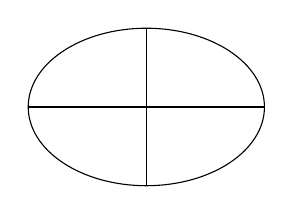
\begin{tikzpicture}
    \draw (0,0) ellipse (1.5 and 1);
    \draw (-1.5,0) -- (1.5,0);
    \draw (0,-1) -- (0,1);
\end{tikzpicture}
\end{center}

$\atoms(A_1, A_2) = \{A \in A_* : A \neq \varnothing\}$

$\field(A_1, A_2) = $ the set of all possible unions of elements of $\atoms (A_1, A_2)$.

Next, if $A_1,A_2,A_3,\dots \subseteq \Omega$, what is $\field (A_1,A_2,A_3,\dots)$?

\begin{lemma}
Let $\Phi$ be an upwards directed set of fields of sets of $\Omega$. Then let $\mathscr{G} = \bigcup \Phi$. Then $\mathscr{G}$ is a field of subsets of $\Omega$.
\end{lemma}
\begin{proof}
    To say $\Phi$ is upwards directed means for $\mathscr{F}_1, \mathscr{F}_2 \in \Phi$, there exists $\mathscr{F}_3 \in \Phi$ such that $\mathscr{F}_1, \mathscr{F}_2 \subseteq \mathscr{F}_3$.
    We have $\varnothing, \Omega \in \mathscr{G}$ because there is $\mathscr{F} 
    \in \Phi$ and $\varnothing, \Omega \in \mathscr{F}$.
    
    Let $A \in \mathscr{G}$. Then $A \in \mathscr{F}$ for some $\mathscr{F} \in \Phi$. Now, $\mathscr{F}$ is a field on $\Omega$, so $\Omega \setminus A \in \mathscr{F}$ and hence $\Omega \setminus A \in \mathscr{G}$.
    
    Now let $A_1, A_2 \in \mathscr{G}$. Then for some $\mathscr{F}_1, \mathscr{F}_2 \in \Phi$, we have $A_1 \in \mathscr{F}_1$, $A_2 \in \mathscr{F}_2$.
    
    Since $\Phi$ is upwards directed, there exists $\mathscr{F}_3 \in \Phi$ such that $\mathscr{F_1} \subseteq \mathscr{F}_3$ and $\mathscr{F}_2 \subseteq \mathscr{F}_3$. But $\mathscr{F}_3$ is a field on $\Omega$. Hence, $A_1 \cup A_2 \in \mathscr{F}_3$ and therefore $A_1 \cup A_2 \in \mathscr{G}$.
    
    Thus $\mathscr{G}$ is a field on $\Omega$.
\end{proof}

\begin{proposition}
    Let $(\F_n)_{n \in \N}$ be an increasing sequence of fields on $\Omega$. Let $\mathscr{G = \bigcup_n \mathscr{F}_n}$. Then $\mathscr{G}$ is a field on $(\F_n)_{n \in \N}$.
\end{proposition}

\begin{proof}
    Apply the lemma with $\Phi = \{\F_n : n \in \N\}$. (Let $n_1,n_2 \in \N$. Let $n_3 = \max\{n_1,n_2\}$. Then $\mathscr{F}_{n_1} \subseteq \mathscr{F}_{n_2}$ and $\mathscr{F}_{n_2} \subseteq \mathscr{F}_{n_3}$.)
\end{proof}

\begin{corollary}
    Let $(A_n)_{n \in \N}$ be a sequence of subsets of $\Omega$. Then
    \[\field (A_1,A_2,A_3\dots) = \bigcup_{n \in \N} \field(A_1,\dots,A_n).\]
\end{corollary}

\begin{proof}
    For each $n \in \N,\ \field(A_1,\dots,A_{n+1})$ contains $A_1,\dots,A_n$, so $$\field(A_1,\dots,A_n) \subseteq \field(A_1,\dots,A_n, A_{n+1}).$$

    Hence $\bigcup_{n \in \N} \field(A_1,\dots,A_n)$ is a field on $\Omega$ that contains $A_1,A_2,A_3,\dots$ and any field on $\Omega$ that contains $A_1,A_2,A_3,\dots$ must contain $\bigcup_{n \in \N} \field(A_1,\dots,A_n)$.
\end{proof}

\begin{definition}
    A field is \textit{complete} if it is closed under arbitrary unions and intersections.
\end{definition}

\begin{theorem}
    Let $\mathscr{G} \subseteq \mathcal{P}(\Omega)$. Define $X: \Omega \to \{0,1\}^{\mathscr{G}}$ by $X(\omega) = (1_G (\omega))_{G \in \mathscr{G}}$. Let $\mathscr{B} = \{B \subseteq \Omega : 1_B \eit \ X\}$. Let $\mathbf{X} = X[\Omega]$. Then
    \begin{enumerate}[(a)]
        \item $C \mapsto X^{-1}[C]$ is a bijection from $\mathcal{P}(\mathbf{X})$ onto $\mathscr{B}$.
        \item $|\mathscr{B}| = |\mathcal{P}(\mathbf{X})|$
        \item $\mathscr{B}$ is the smallest complete field on $\Omega$ containing $\mathscr{G}$
    \end{enumerate}
\end{theorem}

\begin{remark}
    \begin{enumerate}[(a)]
        \item This is just proved as in the case where $\mathscr{G}$ is finite.
        \item Since a finite field is a complete field, this theorem includes the earlier one as a special case.
    \end{enumerate}
\end{remark}

\begin{example}
Suppose $\Omega = \Z$ and $\mathscr{G} = \{ \{n\} : n \in \Z\}$. Then $\field (\mathscr{G}) = \{A \subseteq \Z : A$ is finite or $\Z\setminus A$ is finite $\}$.
\end{example}

The complete field on $\Z$ generated by $\mathscr{G}$ is $\mathcal{P}(\Z)$

\begin{definition}
    To say $\mathscr{H}$ is a $\pi$-system on $\Omega$ means $\mathscr{H}$ is a collection of subsets of $\Omega$ and for all $A,B \in \mathscr{H}$ we have $A \cap B \in \mathscr{H}$.
\end{definition}

\begin{proposition}
    Let $\mathscr{E} \subseteq \mathcal{P}(\Omega)$. Let $\mathscr{H} = \{ \cap \mathscr{E}_0 : \varnothing \neq \mathscr{E}_0 \ \text{finite} \ \subseteq \mathscr{E}\}$. Then $\pi(\mathscr{E}) = \mathscr{H}$ is the smallest $\pi$-system containing $\mathscr{E}$.
\end{proposition}



\begin{proof}
    First, let's show $\mathscr{H}$ is a $\pi$-system. Let $A_1, A_2 \in \mathscr{H}$. Then $A_1 = \cap \mathscr{E}_1$, $A_2 = \mathscr{E}_2$ for some nonempty finite $\mathscr{E}_1,\mathscr{E}_2 \subseteq \mathscr{E}$.
    Then $A_1 \cap A_2 = \cap \mathscr{E}_3$, where $\mathscr{E}_3 = \mathscr{E}_1 \cap \mathscr{E}_2$ (For each $\omega$ we have $\omega \in A_2 \cap A_2$ iff $\omega \in A_1$ and $\omega \in A_2$ iff $\omega \in E$ for each $E \in \mathscr{E}_1$ and $\omega \in E$ for each $E \in \mathscr{E}_2$ iff $\omega \in E$ for each $E \in \mathscr{E}_1 \cup \mathscr{E}_2$.)
    Now $\mathscr{E} \neq \varnothing$ since $\mathscr{E}_1 \neq \mathscr{E}_1$.
    Also, $\mathscr{E}_3$ is finite, since $\mathscr{E}_1,\mathscr{E}_2$ are both finite. Thus $A_1 \cap A_2 \in \mathscr{H}$, therefore $\mathscr{H}$ is a $\pi$-system.
    
    Suppose $\mathscr{H}'$ is a $\pi$-system that contains $\mathscr{E}$. We wish to show $\mathscr{H} \subset \mathscr{H}'$. Let $A \in \mathscr{H}$. By the definition of $\mathscr{H},\ A = \cap \mathscr{E}_0$ for some nonempty finite $\mathscr{E}_0 \subseteq \mathscr{E}$. Since $\mathscr{E} \subseteq \mathscr{H}'$ and $\mathscr{H}'$ is a $\pi$-system, $\cap \mathscr{E}_0 \in \mathscr{H}'$
\end{proof}

\section*{2/1/21}

\begin{proposition}
    Let $(\mathscr{E}_i)_{i \in I}$ be a family of $\pi$-systems. Then $$\pi\left(\bigcup_{i \in I} \mathscr{E}_i\right) = \left\{\bigcap_{i \in I_0} E_i : \varnothing \neq I_0 \text{ finite } \subseteq I \text{ and } E_i \in \mathscr{E}_i \text{ for } i \in I_0\right\}$$
\end{proposition}

\begin{proof}
    Clearly
    $$\pi\left(\bigcup_{i \in I} \mathscr{E}_i\right) \supseteq \left\{\bigcap_{i \in I_0} E_i : \varnothing \neq I_0 \text{ finite } \subseteq I \text{ and } E_i \in \mathscr{E}_i \text{ for } i \in I_0\right\}.$$
    Hence it suffices to show that the right hand side is in fact a $\pi$-system.
    Let $E, F$ be elements of the right hand side. Now, $E = \bigcap_{i \in I_1} E_i$ for some nonempty finite $I_1 \subseteq I$ and some $E_i \in \mathscr{E}_i, i \in I_1$.
    Likewise, $F = \bigcap_{i \in I_2} F_i$ for some nonempty finite $I_2 \subseteq I$ and some $F_i \in \mathscr{E}_i, i \in I_2$.
    Let $I_3 = I_1 \cup I_2$. For $i \in I_3$, let
    $$G_i = 
    \begin{cases}
        E_i &\text{if } i \in I_1 \setminus I_2, \\
        F_i &\text{if } i \in I_2 \setminus I_1 \\
        E_i \cap F_i &\text{if } i \in I_1 \cap I_2
    \end{cases}$$
    Then $G_i \in \mathscr{E}_i$ for each $i \in I_3$, since $\mathscr{E}_i$ is a $\pi$-system.
    Then $E \cap F = \bigcap_{i \in I_3} G_i$ is an element of the right hand side.
\end{proof}

\subsection*{Pokemon theory (gotta collect 'em all).}
If $\mathscr{A} = \{ A_i : i \in I\}$, where $I \neq \varnothing$, then $\bigcap \mathscr{A} = \bigcap_{i \in I} A_i$. Any $\mathscr{B}$ is of the form $\{B_j : j \in J\}$ for some $(B_j)_{j \in I'}$. Just let $J = \mathscr{B}$ and let $B_j = j$ for each $j \in J$.

\begin{definition}
Let $(\Omega, \F, P)$ be a probability space.
Let $(\mathscr{E}_i)_{i \in I}$ be a family of $\pi$-systems such that for each $i \in I$, $\mathscr{E}_i \subseteq \F$. To say that $(\mathscr{E}_i)_{i \in I}$ is \emph{independent} means that for each nonempty finite $I_0 \subseteq I$ and for all $E_i \in \mathscr{E}_i$, $i \in I_0$, we have $P(\bigcap_{i \in I_0} E_i) = \prod_{i \in I_0} P(E_i)$.
\end{definition}

\begin{example}
A family $(A_i)_{i \in I}$ is independent if and only if the family $(\{A_i\})_{i \in I}$ is independent. %(why? lol)
\end{example}

\begin{theorem}[The Grouping Theorem, Version 1.]
    Let $(\mathscr{G}_i)_{i \in I}$ be an independent family of $\pi$-systems. Let $(I_j)_{j \in J}$ be a disjoint family of nonempty subsets of $I$. Let
    $$\mathscr{H}_j = \pi \left(\bigcup_{i \in I_j} \mathscr{G}_i \right)$$
    Then the family of $\pi$-systems $(\mathscr{H}_j)_{j \in J}$ is independent.
\end{theorem}

\begin{proof}
    Let $\varnothing \neq J_0$ finite $\subseteq J$, and let $H_j \in \mathscr{H}_j$ for each $j \in J_0$.
    We wish to show that $P\p{\bigcap_{j \in J_0} H_j} = \prod_{j \in J_0} P(H_j)$.
    Since each $\mathscr{G}_i$ is a $\pi$-system and $\mathscr{H}_j = \pi\p{\bigcup_{i \in I_j} \mathscr{G}_i}$ for each $j \in J_0$, there exists a nonempty finite set $I_j^0 \subseteq I_j$ and sets $G_i \in \mathscr{G}_i, i \in I_j^0$ such that
    $H_j = \bigcap_{i \in I_j^0} G_i$.
    Then 
    \begin{align*}
        P\left( \bigcap_{j \in J_0} H_j \right) &= P\left( \bigcap_{j \in J_0} \bigcap_{i \in I_j^0} G_i \right) = P\left( \bigcap_{i \in I^0} G_i \right) \\
        \intertext{where $I^0 = \bigcup_{j \in J_0} I_j^0$. By independence of $(\mathscr{G}_i)_{i \in I}$, this is}
        &= \prod_{i \in I^0} P(G_i) = \prod_{j \in J_0} \prod_{i \in I^0_j} P(G_i) = \prod_{j \in J_0} P \left( \bigcap_{i \in I^0_j} G_i \right) = \prod_{j \in J_0} P(H_j)
    \end{align*}
    as desired.
\end{proof}

Let $X$ be a set. For each $A \subseteq X$, let $A^c = X \setminus A$

\begin{definition}
To say $\mathscr{B}$ is a \emph{$\lambda$-system} on $X$ means $\mathscr{B} \subseteq \mathcal{P}(X)$ such that
\begin{enumerate}[(a)]
    \item $X \in \mathscr{B}$
    \item For all $B \in \mathscr{B},\ B^c \in \mathscr{B}$
    \item For each disjoint $(B_n) \in \mathscr{B}^{\N}$,\ $\bigcupdot_{n \in \N} B_n \in \mathscr{B}$
\end{enumerate}
\end{definition}

\begin{example}
    Let $\mu$ and $\nu$ be measures on $\sigma$-field $\mathscr{A}$ on $X$ and let $\mathscr{B} = \{B \in \mathscr{A} : \mu(B) = \nu(B) \}$. Then $\mathscr{B}$ need not be closed under countable unions, but it is closed under countable disjoint unions.
    If in addition $\mu(X) = \nu(X) < \infty$, then $\mathscr{B}$ is a $\lambda$ system on $X$.
\end{example}

\begin{definition}[belated]
    Let $\mathscr{A}$ be a $\sigma$-field on $X$. To say $\mu$ is a \emph{measure} on $\mathscr{A}$ means $\mu: \mathscr{A} \to [0,\infty]$, such that;
    \begin{enumerate}[(a)]
        \item $\mu(\varnothing) = 0$
        \item For each disjoint sequence $(A_n) \in \mathscr{A}^{\N}$,\ $\mu\left( \bigcup_{n \in \N} A_n \right) = \sum_{n \in \N} \mu(A_n)$
    \end{enumerate}
\end{definition}

\subsection*{Some properties of measures.}

Let $\mu$ be a measure on a $\sigma$-field $\mathscr{A}$ on $X$.

\begin{enumerate}[(a)]
    \item For each $n \in \N$, for all disjoint $A_1,\dots,A_n \in \mathscr{A},\  \mu \left( \bigcup_{k=1}^n A_k \right) = \sum_{k=1}^n \mu(A_k)$
    \begin{proof}
        Let $A_k = \varnothing$ for $k > n$.
    \end{proof}
    \item For all $A, B \in \mathscr{A}$, if $A \subseteq B$, then $\mu(A) + \mu(B \setminus A)= \mu(B)$, so $\mu(A) \leq \mu(B)$.
    If in addition $\mu(A) < \infty$, then $\mu(B \setminus A) = \mu(B) - \mu(A)$.
    \begin{proof}
        $A \sqcup (B \setminus A) = B$.
    \end{proof}
    \item For all $A, A_1, A_2, \dots \in \mathscr{A}$, if $A \subseteq \bigcup_n A_n$, then $\mu(A) \leq \sum_n \mu(A_n)$
    \begin{proof}
        By (b), it suffices to consider the case where $A = \bigcup_n A_n$. Let $E_n = A_n \setminus \bigcup_{m < n} A_m$. Then $E_1, E_2, \dots$ are disjoint with $A = \bigcupdot_n E_n$.
        Hence $\mu(A) = \sum_n \mu(E_n) \leq \sum_n \mu(A_n)$, again by (b) since $E_n \subseteq A_n$.
    \end{proof}
    \item For each increasing sequence $(A_n) \in \mathscr{A}^{\N}$, if $A = \bigcup_u A_n$ then $\mu(A_n) \xrightarrow[n \to \infty]{\text{increases}} \mu(A)$.
    \begin{proof}
        Let $B_1 = A_1$, for $n \geq 2$ let $B_n = A_n \setminus A_{n-1}$. Then $B_1, B_2, \dots$ are disjoint, $\bigcup_{k \in \N} B_k = A$, and for each $n$ $\bigcup_{k=1}^n B_k = A_n$.
        Hence $\mu(A_n) = \sum_{k=1}^n \mu(B_k)$ increases to $\sum_{k \in \N} \mu(B_k) = \mu(A)$.
    \end{proof}
    \item For each decreasing sequence $(A_n) \in \mathscr{A}^{\N}$, if $\mu(A_1) < \infty$, then $\mu(A_n) \xrightarrow[n \to \infty]{\text{decreases}} \mu(A)$ where $A = \bigcap_n A_n$.
    \begin{proof}
        Let $B_n = A_1 \setminus A_n$. Then $B_1 \subseteq B_2 \subseteq \cdots$ with $B = \bigcup_n B_n A_1 \setminus \bigcap_n A_n$. By (d), $\mu(B_n)$ increases to $\mu(B)$.
        Hence $\mu(A_1) - \mu(B_n) = \mu(A_1 \setminus B_n) = \mu(A_n)$ decreases to $\mu(A_1) - \mu(B) = \mu(A_1 \setminus B) = \mu(A)$.
    \end{proof}
    \begin{remark}
        We need the assumption that $\mu(A_1) < \infty$.
        For example, define $\mu$ on $\mathcal{P}(\N)$ by
        \[
            \mu(A) = \begin{cases}
                |A| &\text{if } A \text{ is finite} \\ \infty &\text{if } A \text{ is infinite}
            \end{cases}
        \]
        and let $A_n = \{n, n+1, \dots\}$. Then $\mu(A_n) = \infty$ for each $n$ with $A_1 \supseteq A_2 \supseteq \cdots$ and $\bigcap_n A_n = \varnothing$. Hence $\mu(A_n) \neq \mu(\bigcap_n A_n)$.
    \end{remark}
\end{enumerate}

\section*{2/3/21}
\subsection*{Finite(-ish) $\lambda$-systems.}
Let $X$ be a set.
\begin{definition}
    To say $\mathscr{B}$ is a \bm{$\lambda_0$}\emph{-system on} \bm{$X$} means that $\mathscr{B} \subseteq \mathcal{P}(X)$ and
    \begin{enumerate}[(a)]
        \item $X \subseteq \mathscr{B}$
        \item For each $B \in \mathscr{B}$, $B^c \in \mathscr{B}$
        \item For all disjoint $A, B \in \mathscr{B}$, $A \sqcup B \in \mathscr{B}$
    \end{enumerate}
\end{definition}

\begin{proposition}
    Let $\mathscr{B} \subseteq \mathcal{P}(X)$. The following are equivalent:
    \begin{enumerate}[(a)]
        \item $\mathscr{B}$ is a $\lambda_0$-system on $X$
        \item $X \in \mathscr{B}$ and for all $A, B \in \mathscr{B}$, if $A \subseteq B$ then $B \setminus A \in \mathscr{B}$.
    \end{enumerate}
\end{proposition}
\begin{proof}
    (a) $\implies$ (b). Supposeing (a), we have $X \in \mathscr{B}$. Let $A, b \in \mathscr{B}$ and suppose $A \subseteq B$. Then $A$ and $B^c$ are disjoint elements of $\mathscr{B}$, so $A \cup B^c \in \mathscr{B}$, so $(A \cup B^c)^c \in \mathscr{B}$.
    But $(A \cup B^c)^c = A^c \cap B^{cc} = A^c \cap B = B \setminus A$. Thus $B \setminus A \in \mathscr{B}$ and hence (a) implies (b).
    
    (b) $\implies$ (a). We have $X \in \mathscr{B}$ by assumption. Let $B \in \mathscr{B}$. Then $B, X \in \mathscr{B}$ and $B \subseteq X$, so $B^c = X \setminus B \in \mathscr{B}$.
    Let $A, B \in \mathscr{B}$ with $A \cap B = \varnothing$. We want to show that $A \cup B \in \mathscr{B}$. Since  $A \cap B = \varnothing$, $A \subseteq B^c = X \setminus B$, and of course $B^c \in \mathscr{B}$, so $B^c \setminus A \in \mathscr{B}$, so $(B^c \setminus A)^c = (B^c \cap A^c)^c = B^{cc} \cup A^{cc} = A \cup B \in \mathscr{B}$, as desired. This shows that (b) implies (a).
\end{proof}

\begin{proposition}
    Let $\mathscr{B}$ be a $\lambda_0$-system on $X$ and let $A, B \in \mathscr{B}$. Then the following are equivalent:
    \begin{enumerate}[(a)]
        \item $A \cap B \in \mathscr{B}$
        \item $A \setminus B \in \mathscr{B}$
        \item $A \cup B \in \mathscr{B}$
        \item $B \setminus A \in \mathscr{B}$
    \end{enumerate}
\end{proposition}
\begin{proof}
    Suppose $A \cap B \in \mathscr{B}$. Now $A \cap B \subseteq A$, which by the previous proposition means $A \setminus (A \cap B) \in \mathscr{B}$. But $A \setminus (A \cap B) = A \setminus B$, hence $A \setminus B \in \mathscr{B}$ so (a) implies (b).
    
    Now suppose that $A \setminus B \in \mathscr{B}$. Then $A \setminus B$ and $B$ are disjoint elements of $\mathscr{B}$, so $(A \setminus B) \cup B = A \cup B \in \mathscr{B}$. Hence (b) implies (c).
    
    Now suppose $A \cup B \in \mathscr{B}$. Now $A \subseteq A \cup B$ so $(A \cup B) \setminus A = B \setminus A \in \mathscr{B}$ and thus (c) implies (d).
    
    Finally, suppose $B \setminus A \in \mathscr{B}$. Now $B \setminus A \subset B$, so $B \setminus (B \setminus A) = A \cap B \in \mathscr{B}$, so (d) implies (a).
\end{proof}

\begin{lemma}
Let $\mathscr{B}$ be a $\lambda_0$-system on $X$. Let $A_1, \ldots, A_n \subseteq X$ such that $\pi(A_1, \ldots, A_n) \subseteq \mathscr{B}$. Let $k \in \{1, \ldots, n\}$ and let $B_k = A_k^c$. For $j \neq k$, let $B_j = A_j$. Then $\pi(B_1, \ldots, B_n) \subseteq \mathscr{B}$.
\end{lemma}
\begin{proof}
    Let $C \in \pi(B_1, \ldots, B_n)$. Then $C = \bigcap_{j \in J} B_j$ for some nonempty $J \subseteq \{1, \ldots, n\}$. We wish to show that $C \in \mathscr{B}$.
    If $k \notin J$, then clearly this holds because then $C = \bigcap_{j \in J} A_j \in \pi(A_1, \ldots, A_n) \subseteq \mathscr{B}$. Suppose $k \in J$. If $J = \{k\}$ then $C = A_k^c \in \mathscr{B}$.
    Suppose $J \neq \{k\}$. Then let $J' = J \setminus\{k\}$. Then $\varnothing \neq J' \subseteq \{1, \ldots, n\}$.
    Let $D = \bigcap_{j \in J'} A_j$. Then $D \in \pi(A_1, \ldots, A_n) \subseteq \mathscr{B}$.
    Now, $D \cap A_k \in = \bigcap_{j \in J} A_j \in \pi(A_1, \ldots, A_n) \subseteq \mathscr{B}$. Hence by the previous proposition, $B \setminus A_k \in \mathscr{B}$.
    But $D \setminus A_k^ = D \cap A_k^c = D \cap B_k = \bigcap_{j \in J} B_j = C$, so $C \in \mathscr{B}$.
    This holds for each such $C \in \pi(B_1, \ldots, B_n)$, hence $\pi(B_1, \ldots, B_n) \subseteq \mathscr{B}$.
\end{proof}

\begin{proposition}
    Let $A_1, \ldots, A_n \subseteq X$. Suppose $\pi(A_1, \ldots, A_n) \subseteq \mathscr{B}$. For $k = 1, \ldots, n$, let $B_k\in \{A_k, A_k^c\}$. Then $\pi(B_1, \ldots, B_n) \subseteq \mathscr{B}$.
\end{proposition}
\begin{proof}
    Let $m$ be the number of $j \in \{1, \ldots, n\}$ such that $B_j = A_j^c$. Then the stated result follows by $m$ applications of the lemma.
\end{proof}

\begin{proposition}
    Let $A_1, \ldots, A_n \subseteq X$. Let $\mathscr{B}$ be a $\lambda_0$-system on $X$ such that $\pi(A_1, \ldots, A_n) \subseteq \mathscr{B}$. Then:
    \begin{enumerate}[(a)]
        \item $\atoms(A_1, \ldots, A_n) \subseteq \mathscr{B}$
        \item $\field(A_1, \ldots, A_n) \subseteq \mathscr{B}$
    \end{enumerate}
\end{proposition}
\begin{proof}
    Let $A \in \atoms(A_1, \ldots, A_n)$. Then there exist $B_j \in \{A_j, A_j^c\}$ for $j = 1, \ldots, n$ such that $\varnothing \neq A = \bigcap_{j=1}^n B_j$. Then $A \in \pi(B_1, \ldots, B_n) \subseteq \mathscr{B}$ by the previous proposition, establishing (a).
    
    We know that $\atoms(A_1, \ldots, A_n)$ is a finite (at most cardinality $2^n$) partition of $X$ and $\field(A_1, \ldots, A_n)$ is the set of all possible (disjoint) unions of the atoms, completing the proof.
\end{proof}

\begin{theorem}[$\pi$-$\lambda_0$ Theorem]
    Let $\mathscr{H}$ be a $\pi$-system on $X$ and let $\mathscr{B}$ be a $\lambda_0$-system on $X$ such that $\mathscr{H} \subseteq \mathscr{B}$. Then $\field(\mathscr{H}) \subseteq \mathscr{B}$.
\end{theorem}
\begin{proof}
    Let $\Phi$ be the set of finite subsets of $\mathscr{H}$. By the previous proposition, for each $\mathscr{H}_0 \in \Phi$, $\field(\mathscr{H}_0) \subseteq \mathscr{B}$.
    ($\pi(\mathscr{H}_0) \subseteq \pi(\mathscr{H} \subseteq \mathscr{B}$ so $\field(\pi(\mathscr{H}_0)) \subseteq \mathscr{B}$.)
    But $\field(\pi(\mathscr{H}_0)) = \field(\mathscr{H}_0)$. This holds for each $\mathscr{H}_0 \in \Phi$.
    
    But recall that $\field(\mathscr{H}) = \bigcup \{\field(\mathscr{H}_0) : \mathscr{H}_0\text{ finite } \subseteq \mathscr{H \}}$, so $\field(\mathscr{H}) \subseteq \mathscr{B}$.
\end{proof}

Let $(\Omega, \F, P)$ be a probability space.
\begin{lemma}
Let $(\mathscr{H}_i)_{i \in I}$ be an independent family of $\pi$-systems. For each $i \in I$, let $\F_i = \field(\mathscr{H}_i)$. Then $(\F_i)_{i \in I}$ is independent.
\end{lemma}
\begin{proof}
    Let $I_0$ be a nonempty finite subset of $I$ and let $F_i \in \F_i$ for $i \in I_0$.
    Let $F = \bigcap_{i \in I_0} F_i$. we want to show $P(F) = \prod_{i\in I_0} P(F_i)$.
    If $I_0 = 1$, then we are done.
    
    ???
\end{proof}

\section*{2/5/21}
\begin{definition}
    To say $\mathscr{M} \subseteq \mathcal{P}(X)$ is a \emph{monotone class} on $X$ means that each $(E_n) \in \mathscr{M}^{\N}$,
    \begin{enumerate}[(a)]
        \item If $E_n \subseteq E_{n+1}$ for each $n$, then $\bigcup_n E_n \in \mathscr{M}$.
        \item If $E_n \supseteq E_{n+1}$ for each $n$, then $\bigcap_n E_n \in \mathscr{M}$.
    \end{enumerate}
\end{definition}

\begin{proposition}
    Let $\mathscr{E} \subseteq \mathcal{P}(X)$. Then there is a smallest monotone class on $X$ containing $\mathscr{E}$.
    \begin{proof}
        Let $\mathscr{M}$ be the set of all $A \subseteq X$ such that $A \in \mathscr{N}$ for each monotone class $\mathscr{N}$ on $X$ such that $\mathscr{E} \subseteq \mathscr{N}$.
        Then for each monotone class $\mathscr{N}$ on $X$ such that $\mathscr{E} \subseteq \mathscr{N}$, we have $\mathscr{E} \subseteq \mathscr{M} \subseteq \mathscr{N}$, by definition of $\mathscr{M}$.
        It remains to show that $\mathscr{M}$ is a monotone class. Let $(E_n) \in \mathscr{M}^{\N}$;
        
        \begin{enumerate}[(a)]
            \item  Suppose $E_n \subseteq E_{n+1}$ for each $n$. Let $E = \bigcup_n E_n$. We wish to show that $E \in \mathscr{M}$. Let $\mathscr{N}$ be a monotone class on $X$ such that $\mathscr{E} \subseteq \mathscr{N}$. Each $E_n \in \mathscr{N}$. Hence $\bigcup_n E_n \in \mathscr{N}$ since $\mathscr{N}$ is a monotone class; in other words $E \in \mathscr{N}$. As this holds for arbitrary such $\mathscr{N}$, then $E \in \mathscr{M}$.
            \item Now suppose $E_n \supseteq E_{n+1}$ for each $n$. Then by a similar argument to (a) we have $\bigcap_n E_n \in \mathscr{M}$.
        \end{enumerate}
        Thus $\mathscr{M}$ is a monotone class.
    \end{proof}
\end{proposition}

\begin{proposition}
    Let $\mathscr{B}$ be a $\lambda$-system on $X$. Then $\mathscr{B}$ is a monotone class on $X$.
\end{proposition}
\begin{proof}
    Let $(E_n) \in \mathscr{B}^{\N}$ such that $E_n \subseteq E_{n+1}$ for all $n$. We want to show $\bigcup_n E_n \in \mathscr{B}$. Let $B_1 = E_1,\ B_2 = E_2 \setminus E_1,\ B_3 = E_3 \setminus E_2$, and so on. Then $B_1,\ B_2,\ B_3,\dots$ are disjoint and $\bigcup_n B_n = E$. Note that each $B_n \in \mathscr{B}$ because $E_{n-1} \subseteq E_n$ for each $n \geq 2$. Thus $E$ is a countable disjoint union of elements of $\mathscr{B}$ and hence an element of $\mathscr{B}$.
    
    Now let $(F_n) \in \mathscr{B}^{\N}$ such that $F_n \supseteq F_{n+1}$ for all $n$. Let $E_n = F_n^c$. Then $E_n \in \mathscr{B}$ and $E_n \subseteq E_{n+1}$, so by the previous argument $\bigcup_n E_n \in \mathscr{B}$. Hence $\bigcap_n F_n = \bigcap_n E_n^c = \left( \bigcup_{n} E_n \right)^c \in \mathscr{B}$.
\end{proof}

\begin{remark}
    We see that every $\lambda$-system is a monotone class, and every $\lambda_0$-system is a $\lambda$-system iff it is a monotone class.
\end{remark}

\begin{lemma}
    Let $\mathscr{F} \subseteq \mathcal{P}(X)$. Let $\mathscr{M}$ be the monotone class generated by $\mathscr{F}$. Then;
    
    \begin{enumerate}[(a)]
        \item $\bigcup_n E_n \in \mathscr{M}$ for each $(E_n) \in \mathscr{M}^{\N}$ iff $A \cup B \in \mathscr{M}$ for all $A,B \in \mathscr{F}$.
        \item $\bigcap_n E_n \in \mathscr{M}$ for each $(E_n) \in \mathscr{M}^{\N}$ iff $A \cap B \in \mathscr{M}$ for all $A,B \in \mathscr{F}$.
        \item $X\setminus E \in \mathscr{M}$ for each $E \in \mathscr{M}$ iff $X\setminus A \in \mathscr{M}$ for each $A \in \mathscr{F}$.
    \end{enumerate}
\end{lemma}
\begin{proof}
    \begin{enumerate}[(a)]
        \item ($\implies$) is obvious since $\F \subseteq \mathscr{M}$; take $E_1 = A, A_n = B$ for $n \geq 2$.
        
        ($\impliedby$) Suppose $A \cup B \in \mathscr{M}$ for all $A, B \in \F$. Let $A \in \F$, let $\mathscr{B} = \{B \subseteq X : A \cup B \in \mathscr{M}\}$. Then $\F \subseteq \mathscr{B}$.
        Let $(B_n) \in \mathscr{B}^{\N}$.
        \begin{enumerate}[(i)]
            \item Suppose $B_n \subseteq B_{n+1}$ for all $n$. Then $A \cup B_n \in \mathscr{M}$ and $A \cup B_n \subseteq A \cup B_{n+1}$ for all $n$.
            Hence $\bigcup_n (A \cup B_n) \in \mathscr{M}$. But $\bigcup_n (A \cup B_n) = A \cup \left(\bigcup_n B_n\right) \in \mathscr{B}$ by the definition of $\mathscr{B}$.
            \item Now suppose $B_n \supseteq B_{n+1}$ for all $n$. Then $A \cup B_n \in \mathscr{M}$ and $A \cup B_n \supseteq A \cup B_{n+1}$ for all $n$.
            Hence $\bigcap_n (A \cup B_n) \in \mathscr{M}$ since $\mathscr{M}$ is a monotone class. But $\bigcup_n (A \cup B_n) = A \cup \left(\bigcap_n B_n \right) \in \mathscr{M}$. Thus $\bigcap_n B_n \in \mathscr{B}$ by the definition of $\mathscr{B}$.
        \end{enumerate}
        We conclude that $\mathscr{B}$ is a monotone class containing $\F$. But $\mathscr{M}$ is the smallest such monotone class, so $\mathscr{M} \subseteq \mathscr{B}$ so for each $B \in \mathscr{M}$, $A \cup B \in \mathscr{M}$.
        This holds for each $A \in \F$.
        
        Let $B \in \mathscr{M}$. Let $\mathscr{A} = \{A \subseteq X : A \cup B \in \mathscr{M}\}$. Then $\F \subseteq \mathscr{A}$. Also, $\mathscr{A}$ is a monotone class by a similar argument, so $\mathscr{M} \subseteq \mathscr{A}$ and hence for all $A, B \in \mathscr{M}$, $A \cup B \in \mathscr{M}$.
        
        Let $(E_n) \in \mathscr{M}^{\N}$. Let $A_1 = E_1$, $A_2 = E_1 \cup E_2$, $A_3 = E_1 \cup E_2 \cup E_3$ and so on. Then each $A_n \in \mathscr{M}$ and $A_n \subseteq A_{n+1}$ for all $n$. Hence $\bigcup_n E_n = \bigcup_n A_n \in \mathscr{M}$, since $\mathscr{M}$ is a monotone class.
        \item Similar to (a).
        \item Simpler than (a).
    \end{enumerate}
\end{proof}

\begin{theorem}[Monotone Class Theorem]
    Let $\mathscr{F}$ be a field on $X$ and let $\mathscr{M}$ be a monotone class on $X$ generated by $\mathscr{F}$. Then $\mathscr{M}$ is a $\sigma$-field on $X$. Indeed, $\mathscr{M}$ is the smallest $\sigma$-field on $X$ containing $\mathscr{F}$.
\end{theorem}

\begin{proof}
    That $\mathscr{M}$ is a $\sigma$-field on $X$ follows immediately from the lemma.
    Let $\mathscr{N}$ be a $\sigma$-field on $X$ with $\F \subseteq \mathscr{N}$. Then $\mathscr{N}$ is a monotone class on $X$, so $\mathscr{M} \subseteq \mathscr{N}$.
\end{proof}

\begin{remark}
    For any $\pi$-system $\mathscr{H}$ on $X$, there exists a $\sigma$-field generated by $\mathscr{H}$, which is the smallest $\sigma$-field containing $\mathscr{H}$.
\end{remark}

\begin{theorem}[The $\pi$-$\lambda$ Theorem]
    Let $\mathscr{H}$ be a $\pi$-system on a set $X$, let $\mathscr{A}$ be the $\sigma$-field on $X$ generated by $\mathscr{H}$, and let $\mathscr{B}$ be a $\lambda$-system on $X$ containing $\mathscr{H}$. Then $\mathscr{A} \subseteq \mathscr{B}$
    \begin{proof}
        Let $\mathscr{M}$ be the monotone class on $X$ generated by $\field(\mathscr{H})$. By the monotone class theorem $\mathscr{M}$ is a $\sigma$-field on $X$. Thus $\mathscr{A} \subseteq \mathscr{M}$. (In fact, $\mathscr{A} = \mathscr{M}$.)
        
        The $\pi$-system $\mathscr{H}$ is contained in the $\lambda_0$-system $\mathscr{B}$ (since any $\lambda$-system is a $\lambda_0$-system) so by the $\pi-\lambda_0$ theorem, $\field(\mathscr{H}) \subseteq \mathscr{B}$. But $\mathscr{B}$ is a monotone class, since it is a $\lambda$-system, so $\mathscr{M} \subseteq \mathscr{B}$. Thus $\mathscr{A} \subseteq \mathscr{M} \subseteq \mathscr{B}$.
    \end{proof}
\end{theorem}

\section*{2/8/21}

\begin{theorem}
    Let $(X, \mathscr{A})$ be a measurable space and let $\mathscr{H}$ be a $\pi$-system on $X$ which generates the $\sigma$-field $\mathscr{A}$.
    Let $\mu$ and $\nu$ be finite measures on $\mathscr{A}$ such that $\mu(X) = \nu(X)$ and for each $H \in \mathscr{H}$, $\mu(H) = \nu(H)$.
    That $\mu = \nu$.
\end{theorem}

\begin{proof}
    Let $\mathscr{B} = \{B \in \mathscr{A} : \mu(B) = \nu(B)\}$. Since $\mu,\nu$ are measures on $\mathscr{A}$ and $\mu(X) = \nu(X),\ \mathscr{B}$ is a $\lambda$-system on $X$. Now let $\mathscr{H} \subseteq \mathscr{B}$, because $\mu(H) = \nu(H)$ for all $H \in \mathscr{H}$. Since $\mathscr{H}$ is a $\pi$-system on $X$, and $\mathscr{B}$ is a $\lambda$-system containing $\mathscr{A} = \sigma(\mathscr{H})$ (notationally, this means the $\sigma$-field generated by $\mathscr{H}$), we have $\sigma(\mathscr{H}) = \mathscr{A} \subseteq \mathscr{B}$ by the $\pi-\lambda$ theorem and thus $\mathscr{A} = \mathscr{B}$. Hence, $\mu = \nu$.
\end{proof}

\begin{corollary}
    Let $(X,\mathscr{A})$ be a measurable space. Let $\mathscr{H}$ be a $\pi$-system on $X$ such that $\sigma(\mathscr{H}) = \mathscr{A}$. Suppose $(H_n) \in \mathscr{H}^{\N}$ is a sequence of elements such that $\bigcup_n H_n = X$. Let $\mu,\nu$ be measures on $\mathscr{A}$ such that $\mu(H) = \nu(H)\ \forall H \in \mathscr{H}$ and assume that $\mu(H_n) = \nu(H_n) < \infty$ for all $n$. Then $\mu = \nu$.
\end{corollary}

\begin{proof}
    For each $n$, define $\mu_n,\ \nu_n$ on $\mathscr{A}$ by $\mu_n (A) = \mu(A \cap H_n)$ and $\nu_n (A) = \nu(A \cap H_n)$ and notice that $\mu_n$ and $\nu_n$ are finite measures on $\mathscr{A}$ satisfying $\mu_n (X) = \nu_n (X) < \infty$ and $\mu_n (H) := \mu (\underbrace{(H \cap H_n)}_{\in \mathscr{H}}) = \nu(\underbrace{(H \cap H_n)}_{\in \mathscr{H}}) = \nu_n (H)$, thus $\mu_n = \nu_n$ by the previous theorem.
    
    Let $A_n = A \cap H_n$. Then $A = A \cap X = A \cap (\bigcup_n H_n) = \bigcup_n (A \cap H_n) = \bigcup_n(A_n)$.
    Let $B_n = A_n \setminus \bigcup_{m < n} A_n$. Then $(B_n)$ is a disjoint sequence in $\mathscr{A}$ and $A = \bigcupdot_n B_n$.
    Now $\mu(B_n) = \mu_n(B_n) = \nu_n(B_n) = \nu(B_n)$.
    
    Hence $\mu(A) = \sum_n \mu(B_n) = \sum_n \nu(B_n) = \nu(A)$. This holds for each $A \in \mathscr{A}$. Hence $\mu = \nu$.
\end{proof}

\begin{remark}
    If $a = (a_1, \ldots, a_d) \in \R^d$ and $b = (b_1, \ldots, b_d) \in \R^d$, then $a \leq b$ means $a_k \leq b_k$ for each $k = 1, \ldots, d$ and $a < b$ means that $a_k < b_k$ for $k = 1, \ldots, d$.
    
    Also $(a, b] = \{x \in \R^d : a < x \leq b\} = \prod_{k=1}^d (a_k, b_k]$.
\end{remark}

\begin{corollary}
    Let $\mu, \nu$ be Borel measures on $\R^d$. Suppose $\mu((a,b]) = \nu((a,b]) < \infty$ for all $a, b \in \R^d$ with $a \leq b$. Then $\mu = \nu$.
\end{corollary}
\begin{proof}
    To say $\mu, \nu$ are Borel measures on $\R^d$ means they are measures on $\mathscr{A} = \sigma(\mathscr{G})$, where $\mathscr{G}$ is the set of open subsets of $\R^d$.
    Let $\mathscr{H} = \{ (a,b] : a, b \in \R^d, a \leq b \}$. Then $\mathscr{H}$ is a $\pi$-system.
    
    $\sigma(\mathscr{H}) = \sigma(\mathscr{G})$. Also, for each $n \in \N$, $(-n,n]^d \in \mathscr{H}$ and $\bigcup_n (-n, n]^d = \R^d$. Hence $\mu = \nu$ be the previous corollary.
\end{proof}

\begin{proposition}
    Let $\mathscr{H} \subseteq \mathcal{P}(X)$. Then there is a smallest $\sigma$-field $\mathscr{A}$ on $X$ containing $\mathscr{H}$.
\end{proposition}
\begin{proof}
    Let $\mathscr{A} = \{A \subseteq X : A \in \mathscr{B}$ for each $\sigma$-field $\mathscr{B}$ on $X$ with $\mathscr{H} \subseteq \mathscr{B} \}$. Then $\mathscr{A}$ is a $\sigma$-field on $X$, $\mathscr{H} \subseteq \mathscr{A}$, and for each $\sigma$-field $\mathscr{B}$ on $X$ such that $\mathscr{H} \subseteq \mathscr{B}$, we have $\mathscr{A} \subseteq \mathscr{B}$.
\end{proof}

\begin{remark}
    Let $\mathscr{H} \subseteq \mathcal{P}(X)$. Then $\sigma(\mathscr{H})$ denotes the smallest $\sigma$-field $\mathscr{A}$ on $X$ such that $\mathscr{H} \subseteq \mathscr{A}$.
    
    \emph{Warning:} $\sigma(\mathscr{H})$ depends on $X$ as well as on $\mathscr{H}$.
\end{remark}

\begin{proposition}
    Let $\mathscr{G}, \mathscr{H} \subseteq \mathcal{P}(X)$. Then $\sigma(\mathscr{G}) \subseteq \sigma(\mathscr{H})$ if and only if $\mathscr{G} \subseteq \sigma(\mathscr{H})$.
\end{proposition}
\begin{proof}
    ($\implies$) $\mathscr{G} \subseteq \sigma(\mathscr{G})$.
    
    ($\impliedby$) Suppose $\mathscr{G} \subseteq \sigma(\mathscr{H})$. Then $\sigma(\mathscr{H})$ is a $\sigma$-field on $X$ such that $\mathscr{G} \subseteq \sigma(\mathscr{H})$.
    But $\sigma(\mathscr{G})$ is the smallest such $\sigma$-field. Hence $\sigma(\mathscr{G}) \subseteq \sigma(\mathscr{H})$.
\end{proof}

\begin{corollary}
    Let $\mathscr{G}, \mathscr{H} \subseteq \mathcal{P}(X)$. Then $\sigma(\mathscr{G}) = \sigma(\mathscr{H})$ if and only if $\mathscr{G} \subseteq \sigma(\mathscr{H})$ and $\mathscr{H} \subseteq \sigma(\mathscr{G})$.
\end{corollary}

\begin{example}
    Let $\mathscr{A}$ be the Borel $\sigma$-field on $\R^d$ and let $\mathscr{H} = \{(a, b] : a, b \in \R^d, a \leq b\}$. Then $\mathscr{A} = \sigma(\mathscr{H})$.
    \begin{proof}
        By definition, $\mathscr{A} = \sigma(\mathscr{G})$, where $\mathscr{G}$ is the set of open subsets on $\R^d$. By the preceding corollary, to show that $\sigma(\mathscr{G}) = \sigma(\mathscr{H})$, it suffices to show that $\mathscr{G} \subseteq \sigma(\mathscr{H})$ and $\mathscr{H}\subseteq \sigma(\mathscr{G})$.
        
        Let $G \in \mathscr{G}$. Let $\mathscr{H}_0 = \{(a, b] : a, b \in \Q^d, a \leq b\}$.
        Then $\mathscr{H}_0$ is countable. Let $\mathscr{H}_1 = \{H \in \mathscr{H}_0 : H \subseteq \mathscr{G}\}$. Then $\mathscr{H}_1$ is a countable subset of $\mathscr{H}$ and $\bigcup \mathscr{H}_1 = G$. Then $G \in \sigma(\mathscr{H})$.
        This holds for each $G \in \mathscr{G}$, hence $\mathscr{G} \subseteq \sigma(\mathscr{H})$, so $\sigma(\mathscr{G}) \subseteq \sigma(\mathscr{H})$.
        
        Now let $H \in \mathscr{H}$. Then $H = (a, b]$ for some $a, b \in \R^d$ with $a \leq b$. We have $a = (a_1, \ldots, a_d)$, $b = (b_1, \ldots, b_d)$ for some $a_1, \ldots, a_d, b_1, \ldots b_d \in \R$ with $a_k \leq b_k$, $k = 1, \ldots, d$.
        For each $n \in \N$, let $G_n = \prod_{k=1}^d (a_k, b_k + \frac{1}{n})$. Then $G_n \in \mathscr{G}$ and $\bigcap_{n \in \N} G_n = H$. Hence $H \in \sigma(\mathscr{G})$. This holds for each $H \in \mathscr{H}$, hence $\mathscr{H} \subseteq \sigma(\mathscr{H})$, so $\sigma(\mathscr{H}) \subseteq \sigma(\mathscr{G})$.
    \end{proof}
\end{example}

\subsection*{Random variables.}
Let $(\Omega, \F, P)$ be a probability space.

\begin{example}
    Roll 2 dice. Let $X_1$ be the number from the first die and $X_2$ the number from the second. $X_1$ and $X_2$ are random variables. So is $X_1 + X_2$. The expected value of $X_1$, is
    \[
        E(X_1) = \sum_{k=1}^6 kP(X_1 = k) = \frac{1}{6}\sum_{k=1}^6 k = \frac{1}{6} \frac{6 \cdot 7}{2} = \frac{7}{2}.
    \]
    
    Similarly, $E(X_2) = 3.5$, and for $X_1 + X_2$ we have
    \[\begin{array}{c|c}
        k & P(X_1 + X_2 = k) \\ \hline
        2 & \sfrac{1}{36} \\
        3 & \sfrac{2}{36} \\
        4 & \sfrac{3}{36} \\
        5 & \sfrac{4}{36} \\
        6 & \sfrac{5}{36} \\
        7 & \sfrac{6}{36} \\
        8 & \sfrac{5}{36} \\
        9 & \sfrac{4}{36} \\
        10 & \sfrac{3}{36} \\
        11 & \sfrac{2}{36} \\
        12 & \sfrac{1}{36} \\
    \end{array}\]
    $E(X_1 + X_2) = \sum_{k=2}^{12} kP(X_1 + X_2 = k) = $ a mess $= 7$, or by linearity
    $E(X_1 + E_2) = E(X_1) + E(X_2) = 7$.
\end{example}

\begin{example}
    Roll a die repeatedly. Let $X$ be the number of rolls until a 5 is rolled.
    \begin{align*}
        P(X = 1) &= \frac{1}{6} = p \tag{$q = 1- p$} \\
        P(X = 2) &= qp \\
        P(X = 3) &= q^2 p \\
        &\vdots \\
        P(X = n) &= q^{n-1} p \tag{for $n \in \N$} \\
        P(X < \infty) &= \sum_{n \in \N} P(X = n) = \sum_{n=1}^\infty q^{n-1} p = p\sum_{k=0}^\infty q^k = p \frac{1}{1-q} = p\frac{1}{p} = 1.
    \end{align*}
    \begin{align*}
        E(X) &= \sum_{n=1}^\infty nP(X=n) = \sum_{n=1}^\infty npq^{n-1} \\
        qE(X) &= \sum_{n=1}^\infty npq^n = \sum_{n=2}^\infty (n-1)pq^{n-1} \\
            &= \sum_{n=1}^\infty \underbrace{(n-1)}_{0 \text{ when } n = 1} pq^{n-1} \\
        \underbrace{E(X) - qE(X)}_{(1-q)E(X) = pE(X)} &= \sum_{n = 1}^\infty \underbrace{(n - (n-1))}_{1} pq^{n-1} = 1
    \end{align*}
    so $E(X) = \frac{1}{p} = 6$.
\end{example}

\section*{2/10/21}

\begin{example}
Toss a biased coin $n$ times. Let $p$ be probability of heads on a given toss and $q = 1-p$ is the probability of tails on any given toss.
Let $A_k =\{\text{heads on toss } k\}$, with $A_1, \ldots, A_n$ independent. $P(A_k) = p$, $P(A_k^c) = q = 1-p$. Let $X_k = 1_{A_k}$ and let $S_n = \sum_{k=1}^n X_k$, the number of heads in $n$ tosses.
Then the possible values of $S_n$ are $0, \ldots, n$. Let $\bar{n} = \{1, \ldots, n\}$

Define a random variable $Y_n$ on $\Omega$ by
\[
    Y_n(\omega) = (X_k(\omega))_{k \in \bar{n}}.
\]
Then $Y_n: \Omega \longrightarrow \{0, 1\}^{\bar{n}}$. Remember that $I \mapsto 1_I$ is a bijection from $\mathcal{P}(\bar{n})$ onto $\{0,1\}^{\bar{n}}$.
For each $I \subseteq \bar{n}$, let
\[
    A_I = \{\omega \in \Omega : Y_n(\omega) = 1_I\} = \{X_k = 1 \text{ if } k \in I \text{ and } X_k = 0 \text{ if } k \notin I\} = \bigcap_{k=1}^n B^I_k
\]
where
\[
    B^I_k = \begin{cases}
        A_k &\text{if } k \in I \\
        A_k^c &\text{if } k \in \bar{n} \setminus I
    \end{cases}
\]
That is, $A_I$ is the event that the $k$-th throw is heads for all $k \in I$.

Since $\{0,1\}^{\bar{n}} = \bigcupdot_{I \subseteq \bar{n}} {1_I}$, we have $\Omega = Y_n^{-1}\left[\{0,1\}^{\bar{n}}\right] = \bigcup_{I \subseteq \bar{n}} Y_n^{-1}[\{1_I\}] = \bigcup_{I \subseteq \bar{n}} A_I$.
For each $I \subseteq \bar{n}$, $P(A_I) = P\left(\bigcap_{k=1}^n B^I_k\right) = \prod_{i=1}^n P(B^I_k)$. Now
\[
    P(B^I_k) = \begin{cases}
        p & \text{if } k \in I \\
        q & \text{if } k \in \bar{n} \setminus I
    \end{cases}
\]
Thus $P(A_I) = \prod_{i=1}^n P(B^I_k) = p^{|I|}q^{n-|I|}$. For each $k \in \{0, \ldots, n\}, \{S_n = k\} = \bigcupdot_{|I|=k} A_I$ so
\[
    P(S_n = k) = \sum_{|I|=k} P(A_I) = \underbrace{\sum_{|I|=k} p^k q^{n-k}}_{\text{same thing } \binom{n}{k} \text{ times}}
    = \binom{n} {k}p^k q^{n-k}
\]
We say $S_n$ has a binomial distribution with parameters $n$ and $p$:
\[
    \operatorname{law}(S_n) = \operatorname{binom}(n,p).
\]
\begin{align*}
    E(S_n) &= \sum_{k=0}^n k \binom{n}{k} p^k q^{n-k} \\
    \intertext{the summand where $k = 0$ is 0, so}
        &= \sum_{k=1}^n k \frac{n!}{k!(n-k)!} p(p^{k-1}q^{n-k}) = np \sum_{k=1}^n \frac{(n-1)!}{(k-1)!(n-k)!} p^{k-1} q^{n-k} \\
    \intertext{let $l = k-1$, so $n-k = (n-1)-(k-1) = (n-1)-l$}
        &= np \underbrace{\sum_{l=0}^{n-1} \binom{n-1}{l} p^l q^{(n-1)-l}}_{\sum_{l=0}^{n-1} P(S_{n-1} = l) = 1} = np
\end{align*}
A better way to do this calculation:
\begin{align*}
    E(S_n) &= E(X_1 + \cdots + X_n) \\
        &= E(X_1) + \cdots + E(X_n) \\
        &= \underbrace{p + \cdots + p}_{n \text{ times}} \\
        &= np
\end{align*}
but the second step ($E(X_1 + \cdots + X_n) = E(X_1) + \cdots + E(X_n)$) requires proof.

Similarly, one can calculate $E[S_n(S_n - 1)]$ and use this to show that
\[
    \operatorname{var}(S_n) \coloneqq E\left\{ [S_n = E(S_n)]^2 \right\} = npq
\]
or a better way; since $X_1, \ldots, X_n$ are independent,
\[
    \operatorname{var}(S_n) = \underbrace{\var(X_1) + \cdots + \var(X_n)}_{n \text{ times, each }pq} = npq
\]
\end{example}

\subsection*{Simple functions.}

\begin{definition}
    Let $(X, \mathscr{A})$ be a measurable space. Let $Y$ be a set and let $\varphi: X \longrightarrow Y$.
    To say \emph{$\varphi$ is simple} (or $\mathscr{A}$-simple) means that $\varphi[X]$ is finite and for each $y \in \varphi[X]$, $\varphi^{-1}[\{y\}] \in \mathscr{A}$.
\end{definition}

\begin{proposition}
    Let $\varphi: X \longrightarrow Y$ be simple and let $B \subseteq Y$. Then $\varphi^{-1}[B] \in \mathscr{A}$.
\end{proposition}
\begin{proof}
    \[
        \varphi^{-1}[B] = \varphi^{-1}\left[\bigcup_{y \in B} \{y\} \right] = \bigcup_{y \in B} \underbrace{\varphi^{-1}[\{y\}]}_{\text{empty if } y \notin \varphi[X]} = \bigcup_{y \in B \cap \varphi[X]} \varphi^{-1}[\{y\}] \in \mathscr{A}
    \]
\end{proof}

\begin{proposition}
    Let $\varphi: X \longrightarrow Y$ be simple. Let $h: Y \longrightarrow Z$ be any function. Let $\psi = h \circ \varphi$. Then $\psi: X \longrightarrow Z$ is simple.
\end{proposition}
\begin{proof}
    $\psi[X] - h[\varphi[X]]$ is finite and for each $z \in \psi[X]$, $\psi^{-1}[\{z\}] = (h \circ \varphi)^{-1}[\{z\}] = \varphi^{-1}[h^{-1}[\{z\}]] \in \mathscr{A}$ by the previous proposition (since $h^{-1}[\{z\}]$ is a subset of $Y$, which gets pulled back to an element of $\mathscr{A}$).
\end{proof}

\begin{proposition}
    Let $\varphi_k: X \longrightarrow Y_k$ for $k = 1, \ldots, n$. Let $Y = Y_1 \times \cdots \times Y_n$ and define $\varphi: X \longrightarrow Y$ by $\varphi(x) = (\varphi_1(x), \ldots, \varphi_n(x))$. Then the following are equivalent:
    \begin{enumerate}[(a)] %why can you write [(a)] instead of label=[(\alph*)]? do they do the same thing?
    % yeah the enumerate package just lets you do that
     % god damnit that saves so much time
        \item $\varphi_1, \ldots, \varphi_n$ are simple.
        \item $\varphi$ is simple.
    \end{enumerate}
\end{proposition}
\begin{proof}
    Suppose $\varphi_1, \ldots, \varphi_n$ are simple. Let $R_k = \varphi_k[X]$ for $k = 1, \ldots, n$. Let $R = \varphi[X]$. For each $y \in R$, we have $y = \varphi(x)$ for some $x \in X$, so $y = (y_1, \ldots, y_n)$ where $y_k = \varphi_k(x) \in R_k$.
    Then $R \subseteq R_1 \times \cdots \times R_n$, which is finite, so $R = \varphi[X]$ is finite. Let $y \in R$ and let's show $\varphi^{-1}[\{y\}] \in \mathscr{A}$.
    
    Now $y = (y_1, \ldots, y_n)$ for suitable $y_k \in Y_k$. For each $x \in X$, we have $\varphi(x) = y$ if and only if $\varphi_k(x) = y_k$ for $k = 1, \ldots, n$. Hence $\varphi^{-1}[\{y\}] = \bigcap_{k=1}^n \varphi_k^{-1}[\{y_k\}] \in \mathscr{A}$. Thus $\varphi$ is simple.
    
    Conversely suppose $\varphi$ is simple. Then for $k = 1, \ldots, n$, $\varphi_k$ is simple because $\varphi_k = \pi_k \circ \varphi$.
\end{proof}

\begin{corollary}
    Let $\varphi_k : X \longrightarrow Y_k$ be simple for $k = 1, \ldots, n$.
    Let $Y = Y_1 \times \cdots \times Y_n$ and let $h: Y \longrightarrow Z$. Define $\psi$ on $X$ by $\psi(x) = h(\varphi_1(x), \ldots, \varphi_n(x))$. Then $\psi$ is simple.
\end{corollary}
\begin{proof}
    $\psi = h \circ \varphi$, where $\varphi$ is defined on $X$ by $\varphi(x) = (\varphi_1(x), \ldots, \varphi_n(x))$. By the previous proposition, $\varphi$ is simple, hence $\psi = h \circ \varphi$ is simple.
\end{proof}

\begin{example}
Let $\varphi_1, \varphi_2: X \longrightarrow \R$ be simple. Then $\varphi_1 + \varphi_2$ is simple because $(\varphi_1 + \varphi_2)(x) = \varphi_1(x) + \varphi_2(x) = h(\varphi_1(x), \varphi_x(x))$ for all $x \in X$, where $h(y_1, y_2) = y_1 + y_2$.

Similarly, $\varphi_1 \varphi_2$ is simple and if $\varphi_2$ is not 0, then $\varphi_1/\varphi_2$ is simple.
\end{example}

\section*{2/12/21: Sane Integration I}
Let $X$ be a random variable on $(\mathbf{X}, \mathscr{A})$.
$\law(X)$ is the probability measure $\mu$ on $\mathscr{A}$ defined by $\mu(A) = P(X \in A) = P(\{\omega\in\Omega\mid X(\omega)\in A\}) = P(X^{-1}[A])$.
The \emph{distribution} of $X$ is $\law(X)$.
\subsection*{Special Cases.}
\begin{enumerate}
    \item Suppose $\mathbf{X} = \R$ and $\mathscr{A} = \Borel(\R)$.
    Define $F$ on $\R$ by $F(x) = P(X \leq x) = \mu((-\infty, x])$. $F$ is the \emph{cumulative distribution function} for $X$.
    \item (Discrete Case) Suppose $\mathbf{X}$ is countable and $\mathscr{A} = \mathcal{P}(\mathbf{X})$. Then for each $A \subseteq \mathbf{X}$, $\mu(A) = \sum_{x \in A} f(x)$, since $A = \bigcupdot_{x \in A} \{x\}$ and $A$ is countable, so $\mu(A) = \sum_{x \in A} \mu(\{x\})$
    where $f: \mathbf{X} \longrightarrow [0,1]$ is defined by $f(x)= P(X = x) = \mu(\{x\})$.
    \item Suppose $\mathbf{X} = \R^d$, $\mathscr{A} = \Borel(\R^d)$, and there is a (Borel) function $f: \R^d \longrightarrow [0,\infty]$ such that for each $A \in \mathscr{A}$,
    \[
        P(X \in A) = \int_A f(x)\,dx.
    \]
    Then we say $f$ is a \emph{probability density function} for $X$ (or for $\mu$).
\end{enumerate}
\begin{note}
Let $\mu, \nu$ be probability measures on $\Borel(\R)$. Suppose $\mu((-\oo, x]) = \nu((-\oo, x])$ for each $x \in \R$. Then $\mu = \nu$. 
\end{note}
\begin{proof}
    Let $\mathscr{H} = \{(-\infty, x] : x \in \R\}$. $\mathscr{H}$ is a $\pi$-system on $\R$. $\sigma(\mathscr{H}) = \Borel(\R)$. Hence $\mu = \nu$ by a consequence of the $\pi-\lambda$ theorem.
\end{proof}

$(X, \mathscr{A}, \mu)$ is a measure space. Let $\mathscr{S} = \{ \varphi : \varphi$ is an $\mathscr{A}$-simple function from $X$ to $\R \}$, $\mathscr{S}^+ = \{\varphi \in \mathscr{S} : \varphi \geq 0\}$.

\begin{definition}
    Let $\varphi \in \mathscr{S}^+$. Then $I(\varphi) = \sum_y y\mu(\varphi = y)$. (Think of $I(\varphi)$ as $\int \varphi \,d\mu$.)
\end{definition}
\begin{note}
$0 \cdot \oo = 0$. Then $0 \cdot \mu(\varphi = 0) = 0$ even if $\mu(\varphi = 0) = \infty$.
\begin{example}


\[
    \int_\R 1_{[0,7]} \,dm = 1m([0,7]) + 0\underbrace{m(\R\setminus[0,7])}_\infty
         = 7 + 0 = 7,
\]
where $m$ is the Lebesgue measure on $\R$. 
\end{example}
\end{note}

\begin{proposition}
    Let $\varphi, \psi \in \mathscr{S}^+$. Then $\varphi + \psi \in \mathscr{S}^+$ and $I(\varphi + \psi) = I(\varphi) + I(\psi)$.
\end{proposition}
\begin{proof}
    We already know $\varphi + \psi$ is simple and clearly $\varphi + \psi \geq 0$.
    \begin{align*}
        I(\varphi + \psi) &= \sum_w w\mu(\varphi + \psi = w)
            = \sum_w \sum_{y,z} \mu(\varphi + \psi = w, \varphi = y, \psi = z) \\
        \intertext{$\{\varphi = y, \psi = z\}, (y,z) \in \varphi[X] \times \psi[X]$ are disjoint and their union is $X$ ???}
        &= \sum_{y,z} \sum_w w \mu(\underbrace{\varphi + \psi = w, \varphi = y, \psi = z}_{\text{empty unless } w = y+z}) \\ 
        &= \sum_{y,z} (y+z)\mu(\varphi = y, \psi = z) \\
        &= \sum_{y,z} y\mu(\varphi = y, \psi = z) + \sum_{y,z} z\mu(\varphi = y, \psi = z) \\
        &= \sum_y y \sum_z \mu(\varphi = y, \psi = z) + \sum_z z \sum_y \mu(\varphi = y, \psi = z) \\
        &= \sum_y y\mu(\varphi = y) + \sum_z z\mu(\psi = z) \\
        &= I(\varphi) + I(\psi).
    \end{align*}
\end{proof}
\begin{corollary}
    Let $\varphi, \psi \in \mathscr{S}^+$. Suppose $\varphi \leq \psi$. Then $I(\varphi) \leq I(\psi)$.
\end{corollary}
\begin{proof}
    $\psi = (\psi - \varphi) + \varphi$ and $\varphi - \psi \in \mathscr{S}^+$ so
    \[
        I(\psi) = \underbrace{I(\psi-\varphi)}_{\geq 0 \text{ since } \mu \geq 0} + I(\varphi) \geq I(\varphi)
    \]
\end{proof}

\begin{proposition}
    Let $\varphi \in \mathscr{S}^+$ and let $c \in [0,\infty)$. Then $c\varphi \in \mathscr{S}^+$ and $I(c\varphi) = cI(\varphi)$.
\end{proposition}
\begin{proof}
    Easy.
\end{proof}

\subsection*{Measurable functions.}

Let $(X, \mathscr{A})$ and $(Y, \mathscr{B})$ be measurable spaces. Let $f:X \longrightarrow Y$. To say $f$ is \emph{measurable} (or $\mathscr{A}/\mathscr{B}$-measurable) means that for each $B \in \mathscr{B}$, we have $f^{-1}[B] \in \mathscr{A}$.

\begin{proposition}
    Suppose $\mathscr{B} = \sigma(\mathscr{H})$. Then $f$ is measurable if and only if for each $H \in \mathscr{H}$, we have $f^{-1}[H] \in \mathscr{A}$.
\end{proposition}
\begin{proof}
    The forward direction is obvious because $\mathscr{H}\subseteq\mathscr{B}$. For the backwards direction, suppose $f^{-1}[H]\in\mathscr{A}$ for each $H\in\mathscr{H}$. Let $\widetilde{\mathscr{B}} = \{ B\subseteq Y : f^{-1}[B]\in\mathscr{A} \}$ Then $\mathscr{H}\subseteq\widetilde{\mathscr{B}}$. Then $\longtilde{\mathscr{B}}$ is a $\sigma$-field on $Y$ (easy exercise). But $\mathscr{B}$ is the smallest $\sigma$-field on $Y$ containing $\mathscr{H}$. Thus $\mathscr{B}\subseteq\longtilde{\mathscr{B}}$. In other words, for each $B\in\mathscr{B}$, we have $f^{-1}[B]\in\mathscr{A}$. In other words (again), $f$ is measurable.
\end{proof}

\begin{corollary}
    Suppose $Y$ is a topological space. Let $\mathscr{B} = \Borel(Y) \coloneqq \sigma(\mathscr{G})$ where $\mathscr{G}$ is the set of open subsets of $Y$.
    Let $f:X \longrightarrow Y$. Then $f$ is measurable if and only if for each open set $G \subseteq Y$, $f^{-1}[G] \in \mathscr{A}$.
\end{corollary}

\begin{corollary}
    Let $f:X \longrightarrow [-\infty, \infty]$. Then the following are equivalent:
    \begin{enumerate}[(a)]
        \item $f$ is measurable.
        \item For all $y \in \R$, $\{f > y\} \in \mathscr{A}$.
        \item For all $y \in \R$, $\{f \geq y\} \in \mathscr{A}$.
        \item For all $y \in \R$, $\{f < y\} \in \mathscr{A}$.
        \item For all $y \in \R$, $\{f \leq y\} \in \mathscr{A}$.
    \end{enumerate}
\end{corollary}
\begin{proof}
    Obviously (a) $\implies$ all of (b), $\ldots$, (e).
    
    Suppose (b) holds. Let $\mathscr{H} = \{(y, \infty] : y \in \R\}$. For each $y \in \R$, $(y, \infty]$ is open in $[-\infty, \infty]$. Hence $\mathscr{H} \subseteq \mathscr{G} =$ the set of open subsets of $[-\infty, \infty]$. Hence $\sigma(\mathscr{H}) \subseteq \sigma(\mathscr{G}) = \Borel([-\infty, \infty])$.
    Let $G$ be open in $[-\infty, \infty]$. Note that for each $y \in \R$, $[-\infty, y) = \bigcup_{n \in \N} [-\infty, y-\frac{1}{n}] = \bigcup_{n \in \N} ([-\infty, \infty] \setminus (y-\frac{1}{n}, \infty] \in \sigma(\mathscr{H})$. Continuing, we get $G \in \sigma(\mathscr{H})$. This holds for each $G \in \mathscr{G}$. Hence $\sigma(\mathscr{G}) \subseteq \sigma(\mathscr{H})$. Thus $\sigma(\mathscr{G}) = \sigma(\mathscr{H})$. Thus $f$ is measurable if and only if for all $H \in \mathscr{H}$, $f^{-1}[H] \in \mathscr{A}$.
    
    Similarly, (c) $ \implies$ (a), (d) $ \implies$ (a), and (e) $ \implies$ (a).
\end{proof}

\section*{2/15/21: Sane Integration II}

\begin{remark}
Any simple function is measurable. This is because the image is finite, hence every set in the image is measurable, and by definition the preimage of any set in the image is measurable. 
\end{remark}


\begin{proposition} % proposition schema
    Let $(f_n)$ be a sequence of measurable functions $f_n : X \to [-\infty,\infty]$. Then;
    
    \begin{enumerate}[(a)]
        \item $\sup_n f_n$ and $\inf_n f_n$ are measurable
        
        \begin{proof}
            For each $y \in \R,\ \{\sup_n f_n > y\} = \{x \in X : f_n(x) > y \ \text{for some}\ n\} = \bigcup_n \underbrace{\{f_n > y\}}_{\in \mathscr{A}} \in \mathscr{A}$.
            
            Similarly, for each $y \in \R, \{ \inf_n f_n \geq y\} = \{x \in X : f_n (x) \geq y \ \text{for each}\ x\} = \bigcap_n \underbrace{\{f_n \geq y\}}_{\in \mathscr{A}} \in \mathscr{A}$.
        \end{proof}
        
        \item $\limsup_{n\to\infty} f_n$ and $\liminf_{n\to\infty} f_n$ are measurable functions.
        \begin{proof}
            For each $x \in X$,
            \[
                \limsup_{n\to\infty} f_n(x) = \inf_m \sup_{n \geq m} f_n(x)
                \text{ and }\liminf_{n\to\infty} f_n(x) = \sup_m \inf_{n \geq m} f_n(x).
            \]
            By (a), for each $m \in \N$, $\sup_{n \geq m} f_n$ and $\inf_{m\geq n} f_n$ are measurable.
            
            Hence by (a) again, $\inf_m \sup_{n \geq m} f_n$ and $\sup_m \inf_{m \geq n} f_n$ are measurable. In other words, $\limsup_{n \to \infty} f_n$ and $\liminf_{n\to\infty} f_n$ are measurable.
        \end{proof}
        \item Suppose $\lim_{n\to\infty} f_n(x)$ exists in $[-\infty, \infty]$ for each $x \in X$. Then $\lim_{n\to\infty} f_n(x)$ is measurable.
        \begin{proof}
            For each $x \in X$, since $\lim_{n\to\infty} f_n(x)$ exists in $[-\infty, \infty]$, we have
            \[
                \lim_{n\to\infty} f_n(x) = \limsup_{n\to\infty} f_n(x) = \liminf_{n\to\infty} f_n(x).
            \]
            Hence $\lim_{n\to\infty} f_n = \limsup_{n\to\infty} f_n$ is measurable by (b).
        \end{proof}
    \end{enumerate}
\end{proposition}

\begin{definition}
Let $W \subseteq X$ and let $\mathscr{E} \subseteq \mathcal{P}(X)$. Then the \textit{trace of $\mathscr{E}$ on $W$} is
$$E | W = \{ E \cap W : E \in \mathscr{E}\}.$$
\end{definition}

\begin{example}
If $X$ is a topological space, $\mathscr{G}$ is the set of open subsets of $X$ and $W \subseteq X$, then $\mathscr{G} | W$ is the subspace topology on $W$ inherited from $X$; i.e. the set of relatively open subsets of $W$.
\end{example}

\begin{example}
If $(X,\mathscr{A})$ is a measurable space and $W \subseteq X$, then $\mathscr{A} | W$ is a $\sigma$-field on $W$ and is called the subspace $\sigma$-field that $W$ inherits from $(X,\mathscr{A})$.

\end{example}

\begin{proposition}
    Let $(X, \mathscr{A})$ be a measurable space. Let $f, g: X \longrightarrow [-\infty, \infty]$ be measurable. Then the following sets are all measurable:
    \begin{enumerate}[(a)]
        \item $\{ f < g \}$
        \item $\{ f > g \}$
        \item $\{ f \neq g \}$
        \item $\{ f = g \}$
        \item $\{ f \leq g \}$
        \item $\{ f \geq g \}$
    \end{enumerate}
\end{proposition}
\begin{proof}
    $\{f < g\} = \{x \in X : \exists\, r \in \Q, f(x) < r \text{ and } r < g(x)\} = \bigcup_{r\in\Q}( \underbrace{\{f < r\}}_{\in \mathscr{A}} \cap \underbrace{\{r < g\}}_{\in \mathscr{A}} ) \in \mathscr{A}$.
    
    Similarly, $\{f > g\} \in \mathscr{A}$. $\{f \neq g\} = \{f < g\} \cup \{f > g\} \in \mathscr{A}$. $\{f = g\} = X \setminus \{f \neq g\}$. $\{f \leq g\} = \{f < g\} \cup \{f = g\}$. $\{f \geq g\} = \{f > g\} \cup \{f = g\}$
\end{proof}

\begin{proposition}
Let $(f_n)$ be a sequence of measurable functions $f_n : X \to [-\infty,\infty]$. Let $W = \{x \in X : \lim_{n \to \infty} f_n (x) \ \text{exists on}\ [-\infty,\infty]\}$. Define $f: W \to [-\infty,\infty]$ by $$f(x) = \lim_{n \to \infty} f_n (x)$$
Then $W \in \mathscr{A}$ and $f$ is measurable.
\end{proposition}

\begin{proof}
Let $g = \liminf_{n \to \infty} f_n$ and $h = \limsup_{n \to \infty} f_n$. Then $g,h:X\to [-\infty,\infty]$ are measurable. Now $W = \{x \in X: g(x) = h(x)\} = \{g = h\} \in \mathscr{A}$. For each $n, \ f_n | W: W \to [-\infty,\infty]$ is measurable. For each $x \in W,\ \lim_{n \to \infty} \underbrace{(f_n | W)(x)}_{f_n(x),\ \text{b.c}\ x \in W}$ and hence $f = \lim_{n \to \infty} (f_n | W)$ is measurable.
\end{proof}

As we've seen, a pointwise limit of measurable functions is measurable. Hence, a pointwise limit of simple functions is measurable. 

\begin{theorem}
    Let $f:X \longrightarrow [0, \infty]$ be measurable. Then there is a sequence $(\varphi_n)$ of simple functions $\varphi_n : X \longrightarrow [0, \infty)$ such that $\varphi_n \uparrow f$. Furthermore, we may choose $(\varphi_n)$ so that for each $W \subseteq X$, if $f$ is bounded on $W$, then $\varphi_n \to f$ uniformly on $W$.
\end{theorem}
\begin{proof}
    Let $(r_n)$ be an enumeration of $\Q \cap [0, \infty)$. Let $A_k = \{f \geq r_k\}$ ($\in \mathscr{A}$ since $f$ is measurable), let $\psi_k = r_k 1_{A_k}$, let $\varphi_n = \max\{\psi_1, \ldots, \psi_n\}$. $\varphi_n$ is simple because $\varphi_n(x) = h_n(\psi_1(x), \ldots, \psi_n(x))$ where $h_n(y_1, \ldots, y_n) = \max\{y_1, \ldots, y_n\}$. $\varphi_n \leq \varphi_{n+1}$. Each $\psi_k \leq f$, because
    \[
        \psi_k = \begin{cases}
            0 \leq f(x) & \text{if } x \in X \setminus A_k \\
            r_k \leq f(x) & \text{if } x \in A_k
        \end{cases}
    \]
    If $0 \leq y \leq f(x)$, then there exists $k$ such that $r_k \in (y, f(x))$,so for $n \geq k$, $\varphi_n(x) \geq \psi_k(x)  = r_k 1_{A_k} = r_k > y$. Thus $\varphi_n(x) \to f(x)$. Then holds for each $x \in X$. Now let $W \subseteq X$ such that $f$ is bounded on $W$. Then there exists $b \in [0, \infty)$ such that for all $x \in W$, $f(x) \leq b$. Let $\varepsilon > 0$. Choose $m \in \N$ such that $b/m < \varepsilon$. For $l = 1, \ldots, m$, choose $k_l \in \N$ such that $r_{k_l} \in (\frac{l-1}{m}b, \frac{l}{m}b)$.
    
    Let $n \geq \max\{k_1, \ldots, k_m\}$. Then $k_1, \ldots, k_m \in \{1, \ldots, n\}$ so $\max\{\psi_k, \ldots, \psi_{k_m}\} < \varphi_n$. Let $x \in W$. Then $f(x) \in [0,b)$. Hence $\exists\, l \in \{1,\dots,m\}$ such that $f(x) \in [\frac{l-1}{m}b,\frac{l}{m}b)$. Then $f(x) \geq \frac{l-1}{m}b$. Then $\varphi_n (x) \geq \psi_{k_l} (x) = $ \begin{center}{\huge FIX LATER}\end{center} % ?????????????????????
\end{proof}

Thus nonnegative measurable functions are exactly the pointwise limit of sequences of nonnegative (finite) simple functions.

\subsection*{Integrals of Nonnegative Measurable Functions.}

Let $(X,\mathscr{A},\mu)$ be a measure space.
\begin{definition}
    Let $f :X \longrightarrow [0, \infty]$ be measurable. Then
    \[
        \int f \,d\mu \stackrel{def}= \sup\{I(\varphi) : \varphi \in \mathscr{S}^+, \varphi \leq f\}.
    \]
\end{definition}

As we know, for all $\varphi, \psi \in \mathscr{S}^+$, if $\varphi \leq \psi$, then $I(\varphi) \leq I(\psi)$. Hence, for all $\psi \in \mathscr{S}^+$,
\[
    \int \psi \,d\mu = I(\psi).
\]
For all measurable functions $f, g : X \longrightarrow [0, \infty]$, if $f \leq g$, then $\int f \,d\mu \leq \int g\,d\mu$, because $\{I(\varphi) : \varphi \in \mathscr{S}^+, \varphi \leq f\} \subseteq \{I(\varphi) : \varphi \in \mathscr{S}^+, \varphi \leq g\}$.

\textbf{Markov's Inequality.}
Let $f : X \longrightarrow [0, \infty]$ be measurable. Let $y \in (0, \infty)$. Then $\mu(f \geq y) \leq \frac{1}{y}\int f\,d\mu$.
\begin{proof}
    $y 1_{\{f \geq y\}} \leq f$, so $\underbrace{I(y 1_{\{f \geq y\}})}_{y\mu(\{f \geq y\})} \leq \int f\,d\mu$ so $\mu(\{f \geq y\}) \leq \frac{1}{y}\int f\,d\mu$.
\end{proof}

\begin{definition}
    Let $P(x)$ be a property of points $x \in X$. To say $P$ holds \emph{almost everywhere} (or $\mu$-almost everywhere; abbreviated a.e., $\mu$-a.e.) means that that $\{x \in X : P(x) \text{ is false}\}$ belongs to $\mathscr{A}$ and has $\mu$-measure 0.
\end{definition}

\begin{proposition}
Let $f: X \longrightarrow [0, \infty]$ be measurable. Then $\int f\,d\mu = 0$ if and only if $f = 0$ almost everywhere.
\end{proposition}
\begin{proof}
    ($\implies$) Suppose $\int f\,d\mu = 0$. Then for each $n \in \N$, $\mu(f \geq \frac{1}{n}) \leq n\int f\,d\mu = 0$ by Markov's inequality. But $\bigcup_n \{f \geq \frac{1}{n}\} = \{f > 0\} = \{f \neq 0\}$ since $f$ is nonnegative. Hence $0 = \mu(f \neq 0) \leq \sum_{n} \mu(f \geq \frac{1}{n}) = 0$. Thus $\mu(f \neq 0) = 0$, so $f = 0$ $\mu$-almost everywhere.
    
    ($\impliedby$) Suppose $f = 0$ almost everywhere. Let $\varphi \in \mathscr{S}^+$ with $\varphi \leq f$. Then for each $y \in \varphi[X] \setminus \{0\}$, $\{\varphi = y\} \subseteq\{f > 0\}$, so $\mu(\varphi = y) = 0$. Hence $I(\varphi) = \sum_y y\mu(\varphi = y) = 0$. Then $\int f\,d\mu = \sup\{I(\varphi) : \varphi \in \mathscr{S}^+, \varphi \leq f\} = \sup\{0\} = 0$.
\end{proof}


\section*{2/17/21: Sane Integration II: Episode 1}

\begin{remark}[Theorem 50.0.1 Patch Notes.]

Suppose we have $f:X\to[0,\oo]$, and $(r_n)$ an enumeration of $\Q\cap[0,\infty)$. 
Let $A_k = \{f \geq r_k \}$, $\psi_k = r_k1_{A_k}$, $\varphi_n = \max\{\psi_1, \ldots, \psi_n\}$.
We have seen that $\varphi_n \uparrow f$ pointwise.

Let $W \subseteq X$ such that $f[W]$ is bounded. We want to show that $\varphi_n \to f$ uniformly on $W$. Since $f[W]$ is a bounded subset of $[0, \infty)$, there exists $b \in \N$ such that $f < b$ on $W$.
Let $\varepsilon > 0$. Choose $m \in \N$ such that $b/m <\varepsilon$. For $l = 1, \ldots, m$, choose $k_l \in \N$ such that $r_{k_l} = \frac{l-1}{m}b \in \Q \cap [0, \infty)$. Let $n \geq \max\{k_1, \ldots, k_m\}$. Let $x \in W$. Then $0 \leq f(x) < b$, so there exists $l \in \{1, \ldots, m\}$ such that $\frac{l-1}{m}b \leq f(x) < \frac{l}{m}b$.
Then \[\frac{l}{m}b > f(x) \geq \varphi_n(x) \geq \psi_{k_l}(x) = r_{k_l}1_{A_{k_l}} = \frac{l-1}{m}b 1_{\{f \geq \frac{l-1}{m}b\}}(x) = \frac{l-1}{m}b,\]
so $0 \leq f(x) = \varphi_n(x) < \frac{l-1}{m}b - \frac{l-1}{m}b = b/m < \varepsilon$.
We've shown that for each $n \geq \max\{k_{l_1}, \ldots, k_{l_m}\}$, for each $x \in W$, $|f(x) - \varphi_n(x)| < \varepsilon$. Thus $\varphi_n \to f$ uniformly on $W$.
\end{remark}

\begin{definition}[Another Loose End.]
Let $X$, $Y$ be topological spaces. Let $f:X \longrightarrow Y$. To say that $f$ is a \emph{Borel function} means that $f$ is $\mathscr{A}/\mathscr{B}$-measurable, where $\mathscr{A} = \Borel(X)$ and $\mathscr{B} = \Borel(Y)$. If $f$ is continuous, then $f$ is Borel, but the converse may not hold:
\end{definition}
\begin{example}
$1_{\Q}$ is a Borel function from $\R$ to $\R$ but it is not continuous.
\end{example}

\paragraph{Measurability of functions defined piecewise.}
Let $(X, \mathscr{A})$ and $(Y, \mathscr{B})$ be measurable spaces. Let $\Pi$ be a countable partition of $X$ with $\Pi \subseteq \mathscr{A}$. Let $(X_n)$ be an enumeration of $\Pi$. For each $n$, let $f_n: X_n \longrightarrow Y$ be $\mathscr{A}_n/\mathscr{B}$-measurable, where $\mathscr{A}_n = \mathscr{A}|X_n$.
Define $f:X \longrightarrow Y$ by $f(x) = f_n(x)$ for each $x \in X_n$, for each $n$. Then $f$ is $\mathscr{A}/\mathscr{B}$-measurable.
\begin{proof}
    Let $B \in \mathscr{B}$. Then $f^{-1}[B] = \bigcup_n f_n^{-1}[B] \in \mathscr{A}$, since $f_n^{-1}[B] = A_n \cap X_n$ for some $A_n \in \mathscr{A}$.
\end{proof}

\subsection*{Back to integration of nonnegative measurable functions.}

Let $(X, \mathscr{A}, \mu)$ be a measure space.

\begin{proposition}
Let $f:X \longrightarrow [0, \infty]$ be measurable with $\int f\,d\mu < \infty$. Then
\begin{enumerate}[(a)]
    \item $f < \infty$ almost everywhere
    \item $\{f > 0\}$ is of $\sigma$-finite $\mu$-measure.
\end{enumerate}
\end{proposition}
\begin{proof}
    \begin{enumerate}[(a)]
        \item For each $n \in \N$, $\{f = \infty\} \subseteq \{f \geq n\}$, so by Markov's inequality
        \[
            \mu(f = \infty) < \mu(f \geq n) \leq \frac{1}{n}\underbrace{\int f\,d\mu}_{< \infty} \xrightarrow[n\to\infty]{} 0.
        \]
        Hence $\mu(f = \infty) = 0$.
        \item $\{f > 0\} = \bigcup_{n \in \N} \{f \geq 1/n\}$. Now for each $n \in \N$, $\mu(f \geq 1/n) \leq n\int f\,d\mu < \infty$. Thus $\{f > 0\}$ is a union of countably many measurable sets of finite $\mu$-measure. In other words, $\{f > 0\}$ is of \emph{$\sigma$-finite} $\mu$-measure.
    \end{enumerate}
\end{proof}

\begin{proposition}
Let $f: X \longrightarrow [0, \infty]$ be measurable. Let $c \in [0, \infty]$. Then $cf$ is measurable and $\int cf\,d\mu = c\int f\,d\mu$.
\end{proposition}
\begin{proof}
    Either $c = 0$ or $0 < c < \infty$ or $c = \infty$.
    
    Case 1. Suppose $c = 0$. Then $cf(x) = 0$ for each $x \in X$ (even if $f(x) = \infty$) so \[\int cf\,d\mu = \int 0\,d\mu = 0 = 0\int f\,d\mu,\] even if $\int f\,d\mu = \infty$.
    
    Case 2. Suppose $0 < c < \infty$. Then
    \begin{equation*}
    \begin{split}
        \int cf\,d\mu &= \sup\{I(\varphi) : \varphi \in \mathscr{S}^+, \varphi \leq cf\} \\
            &= \sup\left\{cI\left(\frac{\varphi}{c}\right) : \varphi \in \mathscr{S}^+, \frac{\varphi}{c} \leq f\right\} \\
            &= c\sup\{I(\psi) : \psi \in \mathscr{S}^+, \psi \leq f\} \\
            &= c\int f\,d\mu
    \end{split}
    \end{equation*}
    
    Case 3. Suppose $c = \infty$. Let $A = \{f > 0\}$. Then $cf = \infty \cdot 1_A$. Suppose $\mu(A) > 0$, then for each $n \in \N$,
    \[
        \int cf\,d\mu = \int \infty 1_A \,d\mu \geq \int n1_A\,d\mu = n\mu(A) \to \infty \text{ as } n \to \infty.
    \]
    Hence $\int cf\,d\mu = \infty$. Since $\mu(f > 0) > 0, \int f\,d\mu > 0$ too. Now suppose $\mu(A) = 0$. Then $cf = 0$ almost everywhere, so $\int cf\,d\mu = 0$, and $f = 0$ almost everywhere, so $\int f\,d\mu = 0$, so $c\int f\,d\mu = 0$.
\end{proof}

% THIS WILL PROBABLY BE ON THE MIDTERM
\begin{theorem}[Monotone Convergence Theorem]
    Let $(f_n)$ be an increasing sequence of measurable functions $f_n : X \longrightarrow [0, \infty]$. Let $f = \lim_{n\to\infty} f_n$. Then $\int f\,d\mu = \lim_{n\to\infty} \int f_n\,d\mu$.
\end{theorem}
\begin{lemma}
Let $\varphi \in \mathscr{S}^+$. Define $\nu$ on $\mathscr{A}$ by $\nu(A) = \int \varphi 1_A\,d\mu$. Then $\nu$ is a measure
\end{lemma}
\begin{proof}[Proof of MCT]
    Since $0 \leq f_n \leq f_{n+1} \leq f$, we have $0 \leq \int f_n \,d\mu \leq \int f_{n+1}\,d\mu \leq f\,d\mu$. Hence $L = \lim_{n\to\infty} = \int f_n \,d\mu$ exists and $L = \int f\,d\mu$. We wish to show $L = \int f\,d\mu$.
    
    Suppose not. Then $L < \int f\,d\mu$. Hence by the definition of $\int f\,d\mu$, there exists $\varphi \in \mathscr{S}^+$ such that $\varphi \leq f$ and $L < \int \varphi \,d\mu$. Then there exists $\alpha \in (0,1)$ such that $L < \alpha \int \varphi \,d\mu$. Let $\psi = \alpha\varphi$. Then $L < \int \psi \,d\mu$. Let $A_n = \{f_n \geq \psi\}$. If $f(x) > 0$, then $f(x) > \alpha f(x) \geq \alpha\varphi(x) = \psi(x)$. Then there exists $n$ such that $f_n(x) > \psi(x)$, so $x \in A_n$. If $f(x) = 0$, then $\varphi(x) = 0$, so $\psi(x) = 0$, so $f_n(x) \geq \psi(x)$ so $x \in A_n$.
    
    Thus $\bigcup_n A_n = X$. Since $f_n \leq f_{n+1}$, $A_n \subseteq A_{n+1}$. Then $A_n \uparrow X$, so $\nu(A_n) \uparrow \nu(X)$, where $\nu$ is the measure on $\mathscr{A}$ defined by $\nu(A) = \int \psi 1_A \,d\mu$. Now $\nu(X) = \int \psi 1_X \,d\mu = \int \psi \,d\mu > L$. Hence there is an $n$ such that $\mu(A_n) > L$. But
    \[
        \nu(A_n) = \int \psi 1_{A_n} \,d\mu \leq \int f_n 1_{A_n} \,d\mu \leq \int f_n \,d\mu \leq L,
    \]
    a contradiction. Therefore $L = \int f \,d\mu$, as desired.
\end{proof}

\section*{2/19/21: Sane Integration II Episode 2: Consequences of MCT}

\begin{lemma}[Fatou's lemma]
    Let $(f_n)$ be a sequence of measurable functions $f_n : X \longrightarrow [0, \infty]$.
    Let $f = \liminf_{n\to\infty} f_n$. Then
    \[
        \int f\,d\mu \leq \liminf_{n\to\infty} \int f_n\,d\mu.
    \]
\end{lemma}
\begin{proof}
    Let $g_m = \inf_{m \leq n} f_n$. Then $g_m \uparrow f$, so $\int g_m\,d\mu \uparrow \int f\,d\mu$.
    But for each $m$, $f_m \geq g_m$, so
    \[
        \liminf_{m\to\oo}\int f_m\,d\mu \geq \liminf_{m\to\oo}\int g_m\,d\mu = \lim_{m\to\infty} \int g_m\,d\mu = \int f\,d\mu.
    \]
\end{proof}

\begin{corollary}
    Let $(f_n)$ be a sequence of measurable functions $f_m : X \longrightarrow [0, \infty]$. Suppose $f(x) = \lim_{n\to\infty} f_n(x)$ exists in $[0, \infty]$ for each $x \in X$. Suppose also that $f_n \leq f$ for each $n$. Then $\lim_{n\to\infty} \int f_n\,d\mu = \int f\,d\mu$.
\end{corollary}
\begin{proof}
    By Fatou's lemma, $\int f\,d\mu \leq \liminf_{n\to\infty} \int f_n\,d\mu$. But for each $n$, $\int f_n\,d\mu \leq \int f\,d\mu$. Hence \[\limsup_{n\to\infty} \int f_n\,d\mu \leq \int f\,d\mu\] Hence
    \[
        \liminf_{n\to\infty} \int f_n\,d\mu = \int f\,d\mu = \limsup_{n\to\infty} \int f_n\,d\mu
    \]
    so $\int f_n\,d\mu \to \int f\,d\mu$ as $n\to \infty$.
\end{proof}
\begin{corollary}
    Let $(f_n)$ be a sequence of measurable functions $f_n : X \longrightarrow [0, \infty]$ and suppose $f(x) = \lim_{n\to\infty} f_n(x)$ exists for $x \in X$.
    Suppose also that $L = \lim_{n\to\infty} \int f_n\,d\mu$ exists and is finite. Then $\int f\,d\mu < \infty$.
\end{corollary}
\begin{proof}
    By Fatou, \[\int f\,d\mu \leq \liminf_{n\to\infty} \int f_n\,d\mu = L < \infty.\]
\end{proof}

\begin{remark}
Let $f, g : X \longrightarrow [0, \infty]$ be measurable. Suppose $f \leq g$ almost everywhere. Then $\int f\,d\mu \leq \int g\,d\mu$. Similarly, if $f = g$ almost everywhere, then $\int f\,d\mu = \int g\,d\mu$.
\end{remark}
\begin{proof}
    Suppose $f \leq g$ almost everywhere. Let $\varphi \in \mathscr{S}^+$ with $\varphi \leq f$. Let $A = \{f \leq g\}$ and $B = \{f > g\}$. Then $A, B \in \mathscr{A}$, $A \cap B = \varnothing$, $A \cup B = X$, and $\mu(B) = 0$. Let $\psi = \varphi 1_A$. Then $\psi \in \mathscr{S}^+$, $\psi \leq g$, and $I(\psi) = I(\varphi)$. Thus $I(\varphi) \leq \int g\,d\mu$ for each such $\varphi$, hence $\int g\,d\mu$ is an upper bound for $\{I(\varphi) : \varphi \in \mathscr{S}^+$ and $\varphi \leq f\}$. Thus $\int g\,d\mu \geq \int f\,d\mu$.
\end{proof}

\subsection*{A loose end about simple functions.}


Let $c_1, \ldots, c_n$ be constants, let $A_1, \ldots, A_n$ be measurable sets, and let $\varphi = \sum_{j=1}^n c_j 1_{A_j}$. Then $\varphi$ is simple. Conversely, let $\varphi$ be simple. Let $n = |\varphi[X] \setminus \{0\}|$. Let $c_1. \ldots, c_n$ be an enumeration of $\varphi[X]\setminus\{0\}$ Let $A_j = \{\varphi = c_j\}$ for $j = 1, \ldots, n$. Then $\sum_{j=1}^n c_j 1_{A_j} = \varphi$ because $A_1, \ldots, A_n$ are disjoint.

\subsection*{Additivity of the integral.}

Let $f, g: X\longrightarrow [0, \infty]$ be measurable. Then $f + g$ is measurable (measurable functions are limits of simple functions, a sum of two simple functions is simple, a limit of a sequence of simple functions is measurable). Is $\int f + g\,d\mu = \int f\,d\mu = \int g\,d\mu$?

If $\varphi, \psi \in \mathscr{S}^+$ with $\varphi \leq f$ and $\psi \leq g$, then $\varphi + \psi \in \mathscr{S}^+$ and $\varphi + \psi \leq f + g$. It follows easily from this observation that $\int f\,d\mu + \int g\,d\mu \leq \int f + g \,d\mu$.

What about ``$\geq$''? On $[0, 1]$ with $\mu$ the Lebesgue measure, let $f(x)= x$ and $g(x) = 1 - x$. Then $f(x) + g(x) = 1$. Thus $f + g$ is simple. Hence a simple function $\leq f + g$ cannot necessarily be written as a sum of two simple functions $\leq f, g$, respectively. So to prove ``$\geq$'', we must approximate somehow.

There is one case where ``$\geq$'' is easy: $\{f > 0\} \cap \{g > 0\} = \varnothing$. Then given $\varphi \in \mathscr{S}^+$ with $\varphi \leq f + g$, consider $\psi 1_{\{f > 0\}}$ and $\varphi 1_{\{g > 0\}}$

Now for the general case. Since $f: X \longrightarrow [0, \infty]$ is measurable, there is an increasing sequence $(\varphi_n)$ of simple functions $\varphi_n: X \longrightarrow [0, \infty)$ such that for each $x \in X$, $\varphi_n(x) \uparrow f(x)$. Similarly, there is an increasing sequence $(\psi_n)$ of simple functions $\psi_n: X \longrightarrow [0, \infty)$ such that for each $x \in X$, $\psi_n(x) \uparrow g(x)$.
Then $\varphi_n + \psi_n \uparrow f + g$. Hence
\begin{align*}
    \int f + g\,d\mu &= \lim_{n\to\infty} \int \varphi_n + \psi_n \,d\mu \tag{MCT}\\
    &= \lim_{n\to\infty} \left( \int \varphi_n\,d\mu + \int \psi_m\,d\mu \right) \tag{$\varphi, \psi$ are simple}\\
    &= \lim_{n\to\infty} \int \varphi_n\,d\mu + \lim_{n\to\infty} \int \psi_n\,d\mu \tag{since both limits exist} \\
    &= \int f\,d\mu + \int g\,d\mu. \tag{MCT}
\end{align*}

\begin{theorem}[Beppo Levi's Theorem]
Let $(f_k)$ be a sequence of measurable functions $f_k : X \longrightarrow [0, \infty]$. Then
\[
    \int \sum_{k=1}^\infty f_k \,d\mu = \sum_{k=1}^\infty \int f_k \,d\mu.
\]
\end{theorem}
\begin{proof}
    Let $g_n = \sum_{k=1}^n f_k$ and $g = \sum_{k=1}^\infty f_k$. Then $0 \leq g_n \uparrow g$, so $\sum_{k=1}^n \int f_k\,d\mu = \int g_n\,d\mu$ by the additivity of the integral, which increases to $\int g\,d\mu = \int \sum_{k=1}^\infty f_k\,d\mu$ by the monotone convergence theorem. Hence $\int \sum_{k=1}^\infty f_k \,d\mu = \sum_{k=1}^\infty \int f_k \,d\mu$.
\end{proof}

\subsection*{Integration of $\bar{\R}$-valued functions.}
Define $\bar{\R} = [-\infty, \infty]$.

Let $f:X\longrightarrow \bar{\R}$. Then $f^+, f^- : X \longrightarrow [0, \infty]$ are defined by
\[
    f^+(x) = \max\{f(x), 0\}  \text{ and } f^-(x) = \max\{-f(x), 0\}.
\]
We have $f = f^+ - f^-$ (there is no possibility of $\infty - \infty$ since if one is $\infty$, the other must be zero) and $|f| = f^+ + f^-$.
If $f$ is measurable, then $f^+$ and $f^-$ are measurable, because for each $y \in \R$,
\[
    \{f^+ > y\} = \begin{cases}
        \{f > y\} & \text{if } y \geq 0, \\
        X & \text{if } y < 0,
    \end{cases}
\]
$-f$ is measurable, and $\{f^- > y\} = \{(-f)^+ > y\}$.
Conversely, if $f^+$ and $f^-$ are measurable, then there are sequences $(\varphi_n)$ and $(\psi_n)$ of $[0, \infty)$-valued simple functions such that $\varphi_n \uparrow f^+$ and $\psi_n \uparrow f^-$ and $\varphi_n - \psi_n \to f^+ - f^- = f$, so $f$ is measurable as the limit of a sequence of measurable functions.

\begin{definition}
Let $f : X \longrightarrow \bar{\R}$ be measurable.
\begin{enumerate}[(a)]
    \item Then $\int f\,d\mu = \int f^+\,d\mu - \int f^-\,d\mu$. In particular, $\int f\,d\mu$ is defined if and only if $\int f^+\,d\mu$ and $\int f^-\,d\mu$ are not both $\infty$.
    \item To say $f$ is integrable ($\int$ble) means $\int f\,d\mu$ is defined and is finite.
\end{enumerate}
\end{definition}
\begin{remark}
A measurable function $f : X \longrightarrow \bar{\R}$ is integrable if and only if $\int f^+ \,d\mu$ and $\int f^-\,d\mu$ are both finite.
\end{remark}
\begin{example}
$\int_0^\infty \frac{\sin x}{x}\,dx$ is not defined because $\int_0^\infty \left( \frac{\sin x}{x} \right)^+ \,dx = \infty$ and $\int_0^\infty \left( \frac{\sin x}{x} \right)^- \,dx = \infty$.
But
\[\int_0^{\to\infty} \frac{\sin x}{x}\,dx = \lim_{b\to\infty} \int_0^b \frac{\sin x}{x}\,dx = \frac{\pi}{2}.\]
\end{example}

\begin{remark}
$\int f\,d\mu = \int f(x)\,d\mu(x) = \int f(x)\mu(dx)$
where $\mu(dx)$ is the measure of the infinitesimal something or other?
We write $\mu(dx)$ to distinguish $\int f(x)\,M(dx, y)$ (integration in $x$ with respect to a family of measures parameterized by $y$).
\end{remark}

\section*{2/22/21: Sane Integration II: Episode 2 - Part i}

Let $(X, \mathscr{A}, \mu)$ be a measure space.
\begin{proposition}[Triangle Inequality]
Let $f:X\longrightarrow\bar{\R}$ be measurable. Suppose $\int f\,d\mu$ is defined. Then $|\int f\,d\mu| \leq \int |f|\,d\mu$.
\end{proposition}
\begin{proof}
    $|\int f\,d\mu| = |\int f^+\,d\mu - \int f^-\,d\mu| \leq \int f^+\,d\mu + \int f^-\,d\mu = \int f^+ + f^-\,d\mu = \int |f|\,d\mu.$
\end{proof}

\begin{proposition}
Let $f : X \longrightarrow \bar{\R}$ be measurable. Then $f$ is integrable if and only if $\int |f|\,d\mu < \infty$.
\end{proposition}
\begin{proof}
    $f$ is integrable if and only if $\int f^+\,d\mu < \infty$ and $\int f^-\,d\mu < \infty$ if and only if $\int f^+\,d\mu + \int f^-\,d\mu = \int f^+ + f^-\,d\mu = \int |f|\,d\mu < \infty$.
\end{proof}

\begin{proposition}
Let $f : X \longrightarrow \bar{\R}$ be measurable and suppose $\int f\,d\mu$ is defined. Then $\int cf\,d\mu = c\int f\,d\mu$ for $c \in \R$. (If $c = \pm\infty$, then $\int cf\,d\mu$ may be undefined.)
\end{proposition}
\begin{proof}
    Consider cases, based on what we know about when $f \geq 0$ and $c \geq 0$.
\end{proof}

\begin{proposition}
Let $f, g : X \longrightarrow (-\infty,\infty]$ be measurable. Suppose $\int f\,d\mu > -\infty$ and $\int g\,d\mu > -\infty$ (and are defined). Then $\int f + g\,d\mu$ is defined and $= \int f\,d\mu + \int g\,d\mu$.
\end{proposition}
\begin{lemma}
    Let $h = u - v$, where $u : X \longrightarrow [0, \infty]$ and $v : X \longrightarrow [0, \infty)$ are measurable and $\int v\,d\mu < \infty$. Then $\int h\,d\mu$ is defined and $= \int u\,d\mu - \int v\,d\mu$.
\end{lemma}
\begin{proof}[Proof of the lemma]
    $h = h^+ - h^- = u - v$. For each $x \in X$, $h^+(x) = \max\{h(x), 0\} = \max\{u(x)-v(x), 0\} \leq \max\{u(x), 0\} = u(x)$. Similarly $h^-(x) = \max\{-h(x), 0\} = \max\{v(x)-u(x), 0\} \leq \max\{v(x), 0\} = v(x)$. Thus $h^+ \leq u$ and $h^- \leq v$. Since $h^- \leq v$ and $\int u \,d\mu < \infty$, we have $\int h^-\,d\mu$ is finite, so $\int h\,d\mu$ is defined and equal to $\int h^+\,d\mu 0 \int h^-\,d\mu$. Since $h^+ - h^- = u - v$ and $h^-$ and $v$ are never $\infty$, we have $h^+ + v = u + h^-$ so $\int h^+ \,d\mu + \int v\,d\mu = \int u\,d\mu + \int h^-\,d\mu$. Since $\int v\,d\mu$ and $\int h^-\,d\mu$ are both finite we may subtract them from both sides to get $\int h\,d\mu = \int h^+\,d\mu - \int h^-\,d\mu = \int u\,d\mu - \int v\,d\mu$.
\end{proof}
\begin{corollary}
    Let $f,g : X \longrightarrow \R$ be integrable. Then $f + g$ is integrable and $\int f + g\,d\mu = \int f\,d\mu + \int g\,d\mu$.
\end{corollary}
\begin{proof}[Proof of the proposition]
    Let $h = f + g$, $u = f^+ + g^+$, and $v = f^- + g^-$. Then $u : X \longrightarrow [0, \infty]$ and $v : X \longrightarrow [0, \infty)$ are measurable, $\int v\,d\mu = \int f^-\,d\mu + \int g^-\,d\mu$ and $h = f + g = (f^+ - f^-) + (g^+ - g^-) = (f^+ + g^+) - (f^- + g^-) = u - v$ so by the lemma $\int h\,d\mu$ and equal to $\int u \,d\mu - \int v\,d\mu = (\int f^+ \,d\mu + \int g^+\,d\mu) - (\int f^-\,d\mu + \int g^-\,d\mu)$, which since $\int f^-\,d\mu$ and $\int g^-\,d\mu$ is finite we can rearrange to get $(\int f^+\,d\mu - \int f^-\,d\mu) + (\int g^+\,d\mu - \int g^-\,d\mu) = \int f\,d\mu + \int g\,d\mu$.
\end{proof}

\subsection*{Integrating $\R^d$-valued measurable functions.}


Let $f : X \longrightarrow \R^d$. Then $f(x) = (f_1(x), \ldots, f_d(x))$ for all $x \in X$, where $f_k = \pi_k \circ f$ for $k = 1, \ldots, d$. When is $f$ measurable? Exactly when $f_1, \ldots, f_d$ are measurable.
\begin{proof}
    Let $\mathscr{H}_1 = \{(a, b] : a, b \in \Q, a < b\}$. Then $\sigma(\mathscr{H}_1) = \Borel(\R)$m because each element of $\mathscr{H}_1$ is a countable intersection of open subsets of $\R$ and each open subset of $\R$ is a countable union of elements of $\mathscr{H}_1$.
    Let $\mathscr{H}_d = \left\{ \prod_{k=1}^d H_k : H_1, \ldots, H_d \in \mathscr{H}_1 \right\}$. Then $\sigma(\mathscr{H}_d) = \Borel(\R^d)$ by a similar argument. Suppose $f, \ldots, f_d$ are measurable. Let $H \in \mathscr{H}_d$. Then $H = \prod_{k=1}^d H_k$ for some $H_1, \ldots, H_d \in \mathscr{H}_1$, so $f^{-1}[H] = \bigcap_{k=1}^d f_k^{-1}[H_k] \in \mathscr{A}$. Since $\sigma(\mathscr{H}_d) = \Borel(\R)$, it follows that $f$ is measurable.
    
    Conversely, suppose $f$ is measurable. Let $k = \{1, \ldots, d\}$. Let $U$ be open in $\R$. For $j = 1, \ldots, d$, let
    \[
        G_j = \begin{cases}
            U &\text{if } j = k, \\
            \R &\text{otherwise.}
        \end{cases}
    \]
     Then $G_1, \ldots, G_d$ are open in $\R$. Let $G = \prod_{j=1}^d G_j$. Then $G$ is open in $\R^d$, Hence $f^{-1}[G] \in \mathscr{A}$. But $f^{-1}[G] = \bigcap_{j=1}^d f_j^{-1}[G_j] = f_k^{-1}[U]$. Thus $f_k^{-1}[U] \in \mathscr{A}$. This holds for each $U$ open in $\R$. Hence $f_k$ is measurable. This holds for $k = 1, \ldots, d$.
\end{proof}

\begin{definition}
Assume $f$ is measurable. To say $f$ is integrable means that $f_k$ is integrable for $k = 1, \ldots, d$. If $f$ is integrable, then by definition $\int f\,d\mu = \left( \int f_1, \,d\mu, \ldots, \int f_d\,d\mu \right)$.

It's clear that if $f, g : X \longrightarrow \R^d$ are integrable and $c \in \R$, then $f+g$ and $cf$ are integrable, $\int f + g\,d\mu = \int f\,d\mu + \int g\,d\mu$, and $\int cf\,d\mu = c\int f\,d\mu$. (Proof is component by component.)
\end{definition}

\begin{proposition}[Triangle inequality]
Let $f : X \longrightarrow \R^d$ be integrable. Then $|\int f\,d\mu| \leq \int |f|\,d\mu$.
\end{proposition}
\begin{proof}[Proof for Euclidean norm]
    Let $y = \int f\,d\mu$. If $y = 0$, then $|y| = 0 - \int |f|\,d\mu$. Suppose $y \neq 0$. Then $|y| > 0$. Let $u = y/|y|$. Then $|u| = 1$ and $\langle u \mid y \rangle = \langle y \mid y \rangle / |y| = |y|^2/|y| = |y|$.
    Thus
    \begin{align*}
        |y| &= \langle u \mid y \rangle = \left\langle u \mid \int f\,d\mu \right\rangle \\
            &= \sum_{k=1}^d u_k \int f_k\,d\mu = \int \sum_{k=1}^d u_k f_k(x) \,d\mu(x)
            = \int \langle u \mid f(x) \rangle \,d\mu(x) \\
            &\leq \int |u||f(x)| \,d\mu(x) = \int |f(x)| \,d\mu(x) \\
            \intertext{by Cauchy-Schwartz}
            &= \int |f|\,d\mu
    \end{align*}
    since $|u| = 1$.
\end{proof}

\begin{theorem}[Dominated Convergence]
Let $(f_n)$ be a particular convergent sequence of measurable functions $f_n : X \longrightarrow \R^d$. Let $f = \lim_{n\to\infty} f_n$ (the pointwise limit). Suppose that there is a measurable function $g : X \longrightarrow [0, \infty]$ such that $\int g \,d\mu < \infty$ and for each $n$, $|f_n| \leq g$. Then
\begin{enumerate}[(a)]
    \item $\int |f - f_n| \,d\mu \to 0$.
    \item $\int f_n\,d\mu \to \int f\,d\mu$.
\end{enumerate}
\end{theorem}
\begin{proof}
    (b) follows from (a), because
    \[
        \left| \int f\,d\mu - \int f_n\,d\mu \right| = \left| \int f - f_n\,d\mu \right| \leq \int |f-f_n|\,d\mu.
    \]
    Now let's prove (a). For each $x \in X$, we have $|f_n(x)| \leq g(x)$ for each $n$ and $f_n(x) \to f(x)$ as $n \to \infty$. Hence $|f(x)| \leq g(x)$, so $|f(x) - f_n(x)| \leq |f(x)| + |f_n(x)| \leq 2g(x)$ for each $n$ and each $x$.
    Let $h_n = 2g - |f - f_n|$. Then $h_n \to 2g$ pointwise and $h_n \geq 0$. Hence by Fatou,
    \begin{align*}
        \int 2g \,d\mu \leq \liminf_{n\to\infty} \int h_n\,d\mu
        &= \liminf_{n\to\infty} \left( \int 2g\,d\mu - \int |f-f_n|\,d\mu \right) \\
        &= \int 2g\,d\mu + \liminf_{n\to\infty} \left( -\int |f-f_n|\,d\mu \right) \\
        &= \int 2g\,d\mu - \limsup_{n\to\infty} \int |f-f_n|\,d\mu
    \end{align*}
    so $0 \leq -\limsup_{n\to\infty} \int |f-f_n|\,d\mu$
    so $\limsup_{n\to\infty} \int |f-f_n|\,d\mu \leq 0 \leq \liminf_{n\to\infty} \int |f-f_n|\,d\mu$
    so $\lim_{n\to\infty} \int |f-f_n|\,d\mu$ exists and equals $0$.
\end{proof}

\subsection*{Integrals on complex-valued functions}
Think of $\C$ as $\R^d$. Remember to check that $\int cf\,d\mu = c\int f\,d\mu$ even when $c \in \C$.

\section*{2/26/21: Sane Integration II: Episode 2 - Part ii}

\subsection*{Abstract change of variable formula}


Let $(X, \mathscr{A}, \mu)$ be a measure space, let $(Y, \mathscr{B})$ be a measurable space, and let $T : X \longrightarrow Y$ be $\mathscr{A}/\mathscr{B}$-measurable.
Define $\nu$ on $\mathscr{B}$ by $\nu(B) = \mu(T^{-1}[B])$. Then
\begin{enumerate}[(a)]
    \item $\nu$ is a measure on $\mathscr{B}$.
    \item For each measurable function $f : Y \longrightarrow [0,\infty]$, $\int_Y f\,d\nu = \int_X f \circ T \,d\mu$.
    \item For each measurable function $f : Y \longrightarrow \bar{\R}$, $\int_Y f\,d\nu = \int_X f \circ T\,d\mu$, in the sense that if either integral is defined then so is the other, and in this case they are equal.
    \item For each measurable function $f : Y \longrightarrow \bar{\R}$, $f$ is $\nu$-integrable if and only if $f \circ T$ is $\mu$-integrable, in which case $\int_Y f\,d\nu = \int_X f \circ T \,d\mu$.
\end{enumerate}
\begin{proof}
    \begin{enumerate}[(a)]
        \item Clearly $\nu : \mathscr{B} \longrightarrow [0,\infty]$. ($\nu$ is defined on all of $\mathscr{B}$ because $T$ is $\mathscr{A}/\mathscr{B}$-measurable.) $\nu(\varnothing) = \mu(T^{-1}[\varnothing]) = 0$. Let $(B_n)$ be a disjoint sequence on $\mathscr{B}$. Let $B = \bigcup_n B_n$. Then
        \[
            \nu(B) = \mu(T^{-1}[B]) = \mu\left(T^{-1}\left[\bigcupdot_n B_n\right]\right) = \mu\left(\bigcupdot_n T^{-1}[B_n]\right) = \sum_n \mu(T^{-1}[B_n]) = \sum_n \nu(B_n).
        \]
        Thus $\nu$ is a measure on $\mathscr{B}$.
        \item Case 1: Let $B \in \mathscr{B}$. Then
        \[
            \int_Y 1_B\,d\nu = \nu(B) = \mu(T^{-1}[B]) = \int_X 1_{T^{-1}[B]}(x)\,d\mu(x) = \int_X 1_B(T(x))\,d\mu(x) = \int_X 1_B \circ T\,d\mu.
        \]
        Case 2: Let $\varphi : Y \longrightarrow [0, \infty)$ be $\mathscr{B}$-simple. Then $\varphi = \sum_{k=1}^n c_k 1_{B_k}$ for suitable $c_1, \dots, c_n \in [0, \infty)$, and $B_1, \dots, B_n \in \mathscr{B}$. Then
        \begin{equation*}
            \begin{split}
                \int_Y \varphi\,d\nu &= \int_Y \sum_{k=1}^n c_k 1_{B_k}\,d\nu 
                = \sum_{k=1}^n c_k \int_Y 1_{B_k} \,d\nu
                = \sum_{k=1}^n c_k \int_X 1_{B_k} \circ T \,d\mu \\
                &= \sum_{k=1}^n c_k \int_X 1_{B_k}(T(x))\,d\mu(x)
                = \int_X \sum_{k=1}^n c_k 1_{B_k}(T(x))\,d\mu(x) \\
                &= \int_X \varphi(T(x))\,d\mu(x) = \int_X \varphi \circ T \,d\mu.
            \end{split}
        \end{equation*}
        Case 3: Consider any measurable function $f : Y \longrightarrow [0, \infty]$. Then there is an increasing sequence $(\varphi_n)$ of $\mathscr{B}$-simple functions $\varphi_n : X \longrightarrow [0, \infty)$ such that for each $y \in Y$, $\varphi_n(y) \uparrow f(y)$.
        Then for each $x \in X$, $\varphi_n(T(x)) \uparrow f(T(x))$. Thus by the monotone convergence theorem,
        \[
            \int_Y \varphi_n\,d\nu \uparrow \int_Y f\,d\nu
        \]
        and
        \[
            \int_X \varphi_n \circ T \,d\mu = \int_X \varphi_n(T(x))\,d\mu(x) \uparrow \int_X f(T(x))\,d\mu(x) = \int_X f \circ T\,d\mu.
        \]
        But $\int_Y \varphi_n\,d\nu = \int_X \varphi_n \circ T \,d\mu$ by Case 2, hence $\int_Y f\,d\nu = \int_X f \circ T\,d\mu$. This proves (b).
        \item follows from (b) by considering $f^+$ and $f^-$.
        \item follows from (c).
    \end{enumerate}
\end{proof}

\begin{notation}
We will write $\nu = \mu \circ T^{-1}$ or better, $\nu = T_*(\mu)$.
\end{notation}

\subsection*{Application of the abstract change of variable formula to probability theory}

Let $(\Omega, \F, P)$ be a probability space. Let $(\mathbf{X}, \mathscr{A})$ be a measurable space. Let $X$ be a random variable in $\mathbf{X}$. (This means $X$ is $\mathscr{F}/\mathscr{A}$-measurable function form $\Omega$ into $\mathbf{X}$.)
Let $\mu = \law(X)$. (This means that $\mu$ is the measure on $\mathscr{A}$ defined by $\mu(A) = P(X^{-1}[A])$, or $\mu = X_*(P)$.)
Let $f : \mathbf{X} \longrightarrow \bar{\R}$ be $\mathscr{A}$-measurable. Then $E[f(X)] = \int_\mathbf{X} f\,d\mu$, in the sense that if either is defined then so is the other and they are equal. $f(X)$ means $f \circ X$. $E(Y)$ means $\int_\Omega Y\,dP$.

\subsection*{Abstract indefinite integrals.}
Let $(X, \mathscr{A}, \lambda)$ be a measure space. Let $f : X \longrightarrow [0, \infty]$ be measurable. The \emph{indefinite integral of $f$ with respect to $\lambda$} is the function $\mu$ of $\mathscr{A}$ defined by $\mu(A) = \int_A f\,d\lambda = \int 1_A f\,d\lambda$.
Note that $\mu$ is a measure on $\mathscr{A}$.
\begin{proof}
    $\mu : \mathscr{A} \longrightarrow [0, \infty]$. $\mu(\varnothing) = \int 1_\varnothing f\,d\lambda = \int 0\,d\lambda = 0$.
    Let $(A_n)$ be a disjoint sequence in $\mathscr{A}$ and let $A = \bigcupdot_n A_n$. Then $1_A = \sum_n 1_{A_n}$. Now $\mu(A) = \int 1_A f\,d\lambda = \int \sum_n 1_{A_n} f\,d\lambda = \sum_n \int 1_{A_n} f \,d\lambda = \sum_n \mu(\lambda)$. (Note that we can exchange the sum with the integral since $f$ is nonnegative.) Thus $\mu$ is a measure on $\mathscr{A}$.
\end{proof}
Let $g : X \longrightarrow [0, \infty]$ be $\mathscr{A}$-measurable. Then $\int g\,d\mu = \int gf\,d\lambda$.
\begin{proof}
    Case 1: Let $A \in \mathscr{A}$. Then $\int 1_A\,d\mu = \mu(A) = \int 1_A f\,d\lambda$.
    
    Case 2: Let $\varphi : X \longrightarrow [0, \infty)$ be $\mathscr{A}$-simple. Then $\int \varphi\,d\mu = \int \varphi f \,d\lambda$ by Case 1 and linearity ($\varphi = \sum_{k=1}^n c_k 1_{A_k}$).
    
    Case 3: Since $g : X \longrightarrow [0, \infty]$ is measurable there is an increasing sequence $(\varphi_n)$ of simple functions $\varphi_n : X \longrightarrow [0, \infty)$ such that $\varphi_n \uparrow g$. Then $\int \varphi_n \,d\mu \uparrow \int g\,d\mu$ and $\varphi_n f \uparrow gf$, so $\int \varphi_n d\,d\lambda \uparrow \int gf\,d\lambda$ (by MCT).
    But for each $n$, by Case 2, $\int \varphi_n \,d\mu = \int \varphi_n f\,d\lambda$. Hence, letting $n \to \infty$, we get $\int g\,d\mu = \int gf\,d\lambda$.
\end{proof}

\begin{notation}
$d\mu = f\,d\lambda$, $\mu = f \cdot \lambda$. We say $f$ is a \emph{density} for $\mu$ with respect to $\lambda$.
\end{notation}

\section*{3/1/21: Measures in terms of integrals in terms of measures}

\begin{definition}
Let $(X, \mathscr{A}, \lambda)$ be a measure space.
\begin{enumerate}[(a)]
    \item To say $\lambda$ is \emph{finite} means $\lambda(X) < \infty$.
    \item To say $\lambda$ is \emph{$\sigma$-finite} means $X = \bigcup_{n \in \N} X_n$ for some sequence $(X_n)$ in $\mathscr{A}$ such that $\lambda(X_n) < \infty$ for each $n$.
    \item To say $\lambda$ is \emph{semifinite} means for each $A \in \mathscr{A}$, if $\lambda(A) = \infty$, then there exists $F \in \mathscr{A}$ such that $F \subseteq A$ and $0 < \lambda(F) < \infty$.
\end{enumerate}
\end{definition}

\begin{example}
\begin{enumerate}[(a)]
    \item The counting measure on $\Z$ is $\sigma$-finite.
    \item The Lebesgue measure is $\sigma$-finite.
    \item The counting measure on $\R$ is semifinite but not $\sigma$-finite.
\end{enumerate}
\end{example}

\begin{remark}
Finite $\implies$ $\sigma$-finite $\implies$ semifinite.
\begin{proof}
    The first is obvious. Suppose $\lambda$ is $\sigma$-finite. Let $(X_n) \in \mathscr{A}$ such that $X = \bigcup_n X_n$, $\lambda(X_n) < \infty$ for each $n$. Let $A \in \mathscr{A}$ such that $\lambda(A) = \infty$. Now $A = A \cap X = A \cap \bigcup_n X_n = \bigcup_n (A \cap X_n)$ so $\infty = \lambda(A) \leq \sum_n \lambda(A \cap X_n)$. Hence $\lambda(A \cap X_n) > 0$ for some $n$. But $A \cap X_n \subseteq X_n$, so $\lambda(A \cap X_n) \leq \lambda(X_n) < \infty$. Thus we can take $F = A \cap X_n$.
\end{proof}
\end{remark}

\begin{remark}
Let $(X, \mathscr{A}, \lambda)$ be a measure space. Let $f, g : X \longrightarrow [0, \infty]$ be measurable. Define $\mu, \nu$ on $\mathscr{A}$ by
\[
    \mu(A) = \int_A f\,d\lambda \text{ and } \nu(A) = \int_A g\,d\lambda.
\]
\begin{enumerate}[(a)]
    \item If $f \leq g$ $\lambda$-almost everywhere, then $\mu \leq \nu$.
    \item If $f = g$ $\lambda$-almost everywhere, then $\mu = \nu$.
\end{enumerate}
\end{remark}

\textbf{Question.} If $\mu \leq \nu$, is $f \leq g$ $\lambda$-almost everywhere? (Similar question for ``=''.)

\textbf{Answer.} Either $\lambda$ is semifinite or not.
Case 1: Suppose $\lambda$ is semifinite. Suppose $\mu \leq \nu$. We wish to show that $f \leq g$ $\lambda$-almost everywhere. Let $A = \{f > g\}$. 
We wish to show $\lambda(A) = 0$. Suppose not. Then $\lambda(A) > 0$, so since $\lambda$ is semifinite, there exists $F \in \mathscr{A}$ such that $F \subseteq A$ and $0 < \lambda(F) < \infty$. Now let $F_{r, s} = \{f > r\} \cap \{s > g\} \cap F$ so $F = \bigcup_{r, s \in \Q,\,r > s > 0} F_{r,s}$, since for every $x \in F$, $f(x) > g(x)$, so there exist $r, s \in \Q$ such that $f(x) > r > s > g(s)$.
Then $0 < \lambda(F) \leq \sum_{r, s \in \Q, r > s > 0} \lambda(F_{r,s})$. Hence there are $r, s \in \Q$, $r > s > 0$, and $\lambda(F_{r,s}) > 0$. Then $\mu(F_{r,s}) \leq \nu(F_{r,s})$ by assumption but 
\begin{align*}
    \mu(F_{r,s}) &= \int_{F_{r,s}} f\,d\lambda \geq \int_{F_{r,s}} r\,d\lambda = r\lambda(F_{r,s}) > s\lambda(F_{r,s}) \\
        \intertext{since $0 < \lambda(F_{r,s}) < \infty)$}
        &= \int_{F_{r,s}} s\,d\lambda \geq \int_{F_{r,s}} g\,d\lambda = \nu(F_{r,s})
\end{align*}
a contradiction. Therefore $\lambda(A) = 0$.

Case 2: Suppose $\lambda$ is not semifinite. Let's make a malicious choice of $f$ and $g$. Since $\lambda$ is not semifinite, there exists $B \in \mathscr{A}$ such that $\lambda(B) = \infty$ and for each $F \in \mathscr{A}$, if $F \subseteq B$ then either $\lambda(F) = 0$ or $\lambda(F) = \infty$. Then for each $A \in \mathscr{A}$, $\lambda(A \cap B) = 0$ or $\infty$. Then for each $A \in \mathscr{A}$,
\[
    \int_A \underbrace{2 \cdot 1_B}_f\\,d\lambda = 2\lambda(A \cap B) = \lambda(A \cap B) = \int_A \underbrace{1_B}_g\,d\lambda.
\]
But $\lambda(2\cdot 1_B > 1_B) = \lambda(B) = \infty$.

\begin{definition}
Let $\lambda, \mu$ be measures on a measurable space $(X, \mathscr{A})$. To say $\mu$ is \emph{absolutely continuous} with respect to $\lambda$ ($\mu \ll \lambda$) means for each $A \in \mathscr{A}$, if $\lambda(A) = 0$ then $\mu(A) = 0$.
\end{definition}

\begin{example}
Let $(X, \mathscr{A}, \lambda)$ be a measure space. Let $f : X \longrightarrow [0, \infty]$ be measurable. Define $\mu$ on $\mathscr{A}$ by $\mu(A) = \int_A f\,d\lambda$. Then $\mu \ll \lambda$.
\end{example}

\textbf{Question.} Suppose $\lambda, \mu$ are measures on a measurable space $(X, \mathscr{A})$ and $\mu \ll \lambda$. Does there exist a measurable function $f : X \longrightarrow [0, \infty]$ such that for each $A \in \mathscr{A}$, $\mu(A) = \int_A f\,d\lambda$?

\textbf{Answer.} Yes, provided $\lambda$ is $\sigma$-finite. This is the Radon-Nikodym theorem. ($\mu$ need not be $\sigma$-finite, though most books assume it is.) No in general. Consider $\lambda$ the counting measure on $\R$ (restricted to the Lebesgue $\sigma$-algebra) and $\mu$ the Lebesgue measure on $\R$.

\subsection*{In Probability Theory.}
Let $(\Omega, \F, P)$ be a probability space. Let $X$ be a random variable in a measurable space $(\mathbf{X}, \mathscr{A})$. Let $\lambda$ be a measure on $\mathscr{A}$. Let $\mu = \law(X)$. ($P(X^{-1}[A]) = P(x \in A) = \mu(A)$.)
To say $f$ is a probability density for $X$ with respect to $\lambda$ means for each $A \in \mathscr{A}$, $\mu(A) = \int_A f\,d\lambda$. In this case, for each measurable function $g : \mathbf{X} \longrightarrow \bar{\R}$,
\[
    \int_\Omega g(X(\omega))\,dP(\omega) = E[g(X)] = \int_\mathbf{X} g\,d\mu = \int_\mathbf{X} fg\,d\lambda
\]
where if any of these integrals exists, then they are all equal. (Because of this equality, it is sometimes written that $\mu = f\,d\lambda$.)

If $\mathbf{X} = \bar{\R}$, then we would usually take $\lambda$ to be the Lebesgue measure.

We can write $\mu$ in terms of its absolutely continuous part $\mu_a$ and its singular part $\mu_s$.
\[
    \mu = \mu_a + \mu_s, \ \mu_a = f \cdot \lambda, \ \mu_s = \mu_d - (\mu_s - \mu_d)
\]

\begin{example}
Toss a fair coin infinitely many times. Let
\[
    X_n = \begin{cases}
        1 & \text{ if we get heads on the } n\text{-th toss} \\
        -1 & \text{ otherwise}
    \end{cases}
\]
Let $X = 1/2 + \sum_{n=1}^\infty X_n/3^n$. $P(X \in \mathcal{C}) = 1$ (where $\mathcal{C}$ is the Cantor set). Let $\mu = \law(X)$. $\mu$ lives on $\mathcal{C}$, so $\mu$ is singular with respect to Lebesgue measure. $\mu(\{x\}) = 0$ for each $x \in \mathcal{C}$. (This is, morally, the uniform measure on $\mathcal{C}$, and in fact the bijection from $\mathcal{C}$ to $\coin$ to $[0,1]$ transforms $\mu$ into the Lebesgue measure.)
\end{example}

\subsection*{Why do we want to be able to integrate wild functions? or; Insane Integration - Prologue}

Pick a number at random in $[0, 1)$. $\Omega = [0,1)$, $\F = \Borel[0,1)$, $P =$ Borel-Lebesgue measure on $[0,1)$ (i.e. the restriction of Lebesgue measure to the Borel $\sigma$-field).
For $n = 1, 2, 3, \dots$ define $X_n$ on $\Omega$ by $X_n(\omega) =$ the $n$-th bit in the standard binary expansion of $\omega$ (that is, for diadic fractions which have two binary expansions, pick the one that does not contain $111\dots$).
Then
\[
    X_1(\omega) = \begin{cases}
        0 & \omega \in [0, \frac{1}{2}) \\
        1 & \omega \in [\frac{1}{2}, 1)
    \end{cases} \hspace{.5cm}
    X_2(\omega) = \begin{cases}
        0 & \omega \in [0, \frac{1}{4}) \cup [\frac{1}{2}, \frac{3}{4}) \\
        1 & \omega \in [\frac{1}{4}, \frac{1}{2}) \cup [\frac{3}{4}, 1)
    \end{cases}
\]
etc. and $X_1(\omega) + \dots + X_n(\omega)$ is the number of 1's in the first $n$ bits of the standard binary expansion of $\omega$. Define
\[
    Y_n(\omega) = \frac{X_1(\omega) + \dots + X_n(\omega)}{n},
\]
the proportion of 1's in the first $n$ bits of the standard binary expansion of $\omega$. Let $G = \{\omega \in \Omega : \lim_{n\to\infty} Y_n(\omega)$ exists$\}$. % G for Good
Define $Y : G \longrightarrow [0,1]$ by $Y(\omega) = \lim_{n\to\infty} Y_n(\omega)$. What can we say about $Y$? $P(Y = 1/2) = 1$. (We will prove this eventually.) $E(Y) = 1/2$.

Let $I = (a,b)$ (or $[0,b)$) be a relatively open subinterval of $[0,1)$. Let $n \in \N$ such that for some $n \in \N$, $a \leq m/2^n < (m+1)/2^n < b$.

% Picture of [0,1) with subinterval I and subsubinterval [m/2^n, (m+1)/2^n]

Let $\omega = m/2^n$. Then $\{Y(\omega') : \omega \leq \omega' \leq \omega+1/2^n\} = [0,1]$.

\section*{3/3/21}

\subsection*{Hints for Extra Problem 19}
Let $a_n \in (-1, \infty)$ and $b_n \in (0, \infty)$. Suppose $b_n \to \infty$ and $a_n b_n \to c \in \R$. Then $(1+a_n)^{b_n} \to e^c$.
\begin{proof}
    As $h \to 0$,
    \[(1+h)^\frac{1}{h} = \left( e^{\ln(1+h)} \right)^\frac{1}{h} = e^\frac{\ln(1+h)}{h} = e^\frac{\ln(1+h)-\ln(1)}{h} \to e^{\ln'(1)} = e^\frac{1}{1} = e.\]
    Let $x \in \R$. Then as $h \to 0$, $(1+hx)^\frac{1}{h} = \left((1+hx)^\frac{1}{hx}\right)$ (provided $x \neq 0$), which since $hx \to 0$ goes to $(e)^x = e^x$.
    If $x = 0$, then for all $h$, $(1+hx)^\frac{1}{h} = 1^\frac{1}{h} = 1 = e^0 = e^x$.
    Let $G = \{n \in \N : a_n \neq 0\}$. If $G$ is not bounded above, then for $n \in G$, $(1+a_n)^{b_n} = \left( (1+a_n)^\frac{1}{a_n} \right)^{a_n b_n} \xrightarrow[n\to\infty]{n \in G} (e)^c = e^c$.
    
    Finish this proof to make sure it is complete.
\end{proof}
\begin{remark}
Take the definition of $e$ to be the unique real number such that $\frac{d}{dx} e^x = e^x$, or the unique number such that $\ln(e) = 1$.
\end{remark}

\subsection*{Back to the density example}
We have for each $n \in \N$, for each $m \in \{0, 1, \dots, 2^n-1\}$, for each nonempty closed set $L \subseteq [0,1]$, there exists $w \in [\frac{m}{2^n}, \frac{m+1}{2^n})$ such that the set of cluster points in the sequence $(Y_k(\omega))$ is $L$.

\subsection*{Back to independence}
On 4M, 1II, we proved the  for a family of independent $\pi$-systems.

\begin{theorem*}[The Grouping Theorem, Version 1.]
Let $(\mathscr{G}_i)_{i \in I}$ be an independent family of $\pi$-systems. Let $(I_j)_{j \in J}$ be a disjoint family of nonempty subsets of $I$. Let
$\mathscr{H}_j = \pi \left(\bigcup_{i \in I_j} \mathscr{G}_i \right)$
Then the family of $\pi$-systems $(\mathscr{H}_j)_{j \in J}$ is independent.
\end{theorem*}

Reminder: Since each $\mathscr{G_i}$ is a $\pi$-system,
\[
    \pi\left(\bigcup_{i \in I_j} \mathscr{G}_i\right) = \left\{ \bigcap_{i \in I^\circ} G_i : \varnothing \neq I^\circ \text{ finite } \subseteq I_j, G_i \in \mathscr{G}_i \text{ for each } i \in I_j \right\}.
\]

\begin{lemma}[Lemma 1]
    Let $\mathscr{H}_1, \dots, \mathscr{H}_n$ be independent $\pi$-systems. Let $k \in \{1, \dots, n\}$. For $j = 1, \dots, n$, let
    \[
        \mathscr{H}_j' = \begin{cases}
            \mathscr{H}_j & \text{if } j \neq k \\
            \sigma(\mathscr{H}_k) & \text{if } j = k.
        \end{cases}
    \]
    Then the family of $\pi$-systems $\mathscr{H}_1',\dots, \mathscr{H}_n'$ is independent.
\end{lemma}

\begin{lemma}[Lemma 0]
    Let $A \in \F$. Let $\mathscr{B} = \{B \in \F : A, B \text{ are independent}\}$. Then $\mathscr{B}$ is a $\lambda$-system.
\end{lemma}
\begin{proof}
    If $P(A) = 0$, then $\mathscr{B} = \F$. Suppose $P(A) \neq 0$. Define $Q$ on $\F$ by
    \[
        Q(B) = P(B|A) = \frac{P(B \cap A)}{P(A)}.
    \]
    Then $Q$ is a probability measure on $\F$. Then for each $B \in \F$, we have $A$ and $B$ are independent if and only if $P(AB) = P(A)P(B)$ if and only if $P(B) = Q(B)$. Then $\mathscr{B} = \{B \in \F : P(B) = Q(B)\}$. Therefore $\mathscr{B}$ is a $\lambda$-system.
\end{proof}
\begin{corollary}[Corollary of Lemma 0 (cf. 69)]
    Let $A \in \F$. Let $\mathscr{H}$ be a $\pi$-system contained in $\F$ such that $\{A\}$ and $\mathscr{H}$ are independent. Then $\{A\}$ and $\sigma(\mathscr{H})$ are independent.
\end{corollary}
\begin{proof}
    Let $\mathscr{B} = \{B \in \F : A, B$ are independent$\}$. By Lemma 0, $\mathscr{B}$ is a $\lambda$-system. By assumption $\mathscr{H} \subseteq \mathscr{B}$. Hence by the $\pi$-$\lambda$ Theorem, $\sigma(\mathscr{H}) \subseteq \mathscr{B}$.
\end{proof}

\begin{proof}[Proof of Lemma 1 (cf. 68)]
    Let $\varnothing \neq J \subseteq \{1, \dots, n\}$ and let $H_j \in \mathscr{H}_j'$ for each $j \in J$. We wish to show that $P\left(\bigcap_{j \in J} H_j\right) = \prod_{j \in J} P(H_j)$. If $k \notin J$, then this holds because then $H_j \in \mathscr{H}_j$ for each $j \in J$.
    Suppose $k \in J$. If $J = \{k\}$, then there is nothing to prove. Suppose $J \neq \{k\}$. Then $J' \coloneqq J \setminus \{k\} \neq \varnothing$.
    Let $A = \bigcap_{j \in J'} H_j$. Then $A$ and $\mathscr{H}_k$ are independent:
    
    Let $H \in \mathscr{H}_k$. Let
    \[G_j = \begin{cases} H_j &\text{if } j \in J' \\ H &\text{if } j = k.\end{cases}\]
    Then
    \begin{equation*} \begin{split}
        P(AH) &= P\left(\bigcap_{j \in J} G_j\right) = \prod_{j \in J} P(G_j) \\
        &= \left(\prod_{j \in J'}P(G_j)\right)P(G_k) = \left(\prod_{j \in J'}P(G_j)\right)P(H) = P\left( \bigcap_{j \in J'} H_j \right)P(H) \\
        &= P(A)P(H).
    \end{split} \end{equation*}
    Then $A$ and $\mathscr{H}_k' = \sigma(\mathscr{H}_k)$ are independent. Thus for each $H_k \in \mathscr{H}_k'$,
    \[
        P\left( \bigcap_{j \in J} H_j \right) = P(AH_k) = P(A)P(H_k) = \left(\prod_{j \in J'} P(H_j)\right)P(H_k) = \prod_{j \in J} P(H_j).
    \]
\end{proof}

\begin{lemma}[Lemma 2]
    Let $\mathscr{H}_1, \dots, \mathscr{H}_n$ be independent $\pi$-systems. Then
    \[
        \sigma(\mathscr{H}_1), \dots, \sigma(\mathscr{H}_n)
    \]
    are independent.
\end{lemma}
\begin{proof}
    Apply Lemma 1 (cf. 68) $n$ times.
\end{proof}

\begin{theorem}
Let $(\mathscr{H})_{j \in J}$ be an independent family if $\pi$-systems. Then $(\sigma(\mathscr{H}_j))_{j \in J}$ are independent.
\end{theorem}
\begin{proof}
    A family of $\pi$-systems is independent if and only if each of its finite subfamilies is independent. Hence this follows from Lemma 2 (cf 71).
\end{proof}

\begin{theorem}[The Full Grouping Theorem]
Let $(\mathscr{G}_i)_{i \in I}$ be a family of independent $\pi$-systems (or $\sigma$-fields. Let $(I_j)_{j \in J}$ be a disjoint family of subsets of $I$. For each $j \in J$, let $\F_j = \sigma\left(\bigcup_{i \in I_j} \mathscr{G}_i\right)$. Then the family $(\F_j)_{j \in J}$ is independent.
\end{theorem}
\begin{proof}
    From version 1 of the grouping theorem, we know $(\mathscr{H}_j)_{j \in J}$ is independent, where $\mathscr{H}_j = \pi\left(\bigcup_{i \in I_j} \mathscr{G}_i\right)$.
    Hence by the previous theorem, $(\sigma(\mathscr{H}_j))_{j \in J}$ is independent.
    But for each $j \in J$, $\sigma(\mathscr{H}_j) = \sigma\left(\bigcup_{i \in I_j} \mathscr{G}_i\right)$. (Reason: Let $\mathscr{E}$ be any collection of subsets of $\Omega$. Then
    $\mathscr{E} \subseteq \pi(\mathscr{E}) \subseteq \sigma(\mathscr{E})$ so $\sigma(\mathscr{E}) = \sigma(\pi(\mathscr{E}))$.)
\end{proof}

\begin{notation}
Let $(\mathbf{X}, \mathscr{A})$ be a measurable space. Let $X$ be a random variable in $\mathbf{X}$. Then
\[
    \sigma(X) = \{X^{-1}[A] : A \in \mathscr{A}\}.
\]
$\sigma(X)$ is a $\sigma$-field on $\Omega$. Furthermore, $X$ is $\sigma(X)/\mathscr{A}$-measurable and for a $\sigma$-field $\mathscr{G}$ on $\Omega$, if $X$ is $\mathscr{G}/\mathscr{A}$-measurable. then $\sigma(X) \subseteq \mathscr{G}$. Then $\sigma(X)$ is the smallest $\sigma$-field on $\Omega$ with respect to which $X$ is measurable.
We call $\sigma(X)$ the $\sigma$-field generated by $X$.
\end{notation}

\section*{3/5/21}
Let $(\Omega, \F, P)$ be a probability space.

\begin{definition}
Let $((\mathbf{X}_i, \mathscr{A}_i))_{i \in I}$ be a family of measurable spaces. For each $i \in I$, let $X_i$ be a random variable in $(\mathbf{X}_1, \mathscr{A}_i)$. (So $X_i$ is a $\F/\mathscr{A}_i$-measurable function from $\Omega$ to $\mathbf{X}_i$.)
Then the $\sigma$-field generated by the family of random variables $(X_i)_{i \in I}$ is
\[
    \sigma(X_i : i \in I) = \sigma(\{X_i^{-1}[A] : i \in I, A \in \mathscr{A}_i\})
\]
\end{definition}

\begin{definition}
    Let $(X_i)_{i \in I}$ be a family of random variables. To say $(X_i)_{i \in I}$ is independent means that the family of $\sigma$-fields $(\sigma(X_i))_{i \in I}$ they generate is independent.
\end{definition}

\begin{definition}
    Let $((\mathbf{X}_i, \mathscr{A}_i))_{i \in I}$ be a family of measurable spaces. Let $\mathbf{X} = \prod_{i \in I} \mathbf{X}_i$. Then $\bigotimes_{i \in I} \mathscr{A}_i = \sigma(\{\pi_i^{-1}[A] : i \in I, A \in \mathscr{A}_i\})$. Also $\bigodot_{i \in I} \mathscr{A}_i = \left\{ \bigcap_{i \in I_0} \pi_i^{-1}[A_i] : \varnothing \neq I_0\right.$ finite $\subseteq I, A_i \in \mathscr{A}_i$ for each $\left. i \in I_0 \right\}$ (i.e. the measurable rectangles in $\mathbf{X}$).
    
    Note that $\bigotimes_{i \in I} \mathscr{A}_i = \sigma\left(\bigodot_{i \in I} \mathscr{A}_i\right)$.
    
    Also, $\bigcap_{i \in I_0} \pi_i^{-1}[A_i] = \prod_{i \in I} B_i$ where
    \[
        B_i = \begin{cases}
            A_1 &\text{if } i \in I_0 \\
            \mathbf{X_i} &\text{if } i \in I \setminus I_0.
        \end{cases}
    \]
\end{definition}

\begin{fact}
    $\bigotimes_{i \in I} \mathscr{A}_i$ is the unique $\sigma$-field $\mathscr{B}$ and $\mathbf{X}$ such that for each measurable space $(E, \mathscr{E})$, for each map $f : E \longrightarrow \mathbf{X}$, $f$ is $\mathscr{E}/\mathscr{B}$-measurable if and only if $f_i$ is $\mathscr{E}/\mathscr{A}_i$-measurable for all $i \in I$.
\end{fact}
\begin{fact}
Suppose $\mathbf{X}_i$ is a measurable topological space for each $i \in I$ and $\mathscr{A}_i = \Borel(\mathbf{X}_i)$ for all $i \in I$. Let $\mathscr{A} = \bigotimes_{i \in I} \mathscr{A}_i$ and let $\mathscr{B} = \Borel(\mathbf{X})$. Then $\mathscr{A} \subseteq \mathscr{B}$. If $I$ is countable and each $\mathbf{X}_i$ is second countable, then $\mathscr{A} = \mathscr{B}$. Thus ``YES'' in $\R^\N$ but ``NO'' in $\R^\R$. (For any $x \in \R^\R$, $\{x\}$ is closed in $\R^\R$, so $\{x\} \in \Borel(\R^\R)$, but $\{x\} \notin \Borel(\R)^{\otimes\R}$.
\end{fact}
\begin{fact}
For each $A \in \bigotimes_{i \in I} \mathscr{A}_i$, there exists $I_1$ countable $\subseteq I$ and $B \in \bigotimes_{i \in I_1} \mathscr{A}_i$ such that $A = \pi_{I_i}^{-1}[B]$ where $\pi_{I_i} : \mathbf{X} \longrightarrow \prod_{i \in I_1} \mathbf{X}_i$ is defined by $\pi_{I_1}((x_i)_{i \in I}) = (x_i)_{i \in I_1}$.
\end{fact}

Now for each $i \in I$, let $X_i$ be a random variable in $(\mathbf{X}_i, \mathscr{A}_i)$. Define $X : \Omega \longrightarrow \mathbf{X}$ by $X(\omega) = (X_i(\omega))_{i \in I}$. $\sigma(X) = \{ X^{-1}[A] : A \in \mathscr{A}\} = \sigma(X_i : i \in I)$ (where $\mathscr{A} = \bigotimes_{i \in I} \mathscr{A}_i$). Checking this is straightforward.

\begin{theorem}[The Grouping Theorem for Random Variables]
    Suppose the family of random variables $(X_i)_{i \in I}$ is independent. Let $(I_j)_{j \in J}$ be a disjoint family of subsets of $I$. For each $j \in J$, let $\mathbf{X}_j' = \prod_{i \in I_j} \mathbf{X}_i$ and $\mathscr{A}_j' = \bigotimes_{i \in I_j} \mathscr{A}_i$, and define $X_j' : \Omega \longrightarrow \mathbf{X}_j'$ be $X_j'(\omega) = (X_i(\omega))_{i \in I_j}$. Then the family of random variables $(X_j')_{j \in J}$ is independent.
\end{theorem}
\begin{proof}
    By assumption, the family of $\sigma$-fields of $(\sigma(X_i) : i \in I)$ is independent. Let $\F_j = \sigma(X_i : i \in I_j)$. Note that $\F_j = \sigma\left(\bigcup_{i \in I_j} \sigma(X_i)\right)$. Hence, by the grouping theorem for $\sigma$-fields, the family of $\sigma$-fields $(\F_j)_{j \in J}$ is independent. But for each $j \in J$, $\F_j = \sigma(X_j')$, by the preceding discussion. In other words, the family of random variables $(X_j')_{j \in J}$ is independent.
\end{proof}
\begin{remark}
Random variables $X_i, \dots, X_n$ are independent if and only if $P(X_1 \in A_1, \dots, X_n \in A_n) = P(X_1 \in A_i)\cdots P(X_n \in A_n)$ for all $A_1 \in \mathscr{A}_1, \dots, A_n \in \mathscr{A}_n$. We don't have to consider subfamilies of $X_1, \dots, X_n$ because any $A_i$ can be taken to be $\mathbf{X}_i$.
\end{remark}
\begin{proposition}
Suppose the family of random variables $(X_i)_{i \in I}$ is independent. For each $i \in I$, let $f_i : \mathbf{X}_i \longrightarrow \mathbf{Y}_i$ be $\mathscr{A}_i/\mathscr{B}_i$-measurable, where $(\mathbf{Y}_i, \mathscr{B}_i)$ is another measurable space, and let $Y_i = f_i \circ X_i$. Then the family of random variables $(Y_i)_{i \in I}$ is independent.
\end{proposition}
\begin{proof}
    Let $i \in I$ and $E \in \sigma(Y_i)$. Then $E = Y_i^{-1}[B]$ for some $B \in \mathscr{B}_i$. Hence, putting $A = f_i^{-1}[B] \in \mathscr{A}$, $E = (f_i \circ X_i)^{-1}[B] = X_i^{-1}[f_i^{-1}[B]] = X_i^{-1}[A] \in \sigma(X_i)$.
\end{proof}
\begin{example}
Let $X_1, X_2, X_3$ be independent real random variables. Let $f : \R^2 \longrightarrow \R$ and $g : \R \longrightarrow \R$ be Borel functions. Then the two random variables $f(X_1,X_2)$ and $g(X_3)$ are independent.
\end{example}

\subsection*{Kolmogorov's Zero-One Law.}
Let $X_1, X_2, X_3, \dots$ be a sequence of independent random variables. Let $\mathscr{G}_n = \sigma(X_{n+1}, X_{n+2}, X_{n+3}, \dots)$ and let $\mathscr{T} = \bigcap_n \mathscr{G}_n$. ($\mathscr{T}$ is the tail $\sigma$-field of $X_1, X_2, X_3, \dots$). Let $A \in \mathscr{T}$. Then $P(A) = 0$ or 1.

\begin{proof}
    Let $\F_n = \sigma(X_1, \dots, X_n)$. By the , $\F_n$ and $\mathscr{G}_n$ are independent. But $\mathscr{T} \subseteq \mathscr{G}_n$. Hence $\mathscr{F}_n$ and $\mathscr{T}$ are independent. Let $\mathscr{F}_* = \bigcup_n \mathscr{F}_n$. Notice that $\mathscr{F}_1 \subseteq \mathscr{F}_2 \subseteq \mathscr{F}_3 \subseteq \dots$ Hence $\mathscr{F}_*$ is a field. In particular, $\mathscr{F}_*$ is a $\pi$-system.
    Now $\mathscr{F}_*$ and $\mathscr{T}$ are independent. Hence $\sigma(\mathscr{F}_*)$ and $\mathscr{T}$ are independent. But $\mathscr{T} \subseteq \mathscr{G}_n = \sigma(X_{n+1}, X_{n+2}, \dots) \subseteq \sigma(X_1, X_2, \dots) = \sigma(\mathscr{F}_*)$. Thus for all $B \in \sigma(X_1, X_2, X_3, \dots)$, $A$ and $B$ are independent. In particular, $A$ and $A$ are independent so $P(A) = P(A \cap A) = P(A)P(A)$. So $P(A)(P(A)-1) = 0$ so $P(A) = 0$ or $P(A)-1 = 0$.
\end{proof}

\section*{3/8/21}

Let $(\Omega, \F, P)$ be a probability space.
\begin{proposition}
Let $X, Y : \Omega \longrightarrow [0, \infty]$ be independent random variables. Then $E(XY) = E(X)E(Y)$.
\end{proposition}
\begin{proof}
    Step 1: Suppose $X = 1_A$ and $Y = 1_B$ where $A, B \in \F$. Then $E(XY) = E(1_A 1_B) = E(1_{AB}) = P(AB) = P(A)P(B) = E(1_A)E(1_B) = E(X)E(Y)$ (since $X, Y$ independent means $A, B$ independent events).
    
    Step 2: Suppose $X$ and $Y$ are simple. Let $x_1, \dots, x_m$ be an enumeration of $X[\Omega]$ and let $y_1, \dots, y_n$ be an enumeration of $Y[\Omega]$. Let $A_j = \{X = x_j\}$ for $j = 1, \dots, m$ and let $B_k = \{X = y_k\}$ for $k = 1, \dots, n$. Then $X = \sum_{j=1}^m x_j 1_{A_j}$ and $Y = \sum_{k=1}^n y_k 1_{B_k}$. Now $A_j$ and $B_k$ are independent for all $j$ and $k$.
    \begin{align*}
        E(XY) &= E\left(\left(\sum_{j=1}^m x_j 1_{A_j}\right)\left(\sum_{k=1}^n y_k 1_{B_k})\right)\right) = E\left(\sum_{j=1}^m \sum_{k=1}^n x_j y_k 1_{A_j} 1_{B_k} \right) \\
            &= \sum_{j=1}^m \sum_{k=1}^n x_j y_k E(1_{A_j}1_{B_k}) = \sum_{j=1}^m \sum_{k=1}^n x_j y_k E(1_{A_j})E(1_{B_k}) \\
            &= \sum_{j=1}^m x_j E(1_{A_j}) \sum_{k=1}^n y_k E(1_{B_k}) = \left(\sum_{j=1}^m x_j E(1_{A_j})\right)\left(\sum_{k=1}^n y_k E(1_{B_k})\right) \\
            &= E\left(\sum_{j=1}^m x_j 1_{A_j}\right)E\left(\sum_{k=1}^n y_k 1_{B_k}\right) = E(X)E(Y).
    \end{align*}
    
    Step 3. The general case. Then there are increasing sequences $(X_n)$, $(Y_n)$ of simple random variables $X_n : \Omega \longrightarrow [0, \infty)$ and $Y_n : \Omega \longrightarrow [0, \infty)$ such that $X_n \uparrow X$ and $Y_n \uparrow Y$ pointwise. Then $X_n Y_n \uparrow XY$. Hence by the monotone convergence theorem and Step 2,
    \[
        E(XY) = \lim_{n\to\infty} E(X_n Y_n) = \lim_{n\to\infty} E(X_n)E(Y_n) = \left(\lim_{n\to\infty} E(X_n)\right)\left(\lim_{n\to\infty} E(Y_n)\right).
    \]
    ($X_n$ and $Y_n$ can be taken to be independent because we may take $X_n$ to be $\sigma(X)$-measurable and $Y_n$ to be $\sigma(Y)$-measurable. The $\sigma$-fields $\sigma(X)$ and $\sigma(Y)$ are independent because $X$ and $Y$ are independent.)
\end{proof}
\begin{corollary}
    For each $n \in \N$, for all independent random variables $X_1, \dots, X_n : \Omega \longrightarrow [0, \infty]$ we have $E(X_1 \cdots X_n) = E(X_1) \cdots E(X_n)$.
\end{corollary}
\begin{proof}
    Denote by $P(n)$ the sentence ``for all independent random variables $X_1, \dots, X_n : \Omega \longrightarrow [0, \infty]$ we have $E(X_1 \cdots X_n) = E(X_1) \cdots E(X_n)$.'' $P(1)$ is true trivially.
    
    Let $n \in \N$ such that $P(n)$ is true. Let $X_1, \dots, X_{n+1} : \Omega \longrightarrow [0, \infty]$ be independent random variables. Let $X = X_1$ and $Y = X_2\cdots X_{n+1}$. Then $X$ and $Y$ are independent by the grouping theorem and proposition 75. By the grouping theorem we get that $X_1$ and $(X_2, \dots, X_n)$ are independent, and then by letting $f_1:\mathbb{R}\to\mathbb{R}$ be the identity and $f_2:\mathbb{R}^{n - 1}\to \mathbb{R}$ being the map from $(x_2, \dots, x_n)\mapsto x_2\cdots x_n$. Then $X = f_1(X_1)$ and $Y = f_2(X_2, \dots, X_n)$ are independent. So by the proposition, $E(X_1 \cdots X_{n+1}) = E(XY) = E(X)E(Y)$. But $E(Y) = E(X_2) \cdots E(X_{n+1})$ by the inductive hypothesis. Thus $P(n+1)$ is true too.
    
    % Apparently this paragraph break is very important
    Therefore by induction, for each $n \in \N$, $P(n)$ is true.
\end{proof}

\begin{remark}[Another kind of bad writing to avoid]
     Instead of $\implies$, use ``so''. $P \implies Q$ means if $P$ were true, then $Q$ would be true too; ``$Q$ is at least as true as $P$''.
\end{remark}

\begin{corollary}
    Let $X_1, \dots, X_n: \Omega \longrightarrow \R$ (or $\C$) be independent integrable random variables. Let $X = X_1, \cdots, X_n$. Then $X$ is integrable and $E(X) = E(X_1) \cdots E(X_n)$.
\end{corollary}
\begin{proof}
    $|X| = |X_1| \cdots |X_n|$ and $|X_1|, \dots, |X_n|$ are independent, so $E(|X|) = E(|X_1|) \cdots E(|X_n|) < \infty$ so $X$ is integrable. Now for $k = 1, \dots, n$, $0 \leq X_k^+ \leq |X_k|$ and $0 \leq X_k^- \leq |X_k|$, so $X_k^+$ and $X_k^-$ are integrable.
    \begin{align*}
        E(X_1 \cdots, X_n) &= E((X_1^+ + X_1^-) \cdots (X_n^+ + X_n^-)) \\
        &= E\left(\sum_{a \in \{+, -\}^n} \sgn(a) X_1^{a_1} \cdots X_n^{a_n} \right) \\
        &= \sum_{a \in \{+, -\}^n} \sgn(a) E(X_1^{a(1)} \cdots X_n^{a(n)}) \\
        &= \sum_{a \in \{+, -\}^n} \sgn(a) E(X_1^{a(1)}) \cdots E(X_n^{a(n)}) \\
        &= (E(X_1^+)-E(X_1^-)) \cdots (E(X_n^+)-E(X_n^-)) \\
        &= E(X_1) \cdots E(X_n).
    \end{align*}
    (You do the complex case).
\end{proof}

\begin{notation}
$L^0 = L^0(\Omega)$ denotes the set of all \emph{real}-valued random variables from $\Omega$. For $0 < p < \infty$, $L^p = \{ X \in L^0 : E(|X|^p) < \infty\}$. For now, we shall mainly focus on $L^1$ and $L^2$. % why the upside down ! ?

If $1 < p < \infty$, then $X \mapsto E(|X|^p)^{1/p}$ is a (semi)norm on $L^p$. If $0 < p < 1$, then $(X, Y) \mapsto E(|X-Y|^p)^{1/p}$ is a (pseudo)metric on $L^p$.

Recall that for $X \in L^1$, $E(X) = \int_\Omega X\,dP$.
\end{notation}

\begin{definition}
    If $X \in L^1$, then ``$X$ centered'' is $X^\circ = X - E(X)$.
\end{definition}

\begin{remark}
     Let $X, Y \in L^1$. Then $E(X^\circ) = 0$ and $(X+Y)^0 = X^\circ + Y^\circ$.
\end{remark}

\begin{definition}
    Let $X \in L^1$. Then \emph{variance of $X$} is $\var(X) = E((X^\circ)^2)$.
    
    The \emph{standard deviation of $X$} is $\sigma_X = \sqrt{\var(X)} = \norm{X^\circ}_2$. (Do not confuse this with $\sigma(X)$.)
\end{definition}

\begin{remark}
     Let $X \in L^1$. Then $\var(X) = E(X^2) - E(X)^2$, because letting $\xi = E(X)$, we have $\var(X) = E((X-\xi)^2) = E(X^2 - 2\xi X + \xi^2) = E(X^2) - 2\xi E(X) + \xi^2 = E(X^2) - 2\xi^2 + \xi^2 = E(X^2)-\xi^2 = E(X^2) - E(X)^2$. \qed
\end{remark}
\begin{remark}
     Let $X \in L^1$ and $a, b \in \R$. Then $(aX + b)^\circ = a(X^\circ)$, so $\var(aX+b) = E((a(X^\circ))^2) = a^2 E((X^\circ)^2) = a^2\var(X)$. \qed
\end{remark}
\begin{remark}
     Let $u, v \in \R$. Then $2uv \leq u^2 + v^2$, because $(u-v)^2 \geq 0$. Hence $(u+v)^2 = u^2 + 2uv + v^2 \leq 2u^2 + 2v^2$.
\end{remark}
\begin{remark}
     Let $X \in L^0$. Then for all $a, b \in \R$, we have $(X, b)^2 = (X - a + a - b)^2 \leq 2(X-a)^2 + 2(a-b)^2$ so if $E((X-a)^2) < \infty$, then $E((X-b)^2) < \infty$. This holds for all $a, b \in \R$.
     Thus either $E((X-c)^2) < \infty$ for all $c \in \R$ or $E((X-c)^2) = \infty$ for all $c \in \R$. Thus $\var(X) < \infty$ if and only if $X \in L^2$ if and only if $E((X-c)^2) < \infty$ for all $c \in \R$.
\end{remark}
\begin{remark}
     Let $X \in L^2$. Then $X \in L^1$, because $|X| = |X|1_A + |X|1_B \leq 1_A + |X|^2$ (where $A = \{|X| < 1\}, B = \{|X| \geq 1\}$; $1_A \in L^1$ since $P(\Omega) = 1 < \infty$).
\end{remark}
\begin{proposition}
Let $X \in L^2$. Let $f(x) = E((X-x)^2)$. Then $f$ is minimized exactly when $x = E(X)$.
\end{proposition}
\begin{proof}
    Let $\bar{x} = E(X)$. Then
    \begin{align*}
        f(x) &= E((X-\bar{x} + \bar{x} - x)^2) = E((X-x)^2 + 2(X-\bar{x}(\bar{x}-x)+(\bar{x}-x)^2) \\
        &= E((X-\bar{x})^2) + 2\underbrace{E(X-\bar{x})}_0(\bar{x}-x) + (\bar{x}-x)^2 \\
        &= \var(X) + (\bar{x}-x)^2
    \end{align*}
\end{proof}

\section*{3/10/21}

If $X \in L^1$ and $\bar{x} = E(X)$, then for each $x \in \R$, $E[(X-x)^2] = E[(X-\bar{x})^2] + (\bar{x} + x)^2$. Hence if $E[(X-x)^2] < \infty$ for some $x \in \R$, then $E[(X-x)^2] < \infty$ for all $x \in \R$, and $x \in L^2$.

Also, if $X \in L^2$, then $E[(X-x)^2]$ is minimized over $x \in \R$ exactly when $x = E(X)$ and $\min_{x \in \R} E[(X-x)^2] = \var(X)$.

\begin{remark}
     Let $X, Y \in L^1$. Let $\bar{x} = E(X)$ and $\var{y} = E(Y)$. Thus
     \[
        X^\circ Y^\circ = (X-\bar{x})(Y-\bar{y}) = XY-\underbrace{\bar{x}Y-\bar{y}X+\bar{x}\bar{y}}_{\in L^1}.
    \]
    Thus when $X, Y \in L^1$, then $XY \in L^1$ if and only if $X^\circ Y^\circ \in L^1$.
\end{remark}

\begin{definition}
    Let $X,Y \in L^1$ with $XY \in L^1$. The \emph{covariance} of $X$ and $Y$ is $\cov(X,Y) = E(X^\circ Y^\circ)$.
    
    (For instance, $\cov(X, X) = \var(X)$.)
\end{definition}

\begin{reminder}
Let $X, Y \in L^2$. Then $XY \in L^1$ because $|XY| \leq (X^2+Y^2)/2$, which follows from $(|X|-|Y|)^2 \geq 0$. Thus for any $X, Y \in L^2$, we have $XY \in L^1$.
\end{reminder}

\begin{reminder}
If $X, Y \in L^1$ and $X$ and $Y$ are independent, then $E(X^\circ Y^\circ) = E(|X||Y|) - E(|X|)E(|Y|) < \infty$.
\end{reminder}

\begin{remark}
     Let $X, Y \in L^1$ with $XY \in L^1$. Then
     \begin{enumerate}[(a)]
         \item $\cov(X,Y) = E(XY)-E(X)E(Y)$
         \item $\var(X+Y) = \var(X) + 2\cov(X,Y) + \var(Y)$
         \item for all $a, b, c, d \in \R$, $\cov(aX + b, cY + d) = ac\cov(X,Y)$.
     \end{enumerate}
\end{remark}
\begin{proof}
    Routine.
\end{proof}

\subsection*{Best Least Squares Estimator of $Y$ by $aX+b$.}
Let $X, Y \in L^2$. We seek to minimize
\[
    E\left[(Y-(aX+b)^2)\right].
\]
Assume $\var(X) \neq 0$. (So $X$ is almost surely (that is, $P$-almost everywhere) not constant). Recall that for each $Z \in L^1$, we have $\var(Z) = E(Z^2)-E(Z)^2$, so $E(Z^2) = \var(Z)+E(Z)^2$. Let's apply this to $Z = Y-(aX+b)$, where $a, b \in \R$.
We have
\begin{align*}
    E[(Y-(aX+b))^2] &= \var(Y-aX) + E[(Y-aX)-b]^2 \\
        &= \var(Y) - 2a\cov(X,Y) + a^2\var(X) + E[(Y-aX)-b]^2 \\
        &= \left[ a\sigma_X - \frac{\cov(X,Y)}{2} \right]^2 + \left[ \var(Y) - \frac{\cov(X,Y)^2}{\var(X)} \right] + E[(Y-aX)-b]^2
\end{align*}
Thus $E[(Y-(aX+b)^2]$ is minimized exactly when $a = \frac{\cov(X,Y)}{\var(X)}$ and $b = E(Y-aX)$ and its minimum value is $\var(Y)-\frac{\cov(X,Y)^2}{\var(X)}$.

Since $E[(Y-(aX-b))^2] \geq 0$, it follows that $\cov(X,Y)^2 \leq \var(X)\var(Y)$, so
\begin{equation*}
    |\cov(X,Y)| \leq \sigma_X \sigma_Y. \tag{$*$}
\end{equation*}
($E(X^\circ Y^\circ) = \norm{X}_2 \norm{Y}_2$ by Schwartz's inequality.)

\begin{definition}
    Let $X \in L^2$ with $\var(X) \neq 0$. Then \emph{$X$ standardized} is
    \[
        X^* = \frac{X-E(X)}{\sigma_X}.
    \]
    Note that $E(X^*) = 0$ and $\sigma_{X^*} = 1$.
\end{definition}

\begin{definition}
    Let $X, Y \in L^2$ with $\var(X) \neq 0$ and $\var(Y) \neq 0$. The \emph{correlation coefficient} of $X$ and $Y$ is
    \[
        \rho(X,Y) = \frac{\cov(X,Y)}{\sigma_X \sigma_Y}.
    \]
    Notice that $\rho(X,Y) = \cov(X^*, Y^*)$. We have $-1 \leq \rho(X,Y) \leq 1$ by ($*$).
\end{definition}

We have $\rho(X,Y) = 1$ if and only if $Y = aX+b$ almost surely for some $a \in (0, \infty)$ and $b \in \R$. $\rho(X,Y) = -1$ if and only if $\rho(X,-y) = 1$.

\begin{remark}
     If $X,Y \in L^2$ with $\var(X) \neq 0$ and $\var(Y) \neq 0$, then the straight line function of $X^*$ which best approximates $Y^*$ in the least squares sense is $aX^* + b$ where $a = \rho(X,Y)$ and $b = 0$.
\end{remark}

\begin{definition}
    Let $X, Y \in L^1$. To say $X$ and $Y$ are \emph{uncorrelated} means $XY \in L^1$ and $E(XY) = E(X)E(Y)$ (i.e. $\cov(X,Y) = 0$). Note that if $X, Y \in L^2$, then $X$ and $Y$ are uncorrelated if $X^\circ \perp Y^\circ$ in $L^2$.
\end{definition}

\begin{remark}
     Let $X, Y \in L^1$. Suppose $X$ and $Y$ are independent. Then $X$ and $Y$ are uncorrelated.
\end{remark}

\begin{example}
Let $\Omega = [0,1]$, $P =$ Lebesgue measure on $[0,1]$. Defined $X$ and $Y$ on $\Omega$ by $X(\omega) = \cos(2\pi\omega)$ and $Y(\omega) = \sin(2\pi\omega)$. Then $X$ and $Y$ are uncorrelated because
\[
    E(XY) = \int_0^1 \cos(2\pi\omega)\sin(2\pi\omega)\,d\omega = \int_0^1 \frac{1}{2}\sin(4\pi\omega)\,d\omega = 0
\]
\[
    E(X) = 0, \; E(Y) = 0
\]
so $E(XY) = E(X)E(Y)$.

But $X$ and $Y$ are not independent, because $\law(X,Y)$ is uniform on $\{(x,y) \in \R^2 : x^2 + y^2  = 1\}$. Then
\[
    P\left((X,Y) \in \left[-\frac{1}{2}, \frac{1}{2}\right]^2\right) = 0
    \text{ but }
    P\left(X \in \left[-\frac{1}{2},\frac{1}{2}\right]\right)P\left(Y \in \left[-\frac{1}{2},\frac{1}{2}\right]\right) \neq 0.
\]
\end{example}

\begin{proposition}
Let $X = X_1 + \dots + X_n$ where $X_1, \dots, X_n \in L^1$ with $X_i X_j \in L^1$ for $i \neq j$. Then
\[
    \var(X) = \sum_{i,j=1}^n \cov(X_i,X_j) = \sum_{i=1}^n \var(X_i) + \sum_{i \neq j} \cov(X_i, X_j).
\]
If $X_1, \dots, X_n$ are pairwise uncorrelated, then $\var(X) = \sum_{i=1}^n \var(X_i)$.

In particular, if $X_1, \dots, X_n$ are pairwise independent, then $\var(X) = \sum_{i=1}^n \var(X_i)$.
\end{proposition}

\section*{3/12/21}

\subsection*{The $L^2$ Weak Law of Large Numbers, First Version.}

Let $X_1, X_2, X_3, \dots, \in L^2$ be independent and identically distributed ($\law(X_j) = \law(X_1)$ for all $j$). Let $\bar{x} = E(X_j)$ (this is the same for each $j$ because the $X_j$ are identically distributed). Let $S_n = X_1 + \dots + X_n$. Then for each $\varepsilon > 0$, $P(|S_n/n - \bar{x}| \geq \varepsilon) \to 0$ as $n \to \infty$.

\begin{proposition}[Chebyshev's Inequality]
Let $Y \in L^2$, let $\bar{y} = E(Y)$, and let $\varepsilon > 0$. Then
\[
    P(|Y-\bar{y}| \geq \varepsilon) \leq \frac{\var(Y)}{\varepsilon^2}.
\]
\end{proposition}
\begin{proof} By Markov's inequality,
    \[
        P(|Y-\bar{y}| \geq \varepsilon) = P(|Y-\bar{y}|^2 \geq \varepsilon^2) \leq \frac{E(|Y-\bar{y}|^2)}{\varepsilon^2} = \frac{\var(Y)}{\varepsilon^2}.
    \]
\end{proof}

\begin{proof}[Proof of $L^2$ Law of Large Numbers, Version 1.]
    Let $\varepsilon > 0$. Then by Chebyshev's inequality,
    \begin{align*}
        P\left( \left| \frac{S_n}{n} - \bar{x} \right| \geq \varepsilon \right)
            &\leq \frac{\var\left(\frac{S_n}{n} - \bar{x}\right)}{\varepsilon^2}
            = \frac{\frac{1}{n^2}\var(S_n)}{\varepsilon^2} \\
        \intertext{which since $X_1, \dots, X_n$ are independent,}
            &= \frac{1}{\varepsilon^2 n^2}(\var(X_1) + \dots + \var(X_n))
            = \frac{n\var(X_1)}{\varepsilon^2 n^2} = \frac{\var(X_1)}{\varepsilon^2 n} \to 0.
    \end{align*}
\end{proof}

\textbf{Generalizations.}
\begin{enumerate}
    \item It's enough if $X_1, \dots, X_n$ are pairwise independent, or even just uncorrelated.
    \item $X_1, X_2, X_3, \dots$ need not be identically distributed. For instance, it would be enough if instead $E(X_j) = \bar{x}$ for each $j$ and $\sup \var(X_j) < \infty$. Further extensions are possible with slight changes in the proof.
    \item The conclusion can be strengthened: $\norm{S_n/n - \bar{x}}_2 \to 0$. (This is convergence in $L^2$, as opposed to the convergence in probability in the conclusion of the weak law of large numbers. Convergence in $L^p$ is defined analogously, and in this sense convergence in probability is like ``convergence in $L^0$''. Convergence in $L^\infty$ is ``almost uniform convergence''.)
\end{enumerate}

However, the weak law of large numbers does not tell us that $S_n/n \to \bar{x}$ almost surely. The strong law of large numbers is what tells us that $S_n/n \to \bar{x}$ almost surely.

\begin{reminder}
If $\law(X) = \mu$, then $E[f(X)] = \int_\Omega f \circ X \,dP = \int_{\mathbf{X}} f\,d\mu$.
\end{reminder}

\subsection*{The Typewriter Sequence.} In $[0,1)$, let $A_0 = [0,1)$, $A_1 = [0, \sfrac{1}{2})$, $A_2 = [\sfrac{1}{2}, 1)$, $A_3 = [0, \sfrac{1}{4})$, $A_4 = [\sfrac{1}{4}, \sfrac{1}{2})$, $A_5 = [\sfrac{1}{2}, \sfrac{3}{4})$, $A_6 = [\sfrac{3}{4}, 1)$, and so on.

Let $f_n = 1_{A_n}$. Then $f_n \to 0$ in probability ($P=$ Lebesgue measure on $[0,1)$)
because for each $\varepsilon > 0$, $P(|f_n-0| \geq \varepsilon) \to 0$. In fact, for each $p \in (0. \infty)$, $\int |f_n|^p \,dP = \int 1_{A_n}^p \,dP = \int 1_{A_n} \,dP = P(A_n) \to 0$. Thus $f_n \to 0$ in $L^p$ for each $p \in (0, \infty)$. For each $\omega \in [0,1)$, $\limsup_{n\to\infty} f_n(\omega) = 1$ and $\liminf_{n\to\infty} f_n(\omega) = 0$, so $\lim_{n\to\infty} f_n(\omega)$ does not exist.

Let $g_0 = f_0$, $g_1 = -2f_1$, $g_2 = -2f_2$, $g_3 = 3f_3$, $g_4 = 3f_4$, $g_5 = 3f_5$, $g_6 = 3f_6$, and so on. For each $p \in (0, \infty)$, $\int |g_n|^p \,dP \to 0$. But for each $\omega \in [0,1)$, $\limsup_{n\to\infty} g_n(\omega) = \infty$ and likewise $\liminf_{n\to\infty} g_n(\omega) = -\infty$.

\begin{digression}
Let $f : \R \to \C$ be 1-periodic and suitably regular. Let $S_nf = \sum_{k=-n}^n \hat{f}(k)e_k$ where $e_k = e^{2\pi ikx}$ for $k \in \Z$, $x \in \R$ and $\hat{f}(k) = \int_0^1 = \conj{e_k(x)}f(x)\,dx = \langle e_k \mid f \rangle$. If $f \in L^2(\mathbb{T})$, then $\norm{f-S_nf}_2 \to 0$.
 
What about almost everywhere? Lusin (1912) conjectured ``yes''.

Kolmogorov (late 1920s): there exists $f \in L^1(\mathbb{T})$ such that for all $x \in \R$, $\lim_{n\to\infty} S_n f(x)$ does not exist.

Zygmund ($\sim$1960): ``the problem of the existence of a continuous function whose series diverges everywhere remains open''.

Carlson (1966): Yes to Lusin's conjecture. For all $f \in L^2(\mathbb{T})$, $S_nf \to f$ almost everywhere. (A similar method can be used to prove this for $f \in L^p$ for any $p > 1$; Hunt did this generalization later).
\end{digression}

\begin{theorem*}[(Sergei) Bernstein's Inequality.]
    Let $0 < p < 1$. Let $A_1, A_2, A_3, \dots$ be independent events with $P(A_j) = p$ for all $j$. Let $X_j = 1_{A_j}$ and $S_n = X_1 + \dots + X_n$. Let $\varepsilon > 0$. Then
    \[
        P\left(\frac{S_n}{n} \geq p+\varepsilon\right) \leq \exp\left(-\frac{\varepsilon^2}{4}n\right).
    \]
\end{theorem*}

\begin{proposition}
    Let $Y, Y_1, Y_2, \dots$ be real random variables. Suppose for all $\varepsilon > 0$, $\sum_n P(|Y-Y_n| \geq \varepsilon) < \infty$.
    Then $Y_n \to Y$ almost surely.
\end{proposition}
\begin{proof}
    For each $m \in \N$, let $B_n^m= \{|Y-Y_m| \geq 1/m\}$ and note that $\sum_n P(B_n^m) < \infty$, so letting $E_n = \{ \omega \in \Omega : \omega \in B_n^m$ for infinitely many $n\}$ we have $P(E_m) = 0$ by the first Borel-Cantelli lemma. Hence $P\left(\bigcup_m E_m\right) = 0$. Let $G = \Omega \setminus \bigcup_m E_m$. Let $\omega \in G$, let $m \in \N$. Then $\omega \notin E_m$, so $\omega \in B_n^m$ for only finitely any $n$, so there exists $N_m \in \N$ such that for all $n \geq N_m$, $\omega \notin B_n^m$, so $|Y(\omega)-Y_n(\omega)| < 1/m$.
    
    We've shown that for every $\omega \in G$, for any $m \in \N$, there is $N_m \in \N$ such that for all $n > N_m$, $|Y(\omega)-Y_n(\omega)| < 1/m$. Thus for every $\omega \in G$, $Y_n(\omega) \to Y(\omega)$. Then $G \subseteq \{Y_n \to Y\}$; $\{Y_n \to Y\}$ is measurable, hence $P(Y_n \to Y) = 1$, so $Y_n \to Y$ almost surely.
\end{proof}

\section*{3/15/21}

\begin{lemma}
    For each $x \in \R$, $e^x \leq x+e^{x^2}$.
\end{lemma}
\begin{proof}
    Let $f(x) = x^{x^2} - e^x$ and $g(x) = -x$. We wish to show that $f \geq g$. Next $f(x) = (1+x^2+\dots) - (1+x+x^2/2!+\dots) = -x + x^2/2 + \dots$ so $f(0) = 0$ and $f'(0) = -1$. Thus $g$ is the tangent line to $f$ at $x = 0$. Hence it suffices to show that $f$ is convex (concave up). Now $f'(x) = 2xe^{x^2} - e^x$ and $f''(x) = 2e^{x^2} + (2x)(2xe^{x^2})-e^x = (4x^2+2)e^{x^2}-e^x = (4x^2 + 2 - e^{x-x^2})e^{x^2}$.
    Now, $4x^2+2 \geq 2$ while $e^{x-x^2} = e^{1/4 - (1/2-x)^2} \leq e^{1/4} \approx 1.28\dots < 2$. Hence $f''(x) > 0$ for each $x \in \R$. Thus $f$ is strictly convex on $\R$.
\end{proof}

\begin{theorem}[Bernstein's inequality]
Let $0 < p < 1$. Let $A_1, A_2, A_3, \dots$ be independent events with $P(A_j) = p$ for all $j$. Let $X_j = 1_{A_j}$ (we say $X$ is a Bernoulli random variable) and $S_n = X_1 + \dots + X_n$. Let $\varepsilon > 0$. Then
\[
    P\left(\frac{S_n}{n} \geq p+\varepsilon\right) \leq \exp\left(-\frac{\varepsilon^2n}{4}\right).
\]
and
\[
    P\left(\frac{S_n}{n} \leq p-\varepsilon\right) \leq \exp\left(-\frac{\varepsilon^2n}{4}\right).
\]
\end{theorem}
\begin{proof}
    Let $m = \lceil n(p+\varepsilon) \rceil$, $q = 1-p$, and $\lambda > 0$. Then
    \begin{align*}
        P\left(\frac{X_n}{n} \geq p + \varepsilon\right) &= P(S_n \geq n(p+\varepsilon))
            = \sum_{k=m}^n P(S_n = k) = \sum_{k=m}^n \binom{n}{k} p^k q^{n-k} \\
            &\leq \sum_{k=m}^n e^{\lambda(k-n(p+\varepsilon))} \binom{n}{k} p^k q^{n-k} = e^{-\lambda\varepsilon n}\sum_{k=m}^n e^{\lambda(pk+qk-pn} \binom{n}{k} p^k q^{n-k} \\
            &= e^{\lambda\epsilon n} \sum_{k=m}^n \binom{n}{k}(pe^{\lambda q})^k(qe^{-\lambda p})^{n-k} \leq e^{-\lambda\varepsilon n} \sum_{k=0}^n \binom{n}{k}(pe^{\lambda q})^k(qe^{-\lambda p})^{n-k} \\
            &= e^{-\lambda\varepsilon n} (pe^{\lambda q} + qe^{-\lambda p})^n.
    \end{align*}
    Now $e^x \leq x+e^{x^2}$ for each $x \in \R$, by the lemma. Hence
    \begin{align*}
        P\left(\frac{S_n}{n} \geq p + \varepsilon\right)
            &\leq e^{-\lambda\varepsilon n}\Big(p(\underbrace{\lambda q + e^{\lambda^2 q^2}}_{x = \lambda q}) + q(\underbrace{-\lambda p + e^{\lambda^2 p^2}}_{x = -\lambda p})\Big)^n \\
            &= e^{-\lambda\varepsilon n}(pe^{\lambda^2 q^2} + q e^{\lambda^2 p^2})^n \\
            &\leq e^{-\lambda\varepsilon n}(pe^{\lambda^2} + qe^{\lambda^2})^n \\
            &= e^{-\lambda\varepsilon n}(p+q)^n e^{\lambda^2 n} \\
            &= e^{(\lambda^2 - \lambda\varepsilon)n} = e^{((\lambda - \varepsilon/2)^2 - \varepsilon^2/4)n}.
    \end{align*}
    This holds for each $\lambda > 0$. In particular, it holds for $\lambda = \varepsilon/2$. Hence $P(S_n/n \geq p + \varepsilon) \leq e^{-\varepsilon^2n/4}$. Let $B_j = A_j^c$. Then $B_1, B_2, B_3, \dots$ are independent and $P(B_j) = q$ and $1_{B_j} = 1-X_j$. Hence by what we've done applied with $A_j$ replaced by $B_j$,
    \[
        P\left(\frac{S_n}{n} \leq p - \varepsilon\right) = P\left(1 - \frac{S_n}{n} \geq 1 - p + \varepsilon\right) = P\left(\frac{(1-X_1)+\dots+(1-X_n)}{n} \geq q+\varepsilon\right) \leq e^{-\varepsilon^2n/4}.
    \]
\end{proof}

\begin{theorem}[Bernoulli Strong Law of Large Numbers]
Let $0 < p < 1$. Let $A_1, A_2, A_3, \dots$ be independent events with $P(A_j) = p$ for all $j$. Let $X_j = 1_{A_j}$ and $S_n = X_1 + \dots + X_n$. Then $S_n/n \to p$ almost surely as $n \to \infty$.
\end{theorem}
\begin{proof}
    By Bernstein's inequalities, for each $\varepsilon > 0$, $P(|S_n/n-p| \geq \varepsilon) \leq 2e^{-\varepsilon^2 n/4}$, so $\sum_{n=1}^\infty P(|S_n/n - p| \geq \varepsilon) < \infty$. Hence $S_n/n - p \to 0$ almost surely.
\end{proof}
\begin{reminder}
Recall Proposition 82.
\end{reminder}
\begin{proof}
Let $Y_n = S_n/n - p$. For all $m, n \in \N$, let $B_{m,n} = \{Y_n \geq 1/m\}$. For each $m \in \N$, let $E_m = \{\omega \in \Omega : \omega \in B_{m,n}$ for infinitely many $n\}$. By the first Borel-Cantelli lemma, for each $m \in \N$, since $\sum_n P(B_{m,n}) < \infty$, we have $P(E_m) = 0$. Let $G = \Omega \setminus \bigcup_m E_m$. For each $\omega \in G$, for each $m \in \N$, we have $\omega \notin E_m$, so there is $N(\omega, m)$ such that for any $n > N(\omega, m)$, % he wrote N(\omega, n) but I'm pretty sure this should be an m
    $\omega \notin B_{m,n}$, so $Y_n(\omega) < 1/m$, so $Y_n(\omega) \to 0$ as $n \to \infty$.
\end{proof}

\begin{theorem*}[Kolmogorov's Strong Law of Large Numbers ($\sim$1930).]
Let $X_1, X_2, X_2, \dots$ be independent identically distributed integrable real random variables. Let $S_n = X_1 + \dots + X_n$ and $\bar{x} = E(X_j)$. Then $S_n/n \to \bar{x}$ almost surely as $n \to \infty$ (and in $L^1$).
\end{theorem*}

\textbf{Generalizations.}
\begin{enumerate}
    \item $X_1, X_2, X_3, \dots$ need not be identically distributed. It is enough if $X_1^\circ, X_2^\circ, X_3^\circ, \dots$ are $L^1$-stochastically dominated, which means that there is an integrable random variable $Y$ such that for each $j$, for each $x \geq 0$, $P(|X_j^\circ| \geq x) \leq P(|Y| \geq x)$. If they are identically distributed, $Y = X_1$ would do. Then $E(X_j)$ may depend on $j$, but we get $(X_1^\circ + \dots + X_n^\circ)/n \to 0$ almost surely (and in $L^1$).
    \item (Etemadi, c.1981) It suffices that $X_1, X_2, X_3, \dots$ be pairwise independent.
\end{enumerate}

\textbf{The Central Limit Theorem, Roughly.} \emph{Roughly}, the standardized sum of a ``large'' number of ``small'' independent random variables is ``approximately'' normal (i.e. a ``bell curve'' $y = \frac{1}{\sqrt{2\pi}}e^{-x^2/2}$).

Consider coin tossing with a fair coin. Let
\[
    X_j = \begin{cases}
        1 &\text{if we get heads on the } j\text{-th toss}. \\
        -1 & \text{if we get tails on the } j\text{-th toss}.
    \end{cases}
\]
let $S_n = X_1 + \dots + X_n$, the number of heads minus the number of tails in the first $n$ tosses. Then $E(X_j) = 0$, $\var(X_j) = 1$, $E(S_n) = 0$, $\var(S_n) = \sum_{j=1}^n \var(X_j) = n$. $\sigma_{S_n} = \sqrt n$. Thus $S_n^* = S_n/\sqrt n$. $S_n/n \to 0$ almost surely, but $S_n/\sqrt n \Rightarrow N(0,1)$ (where $\Rightarrow$ means weak convergence: for each $x \in \R$, $P(S_n/\sqrt n \leq x) \to \int_{-\infty}^x \frac{1}{\sqrt{2\pi}}e^{-u^2/2} \,du$; $N(0,1)$ means ``normal with mean 0 and variance 1).

This is the \emph{De Moivre-Laplace Theorem} (De Moivre 1718, 1738, 1756; Laplace 1812).

\begin{reminder}[Stirling's Formula.]
$n! \sim \sqrt{2\pi} n^{n+1/2} e^{-n}$ as $n \to \infty$. In fact, for each $n$,
\[
    \sqrt{2\pi}n^{n+\frac{1}{2}}e^{-n} < n! < \sqrt{2\pi} n^{n+\frac{1}{2}} e^{-n}e^{\frac{1}{12n}}.
\]
In fact, the following sharper lower bound holds: for each $n \in \N$,
\[
    \sqrt{2\pi} n^{n+\frac{1}{2}} e^{-n}e^{\frac{1}{12n+1}} < n!
\]
The hard part is getting the $\sqrt{2\pi}$ in front.
\end{reminder}
\begin{proof}[Proof (start).]
    We'll prove this with $\sqrt{2\pi}$ replaced by $e^c$ for some constant $c$. (Then use this to prove De Moivre-Laplace theorem then with $e^{-c}$ in place of $1/\sqrt{2\pi}$.
    Since $\int_\R e^{-c}e^{-x^2/2}\,dx = 1$, $e^{-c} = 1/\sqrt{2\pi}$.)
\end{proof}

\section*{3/17/21}

\subsection*{Idea in Proof of De Moivre-Laplace Theorem}
Suppose $P(X_j = 1) = p$, $P(X_j = 0) = q = 1-p$, $X_1, X_2, X_3, \dots$ independent. $S_n = X_1 + \dots + X_n$ is the number of heads in the first $n$ tosses, $E(S_n) = np$, $\var(S_n) = npq$ (since $\var(X_j) = E(X_j^2) - E(X_j)^2 = p - p^2 = p(1-p) = pq$). Then $\sigma_{S_n} = \sqrt{npq}$ so $S_n^* = (S_n-np)/\sqrt{npq}$. The De Moivre-Laplace theorem says that for each $x \in \R$, $P(S_n^* \leq x) \to \int_{-\infty}^x e^{-\xi^2/2}/\sqrt{2\pi}\,d\xi$ as $n \to \infty$.

\begin{digression}[Normal Distributions.]
Let $X$ be a standard normal random variable. This \emph{means} $X$ has density $\varphi(x) = ce^{-x^2/2}$ where $c$ is chosen for $\int_\R \varphi(x)\,dx = 1$. Let $Y$ be another standard normal random variable. So $Y$ has density $\varphi$ as well. Suppose $X$ and $Y$ are independent. (One way we could get $X$ and $Y$ is let $\Omega = \R^2, \F = \Borel(\R), P(A) = \iint_A \varphi(x)\varphi(y) \,dxdy = \int_A = \varphi(x)\varphi(y) m_2(dx, dy)$ where $m_2(dx,dy)$ is the Lebesgue measure on $\R^2$ and $X(\omega) = \omega_1$, $Y(\omega) = \omega_2$ for each $\omega = (\omega_1, \omega_2) \in \R^2$.) Note that $(X,Y)$ has density $\psi(x,y) = \varphi(x)\varphi(y) = c^2e^{-(x^2+y^2)/2}$:
\begin{align*}
    1 &= \left(\int_\R \varphi(x)\,dx\right)\left(\int_\R \varphi(y)\,dy\right) 
        = \int_\R \int_\R \varphi(x)\,dx \varphi(y)\,dy \\
        &= \int_\R \int_\R \varphi(x)\varphi(y) \,dxdy 
        = \int_\R \int_\R c^2 e^{-(x^2+y^2)/2} \,dxdy \\
        \intertext{passing to polar coordinates,}
        &= \int_0^\infty c^2 e^{-r^2/2} \,2\pi r\,dr
        = 2\pi c^2 \int_0^\infty e^{-r^2/2} r\,dr \\
        \intertext{and letting $u = r^2/2$ so $du = r\,dr$}
        &= 2\pi c^2 \int_0^\infty e^{-u} \,du = 2\pi c^2.
\end{align*}
Thus $1 = 2\pi c^2$ so $c^2 = 1/(2\pi)$, so $c = 1/\sqrt{2\pi}$. Thus $\varphi(x) = e^{-x^2/2}/\sqrt{2\pi}$. Clearly $E(X) = 0$ (since $\int_\R (x/\sqrt{2\pi})e^{-x^2/2} = 0$) and $E(Y) = 0$.

Let $R = (X^2 + Y^2)^{1/2}$. For $t \geq 0$,
\begin{align*}
    P(R^2 > t) &= P(R > \sqrt{t} = \int_0^{2\pi} \int_{\sqrt{t}}^\infty \psi(r\cos\theta, r\sin\theta)r\,dr\,d\theta \\
    &= \int_{\sqrt{t}}^\infty e^{-r^2/2} r\,dr = \int_{t/2}^\infty e^{-u}\,du = e^{-t/2}.
\end{align*}
Thus $R^2$ has an exponential distribution with parameter $1/2$. Hence $E(R^2) = \int_0^\infty P(R^2 > t) \,dt$. Hence
\[
    E(X^2+Y^2) = E(R^2) = \int_0^\infty P(R^2 > t)\,dt = \int_0^\infty e^{-t/2}\,dt = 2
\]
so $E(X^2) = 1 = E(Y^2)$. Thus $\var(X) = 1 = \var(Y)$. Thus a standard normal random variable has mean 0 and variance 1. Now since $\varphi$, the density of $(X,Y)$, is constant on each circle centered at the origin, and since rotations preserve area, we have $\law(X_\theta, Y_\theta) = \law(X,Y)$, where $(X_\theta, Y_\theta)$ is attained by rotating $(X,Y)$ through an angle $\theta$ about the origin. Such a rotation maps $e_1 = (1,0)$ to $u_1 = (\cos\theta, \sin\theta)$ and $e_2 = (0,1)$ to $u_2 = (-\sin\theta, \cos\theta)$, so it maps $(x, y) = xe_1 + ye_2$ to $(x_\theta, y_\theta) = xu_1 + yu_2 = x(\cos\theta, \sin\theta) + y(-\sin\theta, \cos\theta) = (x\cos\theta - y\sin\theta, x\sin\theta + y\cos\theta)$. Thus $X_\theta = X\cos\theta - Y\sin\theta$ and $Y_\theta = X\sin\theta + Y\cos\theta$. Thus for each angle $\theta$, $\law(Y_\theta) = \law(X) = N(0,1)$.

Next for any $\alpha, \beta \in \R$ with $\alpha^2 + \beta^2 = 1$, there exists $\theta \in [0, 2\pi)$ such that $(\alpha, \beta) = (\cos\theta, \sin\theta)$ so $\law(\alpha X + \beta Y) = N(0,1)$.

Now suppose instead that $X$ is normal with mean $\mu$ and variance $a$. This means $X^* = (X-\mu)/\sqrt{a}$ is standard normal. Suppose also $Y$ is normal with mean $\nu$ and variance $b$. This means $Y^* = (Y-\nu)/\sqrt{b}$ is standard normal. Suppose also that $X$ and $Y$ are independent. Then so are $X^*$ and $Y^*$. Let $\alpha = (a/(a+b))^{1/2}$ and $\beta = (b/(a+b))^{1/2}$. Then $\alpha^2 + \beta^2 = a/(a+b) + b/(a+b) = 1$. Hence $\alpha X^* + \beta Y^*$ is standard normal. But 
\[
    \alpha X^* + \beta Y^*
    = \frac{\sqrt{a}}{\sqrt{a+b}}\left(\frac{X-\mu}{\sqrt{a}}\right) + \frac{\sqrt{b}}{\sqrt{a+b}}\left(\frac{Y-\nu}{\sqrt{b}}\right)
    = \frac{(X+Y)-(\mu+\nu)}{\sqrt{a+b}} = (X+Y)^*
\]
since $\mu+\nu = E(X+Y)$, $\var(X+Y) = \var(X)+\var(Y) = a+b$ so $\sigma_{X,Y} = \sqrt{a+b}$. Thus $\law(X+Y) = N(\mu+\nu, a+b)$.
\end{digression}

\subsection*{Back to De Moivre-Laplace}
\[
    \law\left(\frac{S_n-np}{\sqrt{npq}}\right) = \law(S_n^*) \Rightarrow N(0,1).
\]
Idea: Let $x_{n,k} = (k-np)/\sqrt{npq}$ for $k = 0, 1, \dots, n$.
\[
    P(S_n^* = x_{n,k}) \sim \frac{1}{2\pi npq} e^{-x^2 nk/2}
\]
as $n \to \infty$.

\section*{3/19/21}

\begin{reminder}[of Notation.]
$0 < p < 1$, $q = 1 - p$ $X_1, X_2, X_3, \dots$ independent, $P(X_j = 1) = p$, $P(X_j = 0) = q$, $S_n = X_1 + \dots + X_n$. $E(S_n) = np$, $\sigma_{S_n} = \sqrt{npq}$,
\[
    S_n^* = \frac{S_n-np}{\sqrt{npq}} \hspace{1cm} x_{n,k} = \frac{k-np}{\sqrt{npq}}
\]
$k = 0, 1, \dots, n$.
\end{reminder}

\begin{theorem}[Theorem 1]
Let $0 \leq A_m < \infty$ and suppose $A_n^3/\sqrt{n} \to 0$ as $n \to \infty$. Let $J_n = \{k \in \{1, \dots, n\} : |x_{n,k}| \leq A_n\}$. Then $P(S_n^* = x_{n,k}) \sim e^{-x_{n,k}^2/2}/\sqrt{2\pi npq}$ uniformly for $k \in J_n$ as $n \to \infty$.
\end{theorem}

\begin{proof}[Proof of the De Moivre-Laplace Theorem.]
    Let $a < b \in \R$. We wish to show that $\lim_{n \to \infty} P(a < S_n^* \leq b) = \int_a^b e^{-x^2/2}/\sqrt{2\pi} \,dx$. Let $A_n = \max\{|a|, |b|\}$ for all $n$. Then $[a, b] \subseteq [-A_n, A_n]$ for all $n$. Hence by theorem 1 (cf. Theorem 86) with $e^c$ in place of $\sqrt{2\pi}$, $P(S_n^* = n_{n,k} \sim (e^{-c}/\sqrt{npq})e^{-x_{n,k}^2/2}$ uniformly for $a < \infty$ as $n \to \infty$. Hence, as $n \to \infty$,
    \[
        P(a < S_n^* \leq b)
        \sim \sum_{k : a < x_{n,k} \leq b} e^{-c}e^{-x_{n,k}^2/2}\frac{1}{\sqrt{npq}}
        = \sum_{k : a < x_{n,k} \leq b} e^{-c}e^{-x_{n,k}^2/2}(\underbrace{x_{n,k} - x_{n, k-1}}_{\Delta x_{n,k}})
        \to \int_a^b e^{-c}e^{-x^2/2}\,dx.
    \]
    (The sums converge to the integral because the continuous function $x \mapsto e^{-x^2/2}$ is Riemann-integrable over $[a,b]$). Now let's show that $e^c = \sqrt{2\pi}$. By Chebyshev's inequality, for each $b > 0$, $P(|S_n^*| \geq b) \leq 1/b^2$ (since $E(S_n^*) = 0$ and $\var(S_n^*) = 1$). Hence $1 - 1/b^2 \leq \int_{-b}^b e^{-c} e^{-x^2/2}\,dx \leq 1$. Letting $b \to \infty$, we get $\int_{-\infty}^\infty e^{-c} e^{-x^2/2} \,dx = 1$. Hence $e^{-c} = 1/\sqrt{2\pi}$, so $e^c = \sqrt{2\pi}$.
\end{proof}

Here is another result that can be derived from theorem 1 (Theorem 86): Suppose $x_n \to \infty$ but $x_n^3 / \sqrt{n} \to 0$. Then $P(S_n^* \geq x_n) \sim \int_{x_n}^\infty e^{-x^2/2}/\sqrt{2\pi} \,dx$ as $n \to \infty$. (See Feller, vol. 1 (3rd ed.) Ch. VII, Section 6.)

\begin{example}
Toss a fair coin 100 times. $P(|S_{100}| - 50) \geq 10 \approx$?
$E(S_{100}) = 50$, $\sigma_{S_{100}} = \sqrt{100 \cdot 1/2 \cdot 1/2} = 5$.

Chebyshev:
\[
    P(|S_{100} - 50| \geq 10) \leq \frac{\var(S_{100})}{10^2} = \frac{25}{100} = \frac{1}{4}.
\]
Bernstein:
\[
    P(|S_{100} - 50| \geq 10) = P\left(\left|\frac{1}{100}S_{100} - \frac{1}{2}\right| \geq \frac{1}{10} \right) \leq \underbrace{2e^{-n\delta^2/4}}_{n = 100, \delta = \frac{1}{10}} = 2e^{-1/4} = 1.557 > 1.
\]
De Moivre-Laplace:
\[
    P(|S_{100} - 50| \geq 10) = P(|S_{100}^*| \geq 2) \approx 1 - \int_{-2}^2 \frac{1}{\sqrt{2\pi}}e^{-x^2/2}\,dx = 2\int_{-\infty}^{-2} \frac{1}{\sqrt{2\pi}}e^{-x^2/2} \,dx \approx 2(0.0228) = 0.0456.
\]
\end{example}

\begin{theorem}[The Independent Identically Distributed (iid) Central Limit Theorem]
Let $X_1, X_2, X_3$ be independent and identically distributed. Let $S_n = X_1 + \dots + X_n$. Then for all $a, b \in \R$,
\[
    \lim_{n\to\infty} P(a < S_n^* \leq b) = \int_a^b \frac{1}{\sqrt{2\pi}}e^{-x^2/2} \,dx.
\]
\end{theorem}
\begin{proof}
    Uses characteristic functions and Lévy's continuity theorem.
\end{proof}

\begin{theorem}[Lindenberg's Central Limit Theorem (1922)]
For $n = 1, 2, 3, \dots$, let $X_{n,j}, j = 1, \dots, k_n$ be independent real random variables (note that this means the $X_{n,j}$ are independent for fixed $n$. In fact, the rows may be on different probability spaces!) satisfying $E(X_{n,j}) = 0$, $\sum_{j=1}^{k_n} E(X_{n,j}^2) = 1$. Let $S_n = \sum_{j=1}^{k_n} X_{n,j}$ (so $E(S_n) = 0$ and $\var(S_n) = 1$. For each $\varepsilon > 0$, let $E_{n,j,\varepsilon} = E(X_{n,j}^2 ; |X_{n,j}| \geq \varepsilon)$.

Suppose for each $\varepsilon > 0$,
\[
    \sum_{j=1}^{n_k} E_{n,j,\varepsilon} \to 0 \text{ as } n \to \infty.
\]
(this is \emph{Lindenberg's condition}). Then for all $a, b \in \R$ with $a < b$,
\[
    \lim_{n\to\infty} P(a < S_n \leq b) = \int_a^b \frac{1}{\sqrt{2\pi}} e^{-x^2/2} \,dx.
\]
\end{theorem}

\begin{theorem}[Paul Lévy's Central Limit Theorem (1934)]
(Reference: Lo\`{e}ve.) For $n = 1, 2, 3, \dots$, let $X_{n,j}$, $j = 1, \dots, k_n$ be independent real random variables. Let $S_n = \sum_{j=1}^{k_n} X_{n,j}$. Suppose there is a probability measure $\mu$ on $\Borel(\R)$ such that $\law(S_n) \Rightarrow \mu$ as $n \to \infty$. Then (a) and (b) below are equivalent:
\begin{enumerate}[(a)]
    \item For each $\varepsilon > 0$, $P(|\max_j|X_{n,j}| \geq \varepsilon) \to 0$ as $n \to \infty$.
    \item $\mu$ is normal (possibly degenerate) and for each $\varepsilon > 0$ $\max_j P(|X_{n,j}| \geq \varepsilon) \to 0$ a $n \to \infty$.
\end{enumerate}
\end{theorem}

\section*{3/22/21}

\begin{notation}
\[
    E(X;A) = \int_A X\,dP = E(X1_A)
\]
\end{notation}

\begin{remark}
     In the Do Moivre-Laplace theorem, De Moivre: $p = 1/2$, Laplace: $0 < p < 1$.
\end{remark}

\begin{corollary}[of Lévy's Central Limit Theorem]
    Let $(X_t)_{0 \leq t < \infty}$ be a family of real random variables (a \emph{(continuous) stochastic process} in $\R$). Suppose for all $n \in \N$, for all $t_0, t_1, \dots, t_n$, if $0 \leq t_0 \leq t_1 \leq \dots \leq t_n$, the increments $X_{t_1}-X_{t_0}, \dots, X_{t_n} - X_{t_{n-1}}$ are independent (``independent increments'').
    
    Suppose also that for each $\omega \in \Omega$, $t \mapsto X_t(\omega)$ is continuous. Then for $0 \leq s < t < \infty$, $\law(X_t - X_s)$ is normal (possibly degenerate).
\end{corollary}
\begin{proof}
    Let $0 \leq s < t < \infty$. For $n = 1, 2, 3, \dots$, for $j = 1, \dots, n$, let $X_j^n = X_{t_j^n} - X_{t_{j-1}^n}$, where $t_j^n = s + j(t-s)/n$. For each $n$, the random variables $X_1^n, \dots, X_n^n$ are independent. For each $\omega$, $t \mapsto X_t(\omega)$ is continuous on $[0, \infty)$, so uniformly continuous on $[a, b]$, so $\max_{j \in \{1, \dots, n\}} |X_j^n(\omega)| \to 0$ as $n \to \infty$, and for each $\varepsilon > 0$, $P\left(\max_{j \in \{1, \dots, n\}} |X_j^n(\omega)| \geq \varepsilon \right) \to 0$ as $n \to \infty$ (pointwise convergence implies convergence in probability).
    
    Let $S_n = \sum_{j=1}^n X_j^n$. Then $S_n = X_b - X_a$. Hence $\law(S_n) \Rightarrow \mu$ where $\mu = \law(X_b - X_a)$. Hence $\mu$ is normal.
\end{proof}

\begin{proposition}
    Let $Y, Y_1, Y_2, Y_3$ be real random variables. Suppose $Y_n \to Y$ almost surely. Then $Y_n \xrightarrow{P} Y$. ($Y_n \xrightarrow{P} Y$ means $Y_n$ converges to $Y$ in probability.)
\end{proposition}
\begin{proof}
    We wish to show that for each $\varepsilon > 0$, $P(|Y_n - Y| \geq \varepsilon) \to 0$ as $n \to \infty$. Let $Z_n = \sum_{k \geq n} |Y - Y_k|$. Then $Z_n \downarrow 0$ almost surely. Let $G = \{\omega \in \Omega : Y_n(\omega) \to Y(\omega)\}$. Then $G = \{\omega \in \Omega : Z_n(\omega) \downarrow 0\}$. Let $B = \Omega \setminus G$. By assumption, $P(B) = 0$. Let $\varepsilon > 0$. Let $G_n = \{\omega \in \Omega : Z_n(\omega) < \varepsilon\}$, $B_n = \{\omega \in \Omega : Z_n(\omega) \geq \varepsilon\}$. Now $G_1 \subseteq G_2 \subseteq G_3 \subseteq \dots$ so $\bigcup_{n=1}^\infty G_n \supseteq G$. Hence $P\left(\bigcup_{n=1}^\infty G_n \right) = 1$. Since $G_1 \subseteq G_2 \subseteq G_3 \subseteq \dots$, $P(G_n) \uparrow P\left(\bigcup_{n=1}^\infty G_n \right) = 1$. Thus $P(B_n) \downarrow 0$. For each $n$, $\{|Y - Y_n| \geq \varepsilon\} \subseteq B_n$, because $Z_n \geq |Y-Y_n|$. Hence $0 \leq P(|Y-Y_n| \geq \varepsilon) \leq P(B_n) \to 0$. Hence $P(|Y-Y_n| \geq \varepsilon) \to 0$.
\end{proof}
\begin{remark}
     The preceding proposition generalizes to random variables taking values in a separable metric space.
\end{remark}

\begin{definition}
    Let $\mu, \mu_1, \mu_2, \mu_3, \dots$ be Borel probability measures on a topological space $\mathbf{X}$. To say that $(\mu_n)$ \emph{converges weakly} to $\mu$ (denoted $\mu_n \Rightarrow \mu$) means that for each bounded continuous function $f : \mathbf{X} \to \R$, $\int f \,d\mu_n \to \int f\,d\mu$.
\end{definition}

\begin{example}
Let $x, x_1, x_2, x_3, \dots \in \R$ ($\mathbf{X} = \R$). Let $\mu = \delta_x$, $\mu_n = \delta_{x_n}$. Then $\mu_n \Rightarrow \mu$ if and only if $x_n \to x$.
\end{example}
\begin{example}
With $\mathbf{X} = [0,1]$. For $n = 0, 1, 2, \dots$, let $0 \leq x_0^n < x_1^n \dots < x_n^n = 1$, let $\Delta_j^n = x_j^n - x_{j-1}^n$, let $c^n_j \in [x^n_{j-1}, x^n_j]$ for $j = 1, \dots, n$. Let $\mu_n = \sum_{j=1}^n \Delta^n_j \delta_{c^n_j}$. ($\mu_n$ is a convex combination of probability measures). Suppose $\max_{j \in \{1, \dots, n\}} \Delta^n_j \to 0$. Then $\mu_n \Rightarrow \mu$, where $\mu$ is the Borel-Lebesgue measure (the Lebesgue measure restricted to Borel sets) on $[0,1]$.

For let $f : [0,1] \to \R$ be continuous. Then $\int f \,d\mu_n = \sum_{j=1}^n f(c_j^n) \Delta^n_j \to \int_0^1 f(x)\,dx$ because $f$ is Riemann integrable and $\max_{j \in \{1, \dots, n\}} \Delta^n_j \to 0$.
\end{example}

\begin{theorem}
Let $\mu, \mu_1, \mu_2, \dots$ be Borel probability measures on $\R$. Then the following are equivalent:
\begin{enumerate}[(a)]
    \item $\mu_n \Rightarrow \mu$.
    \item For each bounded Borel function $f : \R \to \R$, if $\mu(\{x \in \R : f$ is not continuous at $x\}) = 0$, $\int f \,d\mu_n \to \int f \,d\mu$.
    \item For each Borel set $C \subseteq \R$, if $\mu(\partial C) = 0$, $\mu_n(C) \to \mu(C)$.
    \item For each nonempty bounded interval $I$ in $\R$ with endpoints $a$ and $b$, if $\mu(\{a\}) = \mu(\{b\}) = 0$, then $\mu_n(I) \to \mu(I)$.
    \item For each $x \in \R$, if $\mu(\{x\}) = 0$ then $\mu_n((-\infty, x])$. ($F_{\mu_n}(x) \to F_\mu(x)$ for each $x \in \R$ such that $F_\mu$ is continuous at $x$.)
\end{enumerate}
\end{theorem}

\subsection*{Poisson Distributions.} Let $b(k; n, p) = \binom{n}{p}p^k(1-p)^{n-k}$ (the probability of $k$ successful trials out of $n$ with probability of success $p$ on any given trial) for $n \in \{0, 1, 2, \dots\}$, $k = \{0, 1, \dots, n\}$, and $p \in [0,1]$ (the binomial distribution with parameters $n$ and $p$). Let $\pi(k;\lambda) = e^{-\lambda} \lambda^k/k!$ for $\lambda \in (0, \infty)$ and $k \in \{0, 1, 2, \dots\}$ (the Poisson distribution with parameter $\lambda$).

\begin{lemma}[Poisson Limit Lemma.]
    Let $0 < p_n < 1$, let $0 < \lambda < \infty$, and suppose $np_n \to \lambda$. Then fix $k$. For $n \geq k$, $\binom{n}{k}p_n^k(1-p_n)^{n-k} \to e^{-\lambda}\lambda^k/k!$.
\end{lemma}
\begin{proof}
\begin{align*}
    \binom{n}{k}p_n^k(1-p_n)^{n-k} &= \frac{n(n-1)\cdots(n-k+1)}{k!}\left(\frac{p_n}{1-p_n}\right)^k(1-p_n)^n \\
    &= \underbrace{(1)\left(1-\frac{1}{n}\right) \cdots \left(1 - \frac{k-1}{n}\right)}_{\to 1} (1-p_n)^n\frac{1}{k!}\underbrace{\left(\frac{np_n}{1-p_n}\right)^k}_{\to \lambda^k}
\end{align*}
Thus it remains to show that $(1-p_n)^n \to e^{-\lambda}$. As $h \to 0$, $(1+h)^{1/h} = [e^{\ln(1+h)}]^{1/h} = e^{\frac{\ln(1+h)-\ln(1)}{h}} \to e^{\ln'(1)} = e^1 = e$.
Hence
\[
    (1-p_n)^n = \left[(1-p_n)^{1/-p_n}\right]^{-np_n} \to [e]^{-\lambda} = e^{-\lambda}.
\]
(We've used the fact that $(a, b) \mapsto a^b = e^{b\ln(a)}$ is continuous on $(0, \infty) \times \R$.)
\end{proof}

\begin{remark}
Let $0 < \lambda < \infty$.
\[
    \sum_{k=1}^\infty e^{-\lambda} \frac{\lambda^k}{k!} = e^{-\lambda} \sum_{k=0}^\infty \frac{\lambda^k}{k!} = e^{-\lambda}e^\lambda = 1.
\]
(Consequence: if $np_n \to \lambda$, then
\[
    \sum_{k=0}^\infty |\pi(k; \lambda) - \underbrace{b(k; n, p_n)}_{0 \text{ when } k > n}| \to 0.
\]
by Scheffe's theorem (cf. Extra Problem 26).)
\end{remark}

Suppose $P(X = k) = e^{-\lambda} \lambda^k/k!$ for $k = 0, 1, 2, \dots$ Then
\[
    E(X) = \sum_{k=0}^\infty ke^{-\lambda}\frac{\lambda^k}{k!} = \lambda\sum_{k=1}^\infty e^{-\lambda} \frac{\lambda^{k-1}}{(k-1)!} = \lambda\sum_{k=0}^\infty e^{-\lambda}\frac{\lambda^k}{k!} = \lambda.
\]
Similarly,
\[
    E[X(X-1)] = \sum_{k=0}^\infty k(k-1)e^{-\lambda}\frac{\lambda^k}{k!} = \lambda^2\sum_{k=2}^\infty e^{-\lambda}\frac{\lambda^k}{k!} = \lambda^2
\]
so $E(X^2) - E(X) = \lambda^2$ so $E(X^2) = \lambda^2 + \lambda$, so $\var(X) = E(X^2) - E(X)^2 = \lambda^2 + \lambda - \lambda^2 = \lambda$.

\section*{3/24/21}

\begin{definition}
    Let $\mu$ be a Borel probability measure on $\R$. The \emph{characteristic function} of $\mu$ is
    \[
        \varphi_\mu(u) = \int_\R e^{-ixu} \,d\mu(x)
    \]
    for $u \in \R$.
    ($\varphi_\mu$ is uniformly continuous.)
\end{definition}

\begin{fact}
If $\varphi_{\mu_1} = \varphi_{\mu_2}$, then $\mu_1 = \mu_2$.
\end{fact}
\begin{remark}
$\varphi_\mu(-2\pi u) = \int_\R e^{-2\pi ixu} \,d\mu(x) = \widehat{\mu}(u)$, the Fourier Transform of $\mu$.
\end{remark}
\begin{remark}
If $\mu_n \Rightarrow \mu$, then for each $u \in \R$, $\varphi_{\mu_n}(u) \to \varphi_\mu(u)$, because $x \mapsto e^{ixu}$ is a bounded continuous function on $\R$.
\end{remark}
\begin{fact}[Upcoming homework.]
If $d\mu(x) = e^{-x^2/2}/\sqrt{2\pi} \,dx$, (i.e. if $\mu = N(0,1)$), then $\varphi_\mu(u) = e^{-u^2/2}$.

(If $f(x) = e^{-\pi x^2}$ for all $x \in \R$, then
\[
    \widehat{f}(\xi) \coloneqq \int_\R e^{-2\pi i x\xi} f(x) \,dx = e^{-\pi\xi^2}.
\]
For $x \in \R^d$, $\widehat{f}(\xi) \coloneqq \int_\R e^{-2\pi i x \cdot \xi} f(x) \,dx = e^{-\pi|\xi|^2}$.)
\end{fact}

\begin{theorem}[L\'{e}vy-Cramer Continuity Theorem (1920s)]
Let $(\mu_n)$ be a sequence of Borel probability measures on $\R$. Suppose $\varphi_{\mu_n} \to \varphi$ pointwise on $\R$ and $\varphi$ is continuous at 0. Then $\varphi = \varphi_\mu$ for some Borel probability measure $\mu$ on $\R$ and $\mu_n \Rightarrow \mu$.
\end{theorem}

\begin{corollary}[Polya, $\sim$1920.]
    If $\varphi_{\mu_n}(u) \to e^{-u^2/2}$ for each $u \in \R$, then $\mu_n \Rightarrow N(0,1)$.
\end{corollary}
\begin{remark}
To say $\mu = N(0,1)$ means $\mu$ is the Borel probability measure on $\R$ such that for all $A \in \Borel(\R)$, $\mu(A) = \int_A e^{-x^2/2}/\sqrt{2\pi} \,dx$.
\end{remark}

\subsection*{Poisson Processes}

\begin{definition}
    A \emph{simple counting process} is a family $(N_t)_{0 \leq t < \infty}$ of random variables such that for each $\omega \in \Omega$, there is a set $J(\omega) \subseteq (0, \infty)$ such that for each $t \in [0, \infty)$, $N_t(\omega) = |J(\omega) \cap (0, t]| < \infty$.
\end{definition}
\begin{note}
Equivalently, $(N_t)_{0 \leq t < \infty}$ is a simple counting process if and only if for each $\omega \in \Omega$, $t \mapsto N_t(\omega)$ is a right-continuous function from $[0, \infty) \to \{0, 1, 2, \dots\}$ such that $N_0(\omega) = 0$ and for each $t \in [0, \infty)$, $N_t(\omega) - N_{t^-}(\omega) \in \{0, 1\}$ (where $N_{t^-} = \lim_{s \to t^-} N_s$).
\end{note}

\begin{definition}
    A \emph{Poisson process} is a simple counting process $(N_t)_{0 \leq t < \infty}$ such that
    \begin{enumerate}[(A)]
        \item $(N_t)$ has \emph{independent increments}; i.e. for each $n \in \N$, for all $t_0, t_1, \dots, t_n$, if $0 \leq t_0 < t_1 < \dots < t_n < \infty$, then $N_{t_1} - N_{t_0}, \dots, N_{t_n} - N_{t_{n-1}}$ are independent.
        \item $(N_t)_{0 \leq t < \infty}$ has \emph{stationary increments}; i.e., for $s, t, u, v \in [0, \infty)$, if $s < t$ and $u < v$ and $t - s = u - v$, then $\law(N_t - N_s) = \law(N_v - N_u)$.
    \end{enumerate}
\end{definition}

\begin{example}
$N_t =$ the number of cosmic rays detected in $(0, t]$. 
\end{example}

\textbf{Questions.}
\begin{enumerate}
    \item Why Poisson?
    \item Uniqueness? (up to change of time scale)
    \item Existence?
\end{enumerate}

\begin{lemma}[Lemma 1.]
    Suppose $(A_n)$ is a sequence of events such that for each $\omega$, there exists $n$ such that for each $n' \geq n$, we have $\omega \in A_{n'}$. Then $P(A_n^c) \to 0$.
\end{lemma}
\begin{proof}
Let $B_n = \bigcap_{n' \geq n} A_{n'}$. Then for each $\omega$, there exists $n$ such that $\omega \in B_n$. In other words, $\bigcup_n B_n = \Omega$. But also $B_1 \subseteq B_2 \subseteq B_3 \subseteq \dots$ Hence $P(B_n) \uparrow 1$. But for each $n$, $B_n \subseteq A_n$, so $A_n^c \subseteq B_n^c$. Hence
\[
    0 \leq P(A_n^c) \leq P(B_n^c) = 1 - P(B_n) \to 0.
\]
Hence $P(A_n^c) \to 0$ by the squeeze theorem.
\end{proof}

\begin{corollary}
    Let $X, X_1, X_2, \dots$ be real random variables. Suppose for each $\omega \in \Omega$, there exists $n$ such that for each $n' \geq n$, we have $X_n(\omega) = X(\omega)$. Then $P(X_n \neq X) \to 0$.
\end{corollary}
\begin{proof}
Apply the lemma with $A_n = \{X_n = X\}$.
\end{proof}

\begin{notation}
For any sets $E$ and $F$, the \emph{symmetric difference} of $E$ and $F$ is written $E \bigtriangleup F \coloneqq (E \setminus F) \cup (F \setminus E)$.
\end{notation}
\begin{lemma}[Lemma 2]
    Let $E$ and $F$ be events. Then $|P(E) - P(F)| \leq P(E \bigtriangleup F)$.
\end{lemma}
\begin{proof}[Proof 1.]
$E = (E \cap F) \uplus (E \setminus F)$ and $F = (E \cap F) \uplus (F \setminus E)$. Hence
\begin{align*}
    |P(E) - P(F)| &= |P(E \cap F) + P(E \setminus F) - [P(E \cap F) + P(F \setminus E)]| \\
    &= |P(E \setminus F) - P(F \setminus E)| \\
    &\leq |P(E \setminus F)| + |-P(F \setminus E)| \\
    &= P(E \setminus F) + P(F \setminus E) = P(E \bigtriangleup F).
\end{align*}
\end{proof}
\begin{proof}[Proof 2.]
\begin{align*}
    |P(E) - P(F)| &= \left| \int 1_E \,dP - \int 1_F \,dP \right| \\
        &= \left| \int 1_E - 1_F \,dP \right| \\
        &\leq \int |1_E - 1_F| \,dP = \int 1_{E \bigtriangleup F} \,dP = P(E \bigtriangleup F).
\end{align*}
\end{proof}

\begin{lemma}[Lemma 3.]
    Let $X, X_1, X_2, \dots$ be real random variables. Suppose $P(X_n \neq X) \to 0$. Then for each Borel set $A \subseteq \R$, $P(X_n \in A) \to P(X \in A)$.
\end{lemma}
\begin{proof}
Consider any such $A$. Let $F_n = \{X_n \in A\}$ and $F = \{X \in A\}$. For each $\omega$, if $\omega \in F \setminus F_n$, then $X(\omega) \in A$ and $X_n(\omega) \notin A$, so $X(\omega) \neq X_n(\omega)$. Similarly, if $\omega \in F_n \setminus F$, then $X_n(\omega) \in A$ and $X(\omega) \notin A$, so $X_n(\omega) \neq X(\omega)$. Thus $F_n \bigtriangleup F \subseteq \{X_n \neq X\}$. Hence $P(F_n \bigtriangleup F) \to 0$. By Lemma 2 (cf. Lemma 98), $|P(F) - P(F_n)| \leq P(F \bigtriangleup F_n)$. Hence $P(F_n) \to P(F)$. In other words, $P(X_n \in A) \to P(X \in A)$.
\end{proof}

\section*{3/26/21}

\begin{reminder}
Suppose $P(X_n \neq X) \to 0$. Then for each Borel set $A \subseteq \R$, $P(X_n \in A) \to P(X \in A)$.
\end{reminder}

\begin{theorem}[Theorem 1]
Let $(N_t)$ be a Poisson process. Then there is a number $\lambda \in [0, \infty)$ such that for $0 \leq s < t < \infty$, $N_t - N_s$ is Poisson distributed with parameter $\lambda(t-s)$. (We call $\lambda$ the \emph{intensity} of $(N_t)$.)
\end{theorem}
We have $\lambda = E(N_1)$, $P(N_1 = 0) = e^{-\lambda}$, $\lambda = -\ln P(N_1 = 0)$.
\begin{proof}[Proof of Theorem 1 (100).]
Instead of (A) and (B) from the definition of a Poisson process, we'll use the following seemingly weaker assumptions:
\begin{enumerate}[(A')]
    \item For each $n \in \N$, for all $t_0, \dots, t_n$, if $0 < t_0 < t_1 < \dots < t_n < \infty$, then the events $\{N_{t_1} - N_{t_0} \geq 1\}, \dots, \{N_{t_n} - N_{t_{n-1}} \geq 1\}$ are independent.
    \item For all $s, t, u, v \in [0,\infty)$, if $s < t$, $u < v$, and $t - s = v - u$, then $P(N_t - N_s \geq 1) = P(N_v - N_u \geq 1)$.
\end{enumerate}
First, let $t \in [0, \infty)$ and let''s show that $N_t$ is Poisson distributed with some parameter $\lambda_t \in [0, \infty)$.For each $n \in \N$, for each $i \in \{1, \dots, n\}$, let $\Delta_{n,i} = N_{it/n} - N_{(i-1)t/n}$, $A_{n,i} = \{\Delta_{n,i} \geq 1\}$, the event that $(N_u)$ jumps at least once during the time interval $(\frac{i-1}{n}t, \frac{i}{n}t]$.

Let $X_n = \sum_{i=1}^n 1_{A_{n,i}}$. Then $X_n \leq N_t$. Consider any $\omega \in \Omega$. Then there is a set $J(\omega) \subseteq [0, \infty)$ such that for each $u \in [0, \infty)$, $N_u(\omega) = |J(\omega) \cap (0, u]| < \infty$. Hence for all $u, v$, if $0 \leq u < v < \infty$, then $N_v(\omega) - N_u(\omega) = |J(\omega) \cap (u, v]|$. Choose $n_0 \in \N$ such that $t/n_0 < \inf\{v-u: u, v \in J(\omega) \cap (0, t], u < v\}$ (min if the set $\neq \varnothing$, $\inf \varnothing = \infty$). Then for each $n \geq n_0$, $X_n(\omega) = N_t(\omega)$. Since this holds for each $\omega \in \Omega$, $P(X_n \neq N_t) \to 0$ for each set $A \subseteq \{0, 1, 2, \dots\}$, $P(X_n \in A) \to P(N_t \in A)$.

\begin{remark}
By a similar argument, (A')$\implies$(A). To see this, approximate each increment by random variables defined analogously to the $X_n$s.
\end{remark}

Now by (B'), for each $n$, $P(A_{n,i})$ is the same for all $i$, say $= p_n$. By (A'), the events $A_{n,1}, \dots, A_{n,n}$ are independent. Hence $X_n$ is binomially distributed, $P(X_n = k) = \binom{n}{k}p_n^k(1-p_n)^{n-k}$ for $k = 0, 1, \dots, n$. Let $\lambda_t = -\ln P(N_t = 0)$.

\begin{claim}
    $\lambda_t < \infty$ and $np_n \to \lambda_t$.
\end{claim}
\begin{proof}[Proof of Claim.]
    $P(N_t = 0) = P\left( \bigcap_{i=1}^n A_{n,i}^c\right) = (1-p_n)^n$. Hence $P(N_t = 0) \neq 0$, for otherwise, for each $n$, $p_n = 1$, $P(A_{n,i}) = 1$, $P(X_n = n) = 1$, $P(N_t \geq n) = 1$, but $\{N_t \geq n\} \downarrow \{N_t = \infty\} = \varnothing$, so $P(N_t \geq n) \downarrow 0$, a contradiction. Hence $P(N_t = 0) \neq 0$, as stated. Thus $\lambda_t < \infty$.
    
    Next, $-n\ln(1-p_n) = -\ln[(1-p_n)^n] = -\ln P(N_t = 0) = \lambda_t < \infty$ so $\ln(1-p_n) = -\lambda_t/n \to 0$, so $p_n \to 0$. But
    \[
        -n\ln(1-p_n) = -n\left(-p_n - \frac{p_n^2}2 - \frac{p_n^3}{3} - \cdots \right) = np_n\left(1 + \frac{p_n}{2} + \frac{p_n^2}{3} + \cdots\right).
    \]
    As $n \to \infty$, we have $p_n \to 0$, so $1 + p_n/2 + p_n^2/3 + \cdots \to 1$, so $np_n \to \lambda_t$.
\end{proof}

Thus for each integer $k \geq 0$, as $n \to \infty$, $P(X_n = k) \to e^{-\lambda_t}\lambda_t^k/k!$. But earlier, we saw that for each $A \subseteq \{0, 1, d, \dots\}$, $P(X_n \in A) \to P(N_t \leq A)$. Hence $P(N_t = k) = e^{-\lambda_t}\lambda_t^k/k!$. Hence for all $s, t \in (0, \infty)$,
\[
    \law(N_{t+s} - N_s) = \law(N_t - N_0) = \law(N_t) = \Poisson(\lambda_t).
\]
(Thus (A') and (B')$\implies$(A) and (B).)

Now,
\begin{align*}
    \lambda_{s+t} &= -\ln P(N_{t+s} = 0) = -\ln P[(N_{t+s} - N_t) + N_t = 0] \\
    &= -\ln P(N_{t+s} - N_t = 0 \text{ and } N_t \geq 0) \\
    &= -\ln[P(N_{t+s} - N_t = 0)P(N_t = 0)] \\
    &= -\ln P(N_{t+s} - N_t = 0) - \ln P(N_t = 0) = \lambda_s + \lambda_t.
\end{align*}
Hence $\lambda_t = t\lambda_1$ for $t \in \Q \cap [0, \infty)$.
As $t$ increases, $\{N_t = 0\}$ decreases, so $\ln P(N_t = 0)$ decreases, so $\lambda_t = -\ln P(N_t = 0)$ increases. Hence $\lambda_t = t\lambda_1$ for all $t \in [0, \infty)$.

\begin{digression}
Let $a \in (1, \infty)$, $x \in (0, \infty)$. For $m \in \Z$ and $n \in \N$, $m/n < \log_a x$ if and only if $m < n\log_a x$ if and only if $m\log_a a < n\log_a x$ if and only if $\log_a a^m < \log_a x^n$ if and only if $a^m < x^n$. So $\log_a x = \sup\{m/n : m \in \Z, n \in \N, a^m < x^n\}$. $x \mapsto \log_a x$ is a strictly increasing function from $(0, \infty)$ onto $\R$, so the inverse function is also increasing.
\end{digression}

Hence we can take $\lambda = \lambda_1$. (For  $s \in [0, \infty)$, the process $(N_{u+s} - N_s)_{0 \leq u < \infty}$ satisfies (A') and (B') and we have $\lambda_1 = -\ln P(N_{1+s} - N_s = 0)$. Hence $\law(N_{u+s} - N_s) = \Poisson(\lambda u)$. (In particular, (A') and (B')$\implies$(A) and (B).)
\end{proof}

\section*{3/29/21}

\subsection*{Something to add the the end of the proof of the last theorem.}
The $\lambda$ for $(N_{u+s} - N_s)_{0 \leq u < \infty}$ is the same as the $\lambda$ for $(N_t)_{0 \leq t < \infty}$ because $\lambda = -\ln P(N_1 = 0) = -\ln P(N_1 - N_0 = 0) = -\ln P(N_{1+s} - N_s = 0)$.

\begin{theorem}[Theorem 2. ``Uniqueness'']
Let $(M_t)$ and $(N_t)$ be Poisson processes with rates (``intensities'') $\lambda_1$ and $\lambda_2$, respectively. Assume $\lambda_1 \neq 0$. Let $L_t = M_{\lambda_2 t/\lambda_1}$ for $0 \leq t < \infty$. Then $(L_t)$ and $(N_t)$ have the same finite dimensional joint distributions.
\end{theorem}

\begin{lemma}
    Let $(\mathbf{X}, \mathscr{A})$ and $(\mathbf{Y}, \mathscr{B})$ be measurable spaces.
    Let $X, X'$ be random variables in $(\mathbf{X}, \mathscr{A})$ such that $\law(X) = \law(X')$. Let $f : \mathbf{X} \to \mathbf{Y}$ be measurable. Then $\law(f(X)) = \law(f(X'))$.
    \begin{remark}
    $X$ and $X'$ could even be on different probability spaces $(\Omega, \F, P)$ and $(\Omega,', \F', P')$ respectively.
    \end{remark}
\end{lemma}
\begin{notation}
If $Y$ is a random variable in $(\mathbf{Y}, \mathscr{B})$, then $\law(Y) = \nu$ where $\nu$ is the function on $\mathscr{B}$ defined by $\nu(B) = P(Y \in B)$.
\end{notation}
\begin{proof}
    For each $B \in \mathscr{B}$,
    \begin{align*}
        \law(f(X))(B) &= P(f(X) \in B) = P(X \in f^{-1}[B]) = \law(X)(f^{-1}[B]) \\
        &= \law(X')(f^{-1}[B]) = P'(X' \in f^{-1}[B]) = P'(f(X') \in B) = \law(f(X'))(B).
    \end{align*}
    This holds for all $B \in \mathscr{B}$. Hence $\law(f(X)) = \law(f(X'))$. 
\end{proof}
\begin{proof}[Proof of Theorem 2 (101).]
    Let $n \in \N$ and let $0 \leq t_1 < t_2 < \dots < t_n < \infty$. We wish to show that $\law(N_{t_1}, N_{t_2}, \dots, N_{t_n}) = \law(L_{t_1}, L_{t_2}, \dots, L_{t_n})$.
    \[
        E(L_1) = E(M_{\lambda_2 \cdot 1/\lambda_1}) = \lambda_1 \cdot \frac{\lambda_2 \cdot 1}{\lambda_1} = \lambda_2.
    \]
    (In other words, $L$ and $N$ ``have the same $\lambda$.'') Hence for $0 \leq s < t < \infty$, $L_t - L_s$ and $N_t - N_s$ are both Poisson distributions with parameter $\lambda_2$. Note that $N_{t_1} = N_{t_1} - N_0$ and $L_{t_1} = L_{t_1} - L_0$. Hence, by independence of increments, for all Borel sets $A_1, \dots, A_n \subseteq \R$,
    \begin{align*}
        &P(N_{t_1} \in A_1, N_{t_2} - N_{t_1} \in A_2, \dots, N_{t_n} - N_{t_{n-1}} \in A_n) \\
        &= P(N_{t_1} \in A_1) P(N_{t_2} - N_{t_1} \in A_2) \cdots P(N_{t_n} - N_{t_{n-1}} \in A_n) \\
        &= P(L_{t_1} \in A_1) P(L_{t_2} - L_{t_1} \in A_2) \cdots P(L_{t_n} - L_{t_{n-1}} \in A_n) \\
        &= P(L_{t_1} \in A_1, L_{t_2} - L_{t_1} \in A_2, \dots, L_{t_n} - L_{t_{n-1}} \in A_n)
    \end{align*}
    so in other words, $P((N_{t_1}, N_{t_2} - N_{t_1}, \dots, N_{t_n} - N_{t_{n-1}}) \in A_1 \times A_2 \times \cdots \times A_n)$ so in still other words,
    \begin{align*}
        &\law(N_{t_1}, N_{t_2} - N_{t_1}, \dots, N_{t_n} - N_{t_{n-1}})(A_1 \times A_2 \times \cdots \times A_n) \\
        &= \law(L_{t_1}, L_{t_2} - L_{t_1}, \dots, L_{t_n} - L_{t_{n-1}})(A_1 \times A_2 \times \cdots \times A_n).
    \end{align*}
    Hence, by a corollary of the $\pi$-$\lambda$ theorem,
    \[
        \law(N_{t_1}, N_{t_2} - N_{t_1}, \dots, N_{t_n} - N_{t_{n-1}})
        = \law(L_{t_1}, L_{t_2} - L_{t_1}, \dots, L_{t_n} - L_{t_{n-1}}).
    \]
    Define $f : \R^n \to \R^n$ by $f(x_1, x_2, \dots, x_n) = (x_1, x_1 + x_2, \dots, x_1 + x_2 + \dots + x_n)$. Then $f$ is continuous, hence Borel measurable. We can apply the lemma with $\Borel(\mathbf{X}, \mathscr{A}) = (\mathbf{Y}, \mathscr{B}) = (\R^n, \Borel(\R^n))$, $X = (L_{t_1}, L_{t_2} - L_{t_1}, \dots, L_{t_n} - L_{t_{n-1}})$, and $X' = (N_{t_1}, N_{t_2} - N_{t_1}, \dots, N_{t_n} - N_{t_{n-1}})$. We get $\law(f(X)) = \law(f(X'))$. But $f(X) = (L_{t_1}, L_{t_2}, \dots, L_{t_n})$ and $f(X') = (N_{t_1}, N_{t_2}, \dots, N_{t_n})$.
\end{proof}

\begin{theorem}[Theorem 3. ``Existence'']
    (Think of cosmic rays.)
\end{theorem}
\begin{proof}
    Let $\lambda \in (0, \infty)$. Let $T_1, T_2, T_3, \dots$ be independent random variables, each exponential distributed with parameter $\lambda$. (So $P(T_k > t) = e^{-\lambda t}$ for $0 \leq t < \infty$.) Let $S_n = \sum_{k=1}^n T_k$.
    $E(T_k \wedge 1) = E(T_1 \wedge 1) > 0$ so $\sum_{k=1}^\infty E(T_k \wedge 1) = \infty$ so $\sum_{k=1}^\infty (T_k \wedge 1) = \infty$ almost surely (cf. Extra Problem 31).
    \begin{notation}
    $a \wedge b \coloneqq \min\{a, b\}$.
    \end{notation}
    Hence $\sum_{k=0}^\infty T_k = \infty$ almost surely. Hence, without loss of generality, for each $\omega \in \Omega$, $\sum_{k=0}^\infty T_k(\omega) = \infty$. Also $P\left( \bigcap_{k=1}^\infty \{T_k > 0\} \right) = 1$ so without loss of generality, for each $k \in \N$, for each $\omega \in \Omega$, $T_k(\omega) > 0$. For $0 \leq t < \infty$, define $N_t$ on $\Omega$ by $N_t(\omega) = |\{n \geq 1 : S_n(\omega) \leq t\}| = |J(\omega) \cap (0, t]|$, where $J(\omega) = \{S_1(\omega), S_2(\omega), S_3(\omega), \dots\} \subseteq (0, \infty)$. Then $(N_t)_{0 \leq t < \infty}$ is clearly a simple counting process (thanks to the WLOGs).
    
    In about 8 pages, it can be shown that $(N_t)$ is a Poisson process.
\end{proof}
\begin{digression}
A real random variable $T$ with $P(T > t + s | T > s) = P(T > t)$ is said to be memoryless. In particular, consider $P(T > t) = e^{-\lambda t}$ for some $\lambda > 0$. Also something about the waiting time paradox.
\end{digression}

\subsection*{Poisson Random Measures}
Let $(E, \mathscr{E})$ be a measurable space. Let $\lambda$ be a measure on $\mathscr{E}$. Suppose $0 < \lambda(E) < \infty$. Let $p - \lambda/\lambda(E)$. Then $p$ is a probability measure on $\mathscr{E}$. Let $N, X_1, X_2, X_3, \dots$ be independent random variables with $N$ taking values in $\{0, 1, 2, \dots\}$, $\law(N) = \Poisson(\lambda(E))$, $X_1, X_2, X_3, \dots$ taking values in $E$, and $\law(X_j) = p$ for $j = 1, 2, 3, \dots$ For each $\omega \in \Omega$, for each $A \in \mathscr{E}$, let $N(\omega, A) = |\{j \leq N(\omega) : X_j(\omega) \in A\}|$ (so $N(\omega, E) = N(\omega)$).
For each $\omega \in \Omega$, the function $A \mapsto N(\omega, A) = \sum_{j=1}^{N(\omega)} \delta_{X_j(\omega)}(A)$ is a finite measure on $\mathscr{E}$ taking values in the set $\{0, 1, \dots, N(\omega)\}$ and for each $A \in \mathscr{E}$, the function $\omega \mapsto N(\omega, A)$ is $\F$-measurable. Both of these assertions follow from the equalities
\[
    N(\omega, A) = \sum_{j=1}^\infty 1_{[j, \infty)}(N(\omega))\delta_{X_j(\omega)}(A) = \sum_{j=1}^\infty 1_{[j, \infty)}(N(\omega)) 1_A(X_j(\omega)).
\]
For each $A \in \mathscr{E}$, let us also write $N(A)$ for the function $\omega \mapsto N(\omega, A)$. Let $A_1, \dots, A_r$ be disjoint sets belonging to $\mathscr{E}$ with $A_1 \cup \dots \cup A_r = E$. We claim that the random variables $N(A_1), \dots, N(A_r)$ are independent and for $\ell = 1, \dots, r$, $\law(N(A_\ell)) = \Poisson(\lambda(A_\ell))$.

Let $n_1, \dots, n_r \in \{0, 1, 2, \dots\}$. We wish to show that
\[
    P(N(A_1) = n_1, \dots, N(A_r) = n_r) = \prod_{\ell = 1}^r e^{-\lambda(A_\ell)} \frac{\lambda(A_\ell)^{n_\ell}}{n_\ell!}.
\]
Let $n = n_1 + \dots + n_r$. For $\ell = 1, \dots, r$, let $Z_\ell = |\{j \leq n : X_\ell \in A_\ell\}|$. Observe that for $\ell = 1, \dots, r$, we have $N(A_\ell) = Z_\ell$ on $\{N = n\}$.

\section*{4/2/21}

\begin{reminder}
Let $(E, \mathscr{E})$ be a measurable space and define $\lambda$ on $\mathscr{E}$ such that $0 < \lambda(E) < \infty$. Let $p = \lambda/\lambda(E)$ and let $N, X_1, X_2, X_3, \dots$ be independent random variables with $\law(N) = \Poisson(\lambda(E))$, $\law(X_j) = p$, and $N(\omega, A) = |\{j < N(\omega) : X_j(\omega) \in A\}|$ (where $\omega \in \Omega$, $A \in \mathscr{E}$, $N(A)(\omega) = N(\omega, A)$ ($N(E) = N)$). Let $A_1, \dots, A_r$ be disjoint elements of $\mathscr{E}$ with $A_1 \cup \dots \cup A_r = E$. We claim that $N(A_1), \dots, N(A_r)$ are independent and $\law(N(A_\ell)) = \Poisson(\lambda(A_\ell))$ for $\ell = 1, \dots, r$. Let $n_1, \dots, n_r \in \{0, 1, 2, \dots\}$. We wish to show that \[
    P(N(A_1) = n_1, \dots, N(A_r) = n_r) = \prod_{\ell=1}^re^{-\lambda(A_\ell)}\lambda(A_\ell)^{n_\ell}/n_\ell!.
\]
Let $n = n_1 + \dots + n_r$. For $\ell = 1, \dots, r$, let $Z_\ell = |\{j \leq n : X_j \in A_\ell\}|$. For $\ell = 1, \dots, r$, on $\{N = n\}$, we have $N(A_\ell) = Z_\ell$.
\end{reminder}
Also, for $\ell = 1, \dots, r$, $Z_\ell$ is measurable with respect to $\sigma(X_1, \dots, X_n)$, because $Z_\ell = \sum_{j=1}^n 1_{A_\ell} (X_j)$. Thus $(Z_1, \dots, Z_n)$ and $N$ are independent. Now
\begin{align*}
    P(N(A_1) = n_1, \dots, N(A_r) = n_r) &= P(N(A_1) = n_1, \dots, N(A_r) = n_r, N = n) \\
    \intertext{(since $E = \bigcupdot_{\ell = 1}^r A_{\ell}, N = N(E) = \sum_{\ell = 1}^r N(A_\ell)$)}
    &= P(Z_1 = n_1, \dots, Z_r = n_r, N = n) \\
    &= P(Z_1 = n_1, \dots, Z_r = n_r)P(N = n)
\end{align*}
(since $(Z_1, \dots, Z_r)$ and $N$ are independent).

For $j = 1, \dots, n$, define $Y_j : \Omega \to \{1, \dots, r\}$ by
\[
    Y_j = \begin{cases}
        1 &\text{on } \{X_j \in A_1\} \\
        \vdots & \vdots \\
        r &\text{on } \{X_j \in A_j\}.
    \end{cases}
\]
$Y_1, \dots, Y_r$ are independent, $P(Y_j = \ell) = P(X_j \in A_\ell) = p(A_\ell)$
Now for $\ell = 1, \dots, r$, $Z_\ell = |\{j \leq n : Y_j = \ell\}|$. Thus $(Z_1, \dots, Z_r)$ has a \emph{multinomial distribution} with parameters $n, r, p(A_1), \dots, p(A_r)$, so
\[
    P(Z_1 = n_2, \dots, Z_\ell = n_\ell) = \frac{n!}{n_1! \cdots n_r!} p(A_1)^{n_1} \cdots p(A_r)^{n_r} = \frac{n!}{n_1 \cdots n_r} \frac{\lambda(A_1)^{n_1}}{\lambda(E)^{n_1}} \cdots \frac{\lambda(A_r)^{n_r}}{\lambda(E)^{n_r}}.
\]
Also,
\[
    P(N = n) = e^{-\lambda(E)}\frac{\lambda(E)^n}{n!} = e^{-[\lambda(A_1) + \dots + \lambda(A_r)} \frac{\lambda(E)^{n_1}\cdots\lambda(E)^{n_r}}{n!}.
\]
Hence
\[
    P(N(A_1) = n_1, \dots, N(A_r) = n_r) = e^{-\lambda(A_1)} \frac{\lambda(A_1)^{n_1}}{n_1!} \cdots e^{-\lambda(A_r)} \frac{\lambda(A_r)^{n_r}}{n_r!},
\]
as desired.

\begin{definition}
The family of random variables $(N(A))_{A \in \mathscr{E}}$ is called a \emph{Poisson random measure with mean measure $\lambda$}.
\end{definition}

Now suppose in addition that the measurable space $(E, \mathscr{E})$ is \emph{countably separated}. (e.g. $\mathscr{E} = \Borel(E)$, where $E = \R$ or $\R^d$ or any separable metric space, or any second countable $T_0$ space). Note that then for each $E \in \mathscr{E}$, we have $\{x\} \in \mathscr{E}$, because if $(H_j)$ is a sequence in $\mathscr{E}$ which separates points in $E$, and if we let \[
    G_j = \begin{cases}
        H_j &\text{if } x \in H_j, \\
        E \setminus H)j &\text{if } x \notin H_j,
    \end{cases}
\]
then $\{x\} = \bigcap_j G_j$. Assume $\lambda(\{x\}) = 0$ for each $x \in E$. Let $\Delta = \{(x, x) : x \in E\}$. Then $\Delta \in \mathscr{E} \otimes \mathscr{E}$, because if $(H_j)$ is a sequence in $\mathscr{E}$ which separates points in $E$, then $\Delta = (E \times E) \setminus \bigcup_j [(H_j \times H_j^c) \cup (H_j^c \times H_j)]$. For all $j_1, j_2 \in \{1, 2, 3, \dots\}$, if $j_1 \neq j_2$, then
\begin{align*}
    P(X_{j_1} = X_{j_2}) &= P[(X_{j_1}, X_{j_2}) \in \Delta] = (p \otimes p)(\Delta) = \int_E \int_E 1_\Delta(x,y)\,p(dy) p(dx) \\
    &= \int_E \int_E 1_{\{x\}}(y)\,p(dy) p(dx) = \int_E p(\{x\}) \,p(dx) = \int_E 0\,p(dx) = 0.
\end{align*}
Let $\Omega_1 = \{\omega \in \Omega : X_{j_1}(\omega) \neq X_{j_2}(\omega)$ for all $j_1 \neq j_2\}$. Then $P(\Omega_1) = 1$. Redefine $N$ to $0$ on $\Omega \setminus \Omega_1$ and redefine $N(\omega, A)$ and $N(A)$ accordingly. Then $(N(A))_{A \in \mathscr{E}}$ is still a Poisson random measure with mean measure $\lambda$ but now for each $\omega \in \Omega$ and for each $A \in \mathscr{E}$, $N(\omega, A) = |\Pi(\omega) \cap A|$, where $\Pi(\omega) = \{X_j(\omega) L j \leq N(\omega)\}$. (When $N(\omega) = 0$, $\Pi(\omega) = \varnothing$.) The random set $\Pi$ is an example of a Poisson random set with mean measure $\lambda$.

\begin{digression}[On Extra Problem 32.]
Let $X, Y$ be sets, $f : X \to Y$, $\mathscr{H} \subseteq \mathcal{P}(Y)$, $\mathscr{B} = \sigma(\mathscr{H})$ on $Y$. $\mathscr{G} = \{f^{-1}[H] : H \in \mathscr{H}\}$, $\mathscr{A} = \sigma(\mathscr{G})$ on $X$, $\mathscr{A}' = \{f^{-1}[B] : B \in \mathscr{B}\}$. Show $\mathscr{A} = \mathscr{A}'$.

\begin{proof}[Solution.]
    Let $\mathscr{B}' = \{B \subseteq Y : f^{-1}[B] \in \mathscr{A}\}$. Then $\mathscr{B}'$ is a $\sigma$-field on $Y$ and $\mathscr{H} \subseteq \mathscr{B}'$. Now $\mathscr{B}$ is the smallest $\sigma$-field on $Y$ that contains $\mathscr{H}$. Hence $\mathscr{B} \subseteq \mathscr{B}'$, so $\mathscr{A}' \subseteq \mathscr{A}$.
    
    Now let's show $\mathscr{A} \subseteq \mathscr{A}'$. Since $\mathscr{B}$ is a $\sigma$-field on $Y$ and passage to preimages preserves set operations, $\mathscr{A}'$ is a $\sigma$-field on $X$. Let $G \in \mathscr{G}$. Then $G = f^{-1}[H]$ for some $H \in \mathscr{H} \subseteq \mathscr{B}$. Hence $G \in \mathscr{A}'$. Thus $\mathscr{G} \subseteq \mathscr{A}'$. But $\mathscr{A}$ is the smallest $\sigma$-field on $X$ that contains $\mathscr{G}$. Hence $\mathscr{A} \subseteq \mathscr{A}'$. We've shown that $\mathscr{A}' \subseteq \mathscr{A}$ and $\mathscr{A} \subseteq \mathscr{A}'$. Hence $\mathscr{A} = \mathscr{A}'$.
\end{proof}
\end{digression}

\section*{04/05/21}

\subsection*{Remarks on Product Measure}

\begin{definition}
To say that a measure is \emph{$s$-finite} means that it is a sum of countably many finite measures.
\end{definition}

\begin{remark}
We say $\lambda$ is the \emph{image} of $\mu$ (under a measurable function $f$) if $\mu(B) = \lambda(f^{-1}[B])$.
\begin{enumerate}
    \item A $\sigma$-finite measure is $s$-finite.
    \item An image of a $\sigma$-finite measure need not be $\sigma$-finite (e.g. map a space with infinite measure to one point).
    \item An image of an $s$-finite measure is $s$-finite.
    \item Any $s$-finite measure is an image of some $\sigma$-finite measure. (Let $\mu$ be $s$-finite. Then $\mu = \sum_n \mu_n$ where each $\mu_n$ is a finite measure. Let $\lambda = \sum_n \mu_n \otimes \delta_n$. Then $\lambda$ is $\sigma$-finite and $\mu$ is the image of $\lambda$ under $\pi_1$.)
\end{enumerate}
\end{remark}

\begin{theorem*}[Product measures and Fubini's Theorem (Telegraphic Statement)]
Let $(X, \mathscr{A}, \lambda)$ and $(Y, \mathscr{B}, \mu)$ be $s$-finite measure spaces. Then for all $\mathscr{A} \otimes \mathscr{B}$-measurable functions $f : X \times Y \to [0,\infty]$,
\[
    \int_X \underbrace{\int_Y f(x,y) \,\mu(dy)}_{\mathscr{A}\text{-measurable}}\,\mu(dx) = \int_Y \underbrace{\int_X f(x,y) \,\lambda(dx)}_{\mathscr{B}\text{-measurable}}\,\mu(dy).
\]
\end{theorem*}

\begin{proof}[Telegraphic Proof.]
    Prove equality first for $1_{A \times B}$, then for $f = 1_C$, then for simple functions, then measurable functions. Prove the theorem beginning with $\lambda$ and $\mu$ finite measures, then apply the following fact:
    
    \begin{fact}
    If $\nu = \sum_{i \in I} \nu_i$, then for any measurable $h \geq 0$, $\int h \,d\nu = \sum_{i \in I} \int h \,d\nu_i$.
    \end{fact}
    
    Define $\nu$ on $\mathscr{A} \otimes \mathscr{B}$ by $\nu(C) = \int_X \int_Y 1_C(x,y)\,\mu(dy)\,\lambda(dx) = \int_Y \int_X 1_C(x,y)\,\lambda(dx)\,\mu(dy)$. We denote $\nu$ by $\lambda \otimes \mu$ and we call $\nu$ the \emph{product} of $\lambda$ and $\mu$. Then for all measurable $\mathscr{A} \otimes \mathscr{B}$-measurable $f : X \times Y \to [0, \infty]$,
    \[
        \int_{X \times Y} f \,d\nu = \int_X \int_Y f(x,y) \,\mu(dy)\,\lambda(dx) = \int_Y \int_X f(x,y) \,\lambda(dx)\,\mu(dy).
    \]
    For all $A \in \mathscr{A}$ and $B \in \mathscr{B}$,
    \begin{equation*}
        \nu(A \times B) = \lambda(A)\mu(B). \tag{$*$}
    \end{equation*}
    When $\lambda$ and $\mu$ are $\sigma$-finite, then $\nu$ is the only measure on $\mathscr{A} \otimes \mathscr{B}$ satisfying ($*$).
\end{proof}

\begin{example}
Let $m^0_1$ be the Borel-Lebesgue measure on $\R$. Then $m^0_1 \otimes m^0_1$ is the Borel-Lebesgue measure on $\R^2$, and $\bigotimes_{i=1}^d m^0_1$ is the Borel-Lebesgue measure on $\R^d$.
\end{example}

\begin{example}
Let $X$ and $Y$ be random variables. Then $X$ and $Y$ are independent if and only if $\law(X,Y) = \law(X) \otimes \law(Y)$. Then generalize to random variables $X_1, \dots, X_d$.
\end{example}

\begin{example}[Special Case of Last Example]
Let $X$ be a random variable in $\mathbf{X} = \{x_1, \dots, x_m\}$, $x_i$ distinct. Let $Y$ be a random variable in $\mathbf{Y} = \{y_1, \dots, y_n\}$, $y_j$ distinct.
Let $\nu_{i,j} = P(X = x_i, Y = y_j)$ for $i = 1, \dots, m$, $j = 1, \dots, n$. Let $\lambda_i = P(X = x_i)$ for $i = 1, \dots, m$, $\mu_j = P(Y = y_j)$ for $j = 1, \dots, n$. Then we have the following matrix $(v_{i,j})$:
\[
    \begin{pmatrix}
    \nu_{1,1} & \cdots & \nu_{1,n} \\
    \vdots & \ddots & \vdots \\
    \nu_{m,1} & \cdots & \nu_{m,n}
    \end{pmatrix}
\]
where the sum over the $i$-th row is $\lambda_i$ and the sum over the $j$-th column is $\mu_j$: (these are the \emph{marginal distributions})
\[
    \lambda_i = \sum_{j=1}^{n} \nu_{i,j}, \ \mu_j = \sum_{i=1}^n \nu_{i,j}
\]
$X$ and $Y$ are independent if and only if $v_{i,j} = \lambda_i \mu_j$ for all $i$ and $j$.
\end{example}

\begin{example}
Let $X$ and $Y$ be real random variables. Let $\nu = \law(X,Y)$. Let $\lambda = \law(X)$, $\mu = \law(Y)$. Then
\[
    \nu(C) = \int_\R \int_\R 1_C(x,y) \,\mu_x(dy)\,\lambda(dx) = \int_\R \int_\R 1_C(x,y) \,\lambda_y(dx)\,\mu(dy)
\]
where $(\lambda_y)_{y \in \R}$ and $(\mu_x)_{x \in \R}$ are suitable families of Borel probability measures on $\R$. Intuitively, $\lambda_y = \law(X \mid Y = y)$, and $\mu_x = \law(Y \mid X = x)$. It may be that $P(Y = y) = 0$, but we can find a suitable family of measures so that in aggregate, this makes sense (Google ``regular conditional probabilities'', or ``disintegration of measures''). This is still true if $X$ and $Y$ take values in ``nice'' measurable spaces, but not arbitrary ones.
\end{example}

\subsection*{Random Walks}

\begin{definition}
A \emph{random walk} in $\R$ is a sequence $S_0, S_1, S_2, \dots$ such that $S_0 = 0$ and the increments $S_1 - S_0, S_2 - S_1, S_3 - S_2, \dots$ are independent and identically distributed. ($S_n = X_1 + \dots + X_n$ where $X_1, \dots, X_n$ are independent and identically distributed.)

We say the walk $(S_n)$ is \emph{nondegenerate} when $P(S_1 \neq 0) > 0$.
\end{definition}

\begin{theorem}
    Let $(S_n)$ be a nondegenerate random walk in $\R$. Let $-\infty < a < 0 < b < \infty$. Let $N = \inf\{n \geq 0 : S_n \notin (a,b)\}$. ($N(\omega) = \inf\{n \geq 0 : S_n(\omega) \notin (a,b)\}$, for each $\omega \in \Omega$.) ($N$ is the first exit time of $(S_n)$ from $a, b$.) Then $E(N) < \infty$.
\end{theorem}
\begin{proof}
    Note that $n = 0, 1, 2, \dots$ $N(\omega) > n$ if and only if $S_n(\omega) \in (a,b)$ for $m = 0, \dots, n$, so
    \[
        \{N > n\} = \bigcap_{m = 0}^n \{S_m \in (a,b)\} \in \F.
    \]
    Thus $N$ is a random variable. ($N$ takes values in $\{0, 1, 2, \dots, \infty\}$).
    
    Let $X_j = S_j - S_{j-1}$ for $j = 1, 2, 3, \dots$ Since $P(X_1 \neq 0) > 0$ and $\{X_1 \neq 0\} = \{X_1 > 0\} \cup \{X_1 < 0\}$, either $P(X_1 > 0)$ or $P(X_1 < 0) > 0$. The two cases are similar, so let's just consider the case where $P(X_1 > 0) > 0$. $\{X_1 > 0\} = \uparrow \bigcup_{k=1}^\infty \{X_1 \geq 1/k\}$, so $P(X_1 \geq 1/k) \uparrow P(X_1 > 0) > 0$. Hence there exists $\varepsilon > 0$ such that $P(X_1 \geq \varepsilon) > 0$. Choose $m \in \N$ such that $m\varepsilon > b-a$. Then for any $x \in (a, b)$,
    \[
        P(x + S_m \notin (a,b)) \geq P(S_m \geq b-a) \geq P(X_1 \geq \varepsilon, \dots, X_m \geq \varepsilon) = P(X_1 \geq \varepsilon)^m,
    \]
    so
    \[
        P(N > m) = P(S_k \in (a,b) \text{ for } k = 1, \dots, n) \leq P(S_m \in (a, b)) = 1-P(S_m \notin (a,b)) \leq 1 - (X_1 \geq \varepsilon)^m.
    \]
    Now for $n = 1, 2, 3, \dots$,
    \begin{align*}
        P(N > (n+1)m) &= P(N > (n+1)m, N > nm) \leq P(S_{(n+1)m} \in (a,b), N > nm) \\
        &= P(N > nm) - P(S_{(n+1)m} \notin (a,b), N > mn) \\
        &\leq P(N > nm) - P(X_{nm+1} \geq \varepsilon, \dots, X_{(n+1)m} \geq \varepsilon, N > nm) \\
        \intertext{($S_{(n+1)m} = S_{nm}+ X_{nm+1} + \dots + X_{(n+1)m} \geq \varepsilon$.)}
        &= P(N > nm)(1 - P(X_1 \geq \varepsilon)^m).
    \end{align*}
    Hence, by induction, $P(N > nm) \leq (1-P(X_1 \geq \varepsilon^m))^n$. Hence 
    \[
        E\left(\frac{N}{m}\right) \leq \sum_{n = 0}^\infty P\left(\frac{N}{m} > n\right) \leq \frac{1}{P(X_1 \geq \varepsilon)^m} < \infty. 
    \]
\end{proof}

\section*{4/7/21}

\begin{definition}
A \emph{filtration} is an increasing sequence $\F_0 \subseteq \F_1, \subseteq \F_2 \subseteq \dots$ of sub-$\sigma$-fields of $\F$.
\end{definition}

\begin{example}
Let $(S_n)$ be a random walk. Let $\F_n = \sigma(S_0, \dots, S_n)$ for $n = 0, 1, 2, \dots$ Then $(\F_n)$ is a filtration called the \emph{natural filtration} of $(S_n)$. Notice that if $X_j = S_j - S_{j-1}$ for $j = 1, 2, \dots$, then $S_n = X_1 + \dots + X_n$ ($S_0 = 0$), so $\sigma(S_0, \dots, S_n) = \sigma(X_1, \dots, X_n)$.
\end{example}

\subsection*{Information in a $\sigma$-field.}

\begin{theorem}
    Let $(\mathbf{X}, \mathscr{A})$ be a measurable space. Let $X : \Omega \to \mathbf{X}$. Let $\F_X = \sigma(X) = \{f^{-1}[A] : A \in \mathscr{A}\}$. Let $Y : \Omega \to \R$. Then the following are equivalent:
    \begin{enumerate}[(a)]
        \item $Y$ is $\F_X$-measurable.
        \item $Y = f(X)$ for some $\mathscr{A}$-measurable function $f : \mathbf{X} \to \R$.
    \end{enumerate}
\end{theorem}
\begin{proof}
    (b)$\implies$(a). Suppose (b) holds. $f(X)$ means $f \circ X$. Let $B$ be a Borel subset of $\R$. Then $f(X)^{-1}[B] = (f \circ X)^{-1}[B] = X^{-1}[f^{-1}[B]] \in \F_X$, because $f^{-1}[B] \in \mathscr{A}$. (That is, because the composition of measurable functions is measurable).
    
    (a)$\implies$(b). Suppose (a) holds.
    \begin{enumerate}[(1)]
        \item Suppose $Y = 1_E$ for some $E \in \F_X$. Then $E = X^{-1}[A]$ for some $A \in \mathscr{A}$. Then $Y = 1_A \circ X$, because for each $\omega \in \Omega$, $Y(\omega) = 1$ if and only if $\omega \in E$ if and only if $X(\omega) \in A$ if and only if $1_A(X(\omega)) = 1$, and because $Y$ and $1_A \circ X$ both map $\omega$ into $\{0, 1\}$.
        \item Suppose $Y$ is $\F_X$-measurable. Then $Y[\Omega]$ is a finite subset of $\R$, say $Y[\Omega] = \{y_1, \dots, y_n\}$, $y_j$ distinct, and for $j = 1, \dots, n$, $\{Y = y_j\} \in \F_X$, so there exists $B_j \in \mathscr{A}$ such that $\{Y = y_j\} = X^{-1}[B_j]$. Let $A_j = B_j \setminus \bigcup_{i < j} B_i$. Then $A_1, \dots, A_n$ are disjoint elements of $\mathscr{A}$. Furthermore, for each $\omega \in \{Y = y_j\}$, we have $Y(\omega) = y_i$, so for $i \neq j$, $Y(\omega) \neq y_i$, so $Y(\omega) \notin B_i$. Hence for each $j = 1, \dots, n$, $\{Y = y_i\} = X^{-1}[A_j]$. Notice that $Y[\Omega] \subseteq \bigcup_{j=1}^n A_j \subseteq \mathbf{X}$. Let $A_0 = \mathbf{X} \setminus \bigcup_{j=1}^n A_j$ and let $y_0 \in \R$. Define $f : \mathbf{X} \to \R$ by
        \[
            f(x) = \begin{cases}
                y_0 & \text{if }  \in A_0 \\
                y_1 & \text{if }  \in A_1 \\
                & \vdots \\
                y_n & \text{if }  \in A_n. \\
            \end{cases}
        \]
        Then $f$ is $\mathscr{A}$-measurable (in fact, $\mathscr{A}$-simple. Finally $Y - f(X)$, because for $j = 1, \dots, n$, for each $\omega \in \{Y = y_j\}$, $X(\omega) \in A_j$, so $f(X(\omega)) = y_j = Y(\omega)$. (The sets $\{Y = y_1\}, \dots, \{Y = y_n\}$ form a partition of $\Omega$.)
        \item The general case. Let $Y : \Omega \to \R$ be $\F_X$-measurable. Then there is a sequence $(Y_n)$ of $\F_X$-simple functions $Y_n : \Omega \to \R$ such that for each $\omega \in \Omega$, $\lim_{n\to\infty} Y_n(\omega) = Y(\omega)$. By (2), for each $n$, there is an $\mathscr{A}$-simple function $g_n : \mathbf{X} \to \R$ such that for each $\omega \in \Omega$, $Y_n(\omega) = g_n(Y(\omega))$. Then, for each $\omega \in \Omega$, $\lim_{n\to\infty} g_n(X(\omega)) = \lim_{n \to \infty} Y_n(\omega) = Y(\omega)$. In particular, $X[\Omega] \subseteq C$, where $C = \{x \in \mathbf{X} : \lim_{n\to\infty} g_n(x)$ exists in $\R\}$. Note that $X \in \mathscr{A}$. (C = $\{-\infty < \liminf g_n = \limsup g_n < \infty\}$.) (If $\R$ is replaced by a separable metric space $\mathbf{Y}$, we still say that $\{x \in \mathbf{X} : (g_n(x))$ is Cauchy $\} \in \mathscr{A}$., so if in addition $\mathbf{Y}$is complete, then $C \in \mathscr{A}$.) Let $y_0 \in \R$. Define $f : \mathbf{X} \to \R$ by
        \[
            f(x) = \begin{cases}
                \lim_{n\to\infty} g_n(x) & \text{if } x \in C, \\
                y_0 & \text{ if} x \in \mathbf{X} \setminus C.
            \end{cases}
        \]
        Then for each $\omega \in \Omega$, $Y(\omega) = \lim_{n\to\infty} Y_n = \lim_{n\to\infty} g_n(X(\omega)) = f(X(\omega))$ (because $X[\Omega] \subseteq C$).
    \end{enumerate}
\end{proof}

\begin{corollary}
    Let ($\mathbf{X}_1,\mathscr{A}_1), \dots, (\mathbf{X}_n, \mathscr{A}_n)$ be measurable spaces. For $j = 1, \dots, n$, let $X_j : \Omega \to \mathbf{X}_j$. Let $X = \mathbf{X}_1 \times \dots \times \mathbf{X}_n$ and $\mathscr{A} = \mathscr{A}_1 \otimes \dots \otimes \mathscr{A}_n$. Let $Y : \Omega \to \R$. Then the following are equivalent:
    \begin{enumerate}[(a)]
        \item $Y$ is $\sigma(X_1, \dots, X_n)$-measurable.
        \item There is an $\mathscr{A}$-measurable function $f: \mathbf{X} \to \R$ such that $Y = f(X_1, \dots, X_n)$.
    \end{enumerate}
\end{corollary}
\begin{proof}
    Define $X : \Omega \to \mathbf{X}$ be $X(\omega) = (X_1(\omega), \dots, X_n(\omega))$. Then $\sigma(X) = \sigma(X_1, \dots, X_n)$. ($\sigma(X) = \{X^{-1}[A] : A \in \mathscr{A}\} = \sigma(X_j^{-1}[A] : j \in \{1, \dots, n\}$ and $A \in \mathscr{A}_j)$. $\mathscr{A} = \bigotimes_{j=1}^n \mathscr{A}_j = \sigma(A_1 \times \dots \times A_n : A_j \in \mathscr{A}_j$ for $j \in \{1, \dots, n\}) = \bigcap_{j=1}^n \pi_j^{-1}[A_j]$.)
\end{proof}

\begin{example}
Let $(X_n)$ be a random walk in $\R$. Let $(\F_n)$ be the natural filtration of $(S_n)$. Then $\F_0 = \{\varnothing, \Omega\}$ and for $n = 1, 2, 3, \dots$, the following are equivalent for $Y : \Omega \to \R$:
\begin{enumerate}[(a)]
    \item $Y$ is $\F_n$-measurable.
    \item $Y = f(S_0, \dots, S_n)$ for some Borel function $f : \R^n \to \R$.
    \item $Y = g(X_1, \dots, X_n)$ for some Borel function $g : \R^n \to \R$, where $X_j = S_j - S_{j-1}$ for $j = 1, 2, 3, \dots$
\end{enumerate}
\end{example}

\section*{04/09/21}

\begin{definition}
Let $(\F_n)$ be a filtration. To say $T$ is a \emph{stopping time} (with respect to $\F_n$) means $T : \Omega \to \{0, 1, 2, \dots, \infty\}$ and for each $n$, $\{T \leq n\} \in \F_n$.
\end{definition}
\begin{remark}
For discrete time processes, this is equivalent to the event $\{T = n\} \in \F_n$ for each $n$. The above definition generalizes to continuous time processes.
\end{remark}
\begin{example}
\begin{enumerate}
    \item $T = \inf\{n : A_n$ occurs$\}$ is a stopping time of $A_n \in \F_n$ for each $n$, because $\{T \leq n\} = \{A_m$ occurs for at least one $m \leq n\} = A_0 \cup \dots \cup A_n$.
    \item Suppose $(S_n)$ is \emph{adapted} to $(\F_n)$ (that is, $S_n$ is $\F_n$-measurable for every $n$). Let $B$ be a measurable set in the space where the $S_n$'s take values.
    \begin{enumerate}
        \item Let $T_1 = \inf\{n : S_n \in B\}$; $\{S_n = B\} = \{A_n \in \F_n\}$. Then $T_1$ is a stopping time.
        \item Let $T$ be any stopping time. Let $T_2 = \inf\{n \geq T : S_n \in B\}$. Then $T_2(\omega) = \inf\{n : \omega \in A_n\}$ where $A_n = \{n \geq T\} \cap \{S_n \in B\} \in \F_n$. Then $T_2$ is a stopping time.
        \item Let $T_3 = \inf\{n > T : S_n \in B\}$. $T_3(\omega) = \inf\{n : \omega \in A_n\}$, where $A_n = \{n > T\} \cap \{S_n \in B\}$. $\{n > T\} = \varnothing$ if $n = 0$, $\{T \leq n-1\}$ if $n \geq 1$, so $\{n > T\}$ $\in \F_{n-1} \subseteq \F_n$. $\{S_n \in B\} \in \F_n$. Thus $T_3$ is a stopping time.
    \end{enumerate}
\end{enumerate}
\end{example}

\begin{definition}
Let $(\F_n)$ be a filtration. To say that $(S_n)$ is a random walk (in $\R$) with respect to $\F_n$ means $(S_n)$ is a sequence of real random variables (with $n$ starting from $0$) such that $S_0 = 0$, $\law(S_{n+1} - S_n) = \law(S_1)$, $S_n$ is $\F_n$-measurable, and $S_{n+1} - S_n$ is independent of $\F_n$. for $n = 0, 1, 2, \dots$
\end{definition}

\begin{remark}
\begin{enumerate}
    \item If $(S_n)$ is a random walk with respect to $\F_n$, then $(S_n)$ is a random walk in the previous sense because if $A_1, \dots, A_{n+1} \in \Borel(\R)$, then
    \begin{align*}
        &P(\underbrace{S_1 - S_0 \in A_1, \dots, S_n - S_{n-1} \in A_n}_{\in \F_n}, S_{n+1} - S_n \in A_{n+1}) \\
        &= P(S_1 - S_0 \in A_1, \dots, S_n - S_{n-1} \in A_n)P(S_{n+1} - S_n \in A_{n+1})
    \end{align*}
    etc. (proceed by induction).
    \item $(S_n)$ is a random walk with respect to its natural filtration if and only if $(S_n)$ is a random walk in the previous sense.
\end{enumerate}
\end{remark}

\begin{theorem}[Wald's Equation]
    Let $(S_n)$ be a real random walk with respect to a filtration $(\F_n)$. Let $T$ be a stopping time with respect to $(\F_n)$. Let $X_n = S_n - S_{n-1}$. Suppose $X_1$ is integrable (so all $X_n$ are integrable). Suppose also that $E(T) < \infty$. Then $S_T$ is integrable and $E(S_T) = E(X_1)E(T)$.
\end{theorem}
\begin{proof}
    Case 1. Suppose $X_1 \geq 0$ almost surely (so all $X_n \geq 0$ almost surely). Then $S_T(\omega) = S_{T(\omega)}(\omega) = \sum_{n \geq 1} X_n(\omega) 1_{\{n \leq T\}}(\omega)$. More briefly, $S_T = \sum_{n \geq 1} X_n 1_{\{n \leq T\}}$ (even on $\{T = \infty\}$).
    By Beppo-Levi, $E(S_T) = \sum_{n \geq 1} E(X_n 1_{\{n \leq T\}})$. For $n \geq 1$, $\{n \leq T\}^c = \{T < n\} = \{T \leq n-1\}$, so $\{n \leq T\} = \{T \leq n-1\}^c \in \F_{n-1}$, so $X_n$ and $1_{\{n \leq T\}}$ are independent, so $E(X_n 1_{\{n \leq T\}}) = E(X_n)E(1_{\{n \leq T\}}) = E(X_1)E(1_{\{n \leq T\}})$, so
    \[
        E(S_T) = E(X_1)\sum_{n \geq 1} E(1_{\{n \leq T\}}) = E(X_1)E\left(\sum_{n \geq 1} 1_{\{n \leq T\}} \right) = E(X_1)E(T).
    \]
    (Even if $E(X_1) = \infty$ or $E(T) = \infty$, when each $X_n \geq0$.)
    
    General Case. Let $S_n' = X_1^+ + \dots + X_n^+$ and $S_n'' = X_1^- + \dots + X_n^-$. By Case 1, $E(S_T') = E(X_1^+)E(T)$ and $E(S_T'') = E(X_1^-)E(T)$ (even if $E(T) = \infty$). Now assume $X_1$ is integrable and $E(T) < \infty$. Then $T < \infty$ almost surely and for all $\omega \in \{T < \infty\}$, $S_T = S_T' - S_T''$, so $S_T$ is integrable and $E(S_T) = E(S_T') - E(S_T'') = E(X_1^+)E(T) - E(X_1^-)E(T) = E(X_1)E(T)$.
\end{proof}

\begin{example}
Let $(S_n)$ be a symmetric simple random walk in $\R$. ($P(S_1 = 1) = 1/2 = P(S_1 = -1)$.) Let $a, b \in \Z$ with $a < 0 < b$. Let $T = \inf\{n : S_n \notin(a,b)\}$. $(S_n)$ is nondegenerate, so $E(T) < \infty$. Thus $P(T < \infty) = 1$. For almost every $\omega \in \{T < \infty\}$, we have $S_T(\omega) \in \{a, b\}$. Hence $P(S_T = a$ or $S_T = b) = 1$. Let $\alpha = P(S_T = a)$ and $\beta = P(S_T = b)$. Then $\alpha + \beta = 1$. By Wald's equation, $E(S_T) = E(X_1)E(T) = 0 \cdot E(T) = 0$. That is, $\alpha a + \beta b = 0$ so $\alpha = b/(b-a)$ and $\beta = -a/(b-a)$. $P(S_T = a) = b/(b-a)$, $P(S_T = b) = -a/(b-a)$.
\end{example}

\begin{theorem*}[Wald's Second Equation (Telegraphic Statement]
    If $E(X_1) = 0$ and $E(X_1^2) < \infty$ and $E(T) < \infty$, then $E(S_T^2) = E(X_1^2)E(T)$.
\end{theorem*}

\section*{04/12/21}

\subsection*{Continuation of the example on symmetric simple random walk.}
Let $X_1, X_2, X_3, \dots$ be independent and identically distributed with $P(X_j = 1) = 1/2 = P(X_j = -1)$. Let $S_n = X_1 + \dots + X_n$ ($S_0 = 0$). For $a, b, \in \Z$ with $a < 0 < b$, $T_{a,b} = \inf\{n : S_n \notin (a,b)\}$. Then $E(T_{a,b}) < \infty$, so $P(T_{a,b} < \infty) = 1$. $P(S_{T_{a,b}} \in \{a, b\}) = 1$, $E(S_{T_{a,b}}) = 0$ (by Wald's equation). $P(S_{T_{a,b}} = a) = b/(b-a)$, $P(S_{T_{a,b}} = b) = -a/(b-a)$.

\begin{remark}
A clarification. Let $\Omega_1 = \bigcap_{j \in \N} \{X_j = 1$ or $-1\}$. Then $P(\Omega_1) = 1$. For each $\omega \in \Omega_1 \cap \{T_{a,b} < \infty\}$, we have $S_{T_{a,b}}(\omega) = a$ or $b$.

For $c \in \Z$, let $T_c = \inf\{n : S_n = c\}$. On $\Omega_1$, $T_{a,b} = T_a \wedge T_b$ (recall that we use $\wedge$ to take the minimum). $S_{T_{a,b}} = b$ if and only if $T_a < T_b$, and $S_{T_{a,b}} = b$ in and only if $T_b < T_a$. Thus $P(T_a < T_b) = b/(b-a)$ and $P(T_a < T_b) = -a/(b-a)$. Hold $b$ fixed and let $a \to -\infty$. Then $P(T_b < T_a) = -a/(b-a) \to 1$, $\{T_b < T_a\} \subseteq \{T_b < \infty\}$. For each negative integer $a$, $-a/(b-a) \leq P(T_b < \infty) \leq 1$.
Letting $a \to -\infty$, we see that $P(T_b < \infty) = 1$. This holds for each integer $b > 0$.

$E(T_b) = \infty$, for if $E(T_b)$ were finite, then by Wald, we would have $0 = E(X_1)E(T_b) - E(S_{T_b}) = E(b) = b$, a contradiction.

Let $b = 1$. Let $Z = \inf\{S_n : n \leq T_1\}$. For each integer $a < 0$, $P(Z \leq a) = P(T_a < T_1) = 1/(1-a)$. For each integer $z \geq 1$, $P(-Z \geq z) = 1/(1+z)$. Now,
$\sum_{z \in \N} 1_{\{-Z \geq z\}} = -Z$, so $E(-Z) = \sum_{z \in \N} P(-Z \geq z) = \sum_{z \in\N} 1/(1+z) =\infty$.
\end{remark}

\begin{lemma}[Generalized Pythagorean Equation]
    Let $(Y_n)$ be an orthogonal sequence in $L_2$. Suppose $\sum_{n=1}^\infty \norm{Y_n}_2^2 < \infty$ and $\sum_{n=1}^\infty Y_n$ converges almost surely to $Y$. Then $Y \in L^2$, $\sum_{n=1}^\infty Y_n$ converges to $Y$ in $L^2$, and $\sum_{n=1}^\infty \norm{Y_n}_2^2 = \norm{Y}_2^2$.
\end{lemma}
\begin{proof}
    Let $S_n = \sum_{k=1}^n Y_k$ and let $S_0 = 0$. For all $m < n$, we have
    \[
        \int |S_n - S_m|^2 \,dP = \norm{S_n - S_m}_2^2 = \norm{\sum_{k=m+1}^n Y_k}_2^2 = \sum_{k=m+1}^n \norm{Y_k}_2^2
    \]
    so by Fatou,
    \[
        \int |Y - S_m|^2 \,dP \leq \liminf_{n \to \infty} \int |S_n - S_m|^2 \,dP = \sum_{k=m+1}^\infty \norm{Y_k}_2^2 \xrightarrow[m \to \infty]{} 0. \tag{$*$}
    \]
    Also by Fatou,
    \[
        \int |Y|^2 \,dP = \int \lim_{n\to\infty} \left| \sum_{k=1}^\infty Y_k \right|^2 \,dP = \liminf_{n \to \infty} \int \left| \sum_{k=1}^\infty Y_k \right|^2 \,dP = \liminf_{n \to \infty} \sum_{k=1}^n \norm{Y_k}_2^2 = \sum_{k=1}^n \norm{Y_k}_2^2 < \infty
    \]
    so $Y \in L^2$. From ($*$), we have $\norm{Y - S_n}_2^2 \to 0$. Then $S_n \to Y$ in $L^2$.
\end{proof}
\begin{remark}[Optional]
Furthermore, for each $A \subseteq \N$, $\norm{Y - \sum_{k \in A} Y_k}_2^2 = \sum_{k \in \N \setminus A} \norm{Y_k}_2^2$.
\end{remark}

\begin{theorem}[Wald's Second Equation]
    Let $(S_n)$ be a random walk in $\R$ with respect to a filtration $(\F_n)$, let $X_j = S_j - S_{j-1}$ for $j = 1, 2, 3, \dots$, and suppose $E(X_1^2) < \infty$ and $E(X_1) = 0$. Let $T$ be a stopping time such that $E(T) < \infty$. Then $E(S_T^2) = E(X_1^2)E(T)$.
\end{theorem}
\begin{proof}
    Let $Y_n = X_n 1_{T \geq n}$. Then $\sum_{n=1}^\infty Y_n$ converges pointwise to $S_T$ on $\{T < \infty\}$ and hence almost surely. $\norm{Y_n}_2^2 = E[(S_n 1_{\{T \geq n\}})^2] = E(X_n^2 1_{\{T \geq n\}}$. Now $\{T \geq n\} = \{T \leq n-1\}^2 \in \F_{n-1}$ so $X_n$ and $1_{\{T \geq n\}}$ are independent. Hence $\norm{Y_n}_2^2 = E(X_n^2)E(1_{\{T \geq n\}}) = E(X_1^2)P(T \geq n)$. Hence $\sum_{n=1}^\infty \norm{Y-n}_2^2 = E(X_1^2)\sum_{n=1}^\infty P(T \geq n) = E(X_1^2)E(T)$ (since $T$ takes values in $\{0, 1, 2, \dots, \infty\}$).
    
    For $m < n$, $E(X_m 1_{\{T \geq m\}} X_n 1_{\{T \geq n\}}) = E(X_m X_n 1_{\{T \geq n\}})$, and $X_n 1_\{T \geq n\}$ is measurable with respect to $\F_{n-1}$, so $X_n$ and $X_m 1_{\{T \geq n\}}$ are independent, so $E(X_m X_n 1_{\{T \geq n\}}) = E(X_m 1_{\{T \geq n\}})E(X_n) = 0$. Thus $(Y_n)$ is an orthogonal sequence in $L^2$. Hence by the lemma, $E(S_T^2) = \norm{S_T}_2^2 = \sum_{n=1}^\infty \norm{Y_n}_2^2 = E(X_1^2)E(T)$.
\end{proof}

\begin{example}
Again let $(S_n)$ be a symmetric simple random walk in $\R$. Let $a, b \in \Z$ with $a < 0 < b$. Let $T = \inf\{n : S_n \notin (a,b)\}$. Then $E(T) < \infty$. Also $E(X_j) = 0$, where $X_j = S_j - S_{j-1}$. Thus by Wald's second equation, $E(S_T^2) = E(X_1^2)E(T) = E(T)$. But $P(S_T \in \{a, b\}) = 1$, so $E(S_T^2) = a^2P(S_T = a) + b^2 P(S_T = b) = a^1b/(b-a) - b^2a/(b-a) = ab(a-b)/(b-a) = -ab$. Thus $E(T) = -ab$. If $a = -b$, then $E(T) = b^2$.
\end{example}

\subsection*{Martingales.}
\begin{definition}
Let $(\F_n)$ be a filtration. To say $(M_n)$ is a \emph{martingale} with respect to $(\F_n)$ means
\begin{enumerate}[(a)]
    \item For each $n$, $M_n \in L^1$.
    \item $(M_n)$ is $(\F_n)$-adapted; that is, for each $n$, $M_n$ is $\F_n$-measurable.
    \item For each $n$, for each $A \in \F_n$, $E(M_{n+1} ; A) = E(M_n ; A)$.
\end{enumerate}
\end{definition}

\begin{remark}
A more advanced statement of (c) is $E(M_{n+1} \mid \F_n) = E(M_n \mid \F_n)$, which is necessary for continuous time processes.

If $A \in \F_n$, then $E(M_{n+2} ; A) = E(M_{n+1} ; A) = E(M_n ; A)$.
\end{remark}

\begin{example}
Let $X_1, X_2, X_3, \dots \in L^1$ be independent. Let $S_n = \sum_{j \leq n} X_j$ and $\F_n = \sigma(X_j : j \leq n)$ for $n = 0, 1, 2, \dots$ Note that $S_n = 0$, $\F_0 = \{\varnothing, \Omega\}$, and $\F_n = \sigma(S_m : m \leq n)$. $(S_n)$ is an $(\F_n)$-martingale if and only if $E(X_j) = 0$ for $j = 1, 2, 3, \dots$
\end{example}

\section*{4/14/2021}

\begin{reminder}
Given suitable (in particular finite or $\sigma$-finite) measure spaces $(X, \mathscr{A}, \mu)$ and $(Y, \mathscr{B}, \nu)$, the product measure $\mu \otimes \nu : \mathscr{A} \otimes \mathscr{B} \to [0, \infty)$ is given by
\[
    (\mu \otimes \nu)(C) = \int_X \int_Y 1_C(x,y) \,d\nu(y)\,d\mu(x) = \int_Y \int_X 1_C(x,y)\,d\mu(x)\,d\nu(y)
\]
and in particular for $A \in \mathscr{A}$ and $B \in \mathscr{B}$, $(\mu \otimes \nu)(A \times B) = \mu(A)\nu(B)$. (For $s$-finite measures there is a family of product measures satisfying the multiplication.)
\end{reminder}

\begin{remark}[Hint for Extra Problem 37]
\[
    E(e^{uX}) = E\left[\sum_{n=0}^\infty \frac{(uX)^n}{n!}\right] \overset{\text{Why?}}{=} \sum_{n=0}^\infty E\left[\frac{(uX)^n}{n!}\right] = \sum_{n=0} c_nu^n
\]
where $c_n = E(X^n)/n!$. By the change of variables $u = s + it$, $s, t \in \R$, $|e^{uX}| = |e^{sX}||e^{itX}| = |e^{sX}|$. Since $v \leq e^v$ for $v \in [0, \infty)$, $|v| \leq e^{|v|}$ for all $v \in \C$.
\end{remark}
\begin{remark}[Hint for Extra Problem 38]
Let $\law(X) = N(0,1)$.
\begin{enumerate}[(a)]
    \item We have
    \begin{align*}
        E(e^{sX}) &= \int_\R e^{sx} \frac{1}{\sqrt{2\pi}} e^{-x^2/2} \,dx \\
        \intertext{Complete the square, so}
        &= \frac{1}{\sqrt{2\pi}} \int_\R e^{-(x^2 - 2sx)/2} \,dx \\
        &= \cdots = e^{s^2/2}.
    \end{align*}
    \item $E(e^{itX}) =$ ?
\end{enumerate}
\end{remark}

\begin{definition}
Let $(\F_n)_{n=0, 1, 2, \dots}$ be a filtration. To say $(H_n)_{n = 1, 2, 3, \dots}$ is \emph{predictable} means $H_n$ is $\F_{n-1}$-measurable for $n = 1, 2, 3, \dots$.

For real valued processes, $(H_n)_{n \geq 1}$ and $(X_n)_{n \geq 0}$, we define a process $H \cdot X$ by $(H \cdot X)_n = \sum_{k=1}^n H_k(X_k - X_{k-1})$ for $n \geq 1$ and $(H \cdot X)_0 = 0$. Such a predictable process is sometimes called a \emph{gambling strategy}.
\end{definition}

\begin{example}
Let $X_n =$ number of heads $-$ number of tails in $n$ tosses. Let $H_n =$ the amount bet on heads on the $n$-th toss. Then $(H \cdot X)_n$ is the total amount won in $n$ tosses. 
\end{example}

\begin{theorem}
    Let $(M_n)_{n \geq 0}$ be a martingale. Let $(H_n)_{n \geq 0}$ be a predictable sequence of bounded real random variables. Then $H \cdot M$ is a martingale.
\end{theorem}
\begin{proof}
    $(H \cdot M)_n = \sum_{k=1}^n H_k(M_k - M_{k-1}$ is $\F_n$-measurable. Thus $H \cdot M$ is adapted.
    \[
        E(|(H \cdot M)_n|) \leq \sum_{k=1}^n E(|H_k||M_k - M_{k-1}|) < \infty
    \]
    since $|H_k|$ is bounded and $|M_k - M_{k-1}|$ is integrable, so $(H \cdot M)_n \in L^1$. Let $A \in\F_n$, We wish to show that $E((H \cdot M)_{n+1} 1_A) = E((H \cdot M)_n 1_A)$. Now
    \[
        (H \cdot M)_{n+1} = \sum_{k=1}^{n+1} H_k(M_k - M_{k+1}) = (H \cdot M)_n + H_{n+1}(M_{n+1} - M_n).
    \]
    Thus we want to show that $E[H_{n+1}(M_{n+1} - M_n) 1_A] = 0$.
    
    Let $Y = H_{n+1}1_A$. $Y$ is $\F_n$-measurable since $(H_n)$ is predictable. $Y$ is bounded. Let $Z = M_{n+1} - M_n$, and notice $Z \in L^1$. For each $B \in \F_n$, $E(Z1_B) = 0$, because $(M_n)$ is a martingale. Now let $\varphi : \Omega \to \R$ be $\F_n$-simple. Then $E(Z\varphi) = 0$. $Y$ is $\F_n$-measurable, so there is a sequence $(\varphi_j)$ of $\F_n$-simple functions $\varphi_j : \Omega \to \R$ such that for each $\omega \in \Omega$, $\varphi_j(\omega) \to Y(\omega)$ as $j \to \infty$ and $|\varphi_j(\omega)| \leq |Y(\omega)|$ for every $j$. Then $|Z\varphi_j| \leq |Z||Y|$, $E(|Z||Y|) < \infty$, and $Z\varphi_j \to ZY$ pointwise on $\Omega$, so $E(Z\varphi_j) \to E(ZY)$ by the (Lebesgue's) dominated convergence theorem. Hence $E(ZY) = 0$, as desired.
\end{proof}

\begin{theorem}[Optional (Stopping) Stopping Theorem]
    Let $(M_n)$ be a martingale and let $T$ be a stopping (optional) time. Then $(M_{T \wedge n})$ is a martingale. ($(T \wedge n) = \min\{T(\omega), n\}$.)
\end{theorem}
\begin{proof}
    $M_{T \wedge n} = M_0 + (H \cdot M)_n$, where $H_n = 1_{\{M \leq T\}}$. $H$ is predictable and bounded $(0 \leq H_n \leq 1)$.
\end{proof}
\begin{corollary}
    Let $(M_n)$ be an adapted sequence of integrable real random variables. Then the following are equivalent:
    \begin{enumerate}[(a)]
        \item $(M_n)$ is a martingale.
        \item For each bounded stopping time $T$, $E(M_T) = E(M_0)$.
    \end{enumerate}
\end{corollary}
\begin{proof}
    (a)$\implies$(b). Consider $n = \max R$ in the optional stopping theorem.
    
    (b)$\implies$(a). Think about it.
\end{proof}

\begin{example}[Asymmetric random walk in $\R$]
Let $1/2 < p < 1$ and $q = 1-p$. Let $X_1, X_2, X_3, \dots$ be independent with $P(X_j = 1) = p$ and $P(X_j = -1) = q$. Let $S_n = X_1 + \dots + X_n$ (and $S_0 = 0$). Let $\F_n = \sigma(X_1, \dots, X_n) = \sigma(S_1, \dots, S_n)$.
\begin{enumerate}[(a)]
    \item Define $\varphi$ on $\R$ by $\varphi(x) = (q/p)^x$. Then $(\varphi(S_n))$ is a martingale.
    \begin{proof}
        Let $A \in \F_n$. $\varphi(S_n) = \varphi(X_{n+1})\varphi(S_n)$. $\varphi(X_{n+1})$ and $\varphi(S_n)1_A$ are independent. Hence 
        \[
            E(\varphi(S_{n+1})1_A) = E(\varphi(X_{n+1})\varphi(S_n)1_A) = E(\varphi(X_{n+1}))E(\varphi(S_n)1_A) = E(\varphi(S_n)1_A)
        \]
        because $E(\varphi(X_{n+1})) = \varphi(1)p + \varphi(-1)q = qp/p + pq/q = q + p = 1$.
    \end{proof}
    \item For $x \in \Z$, let $T_x = \inf\{n : S_n = x\}$. Then for $a, b \in \Z$, with $a < 0 < b$,
    \[P(T_a < T_b) = \frac{\varphi(b) - \varphi(0)}{\varphi(b) - \varphi(a)}.\]
    \proof Next time.
\end{enumerate}
\end{example}

\section*{4/16/21}

\subsection*{Asymmetric simple random walks on $\Z$.}
Let $1/2 < p < 1$ and let $q = 1 - p$. Let $X_1, X_2, X_3, \dots$ be independent $\{-1, 1\}$-valued with $P(X_j = 1) = p$ and $P(X_j = -1) = q$ for each $j$. Let $S_0 = 0$, and for $n = 1, 2, 3, \dots$, $S_n = X_1 + \dots + X_n$. Let $M_n = (q/p)^{S_n}$ ($= \varphi(S_n)$ from last time) for each $n$. Then
\begin{enumerate}[(a)]
    \item $(M_n)$ is a martingale.
    \begin{proof} Last time. \end{proof}
    \item For each $x \in \Z$, let $T_x = \inf\{n : S_n = x\}$. Let $a, b \in \Z$ with $a < 0 < b$. Then
    \[
        P(T_a < T_b) = \frac{r^b - r^0}{r^b - r^a}
    \]
    where $r = q/p$.
    \begin{proof}
        As $n \to \infty$, $S_n/n \xrightarrow{\text{a.s.}} E(X_1) = p - q > 0$ (by the Bernoulli strong law of large numbers, which follows from Bernstein's inequality) so $S_n \to \infty$ almost surely. Hence $P(T_b < \infty) = 1$.
        \begin{remark}
        Note that $P(T_b < \infty) = 1$ for $0 < b \in \Z$.
        \end{remark}
        Let $N = T_a \wedge T_b$. Then $N < \infty$ almost surely. $N$ is a stopping time, so by the optional stopping theorem, $M_{N \wedge n}$ is a martingale. Since $N < \infty$ almost surely, $M_{N \wedge n} \to M_N$ almost surely as $n \to \infty$. (For each $\omega \in \{N < \infty\}$, for each $n \geq N(\omega)$, $M_{N \wedge n}(\omega) = M_N(\omega)$.) For each $n$, $a \leq S_{N \wedge n} \leq b$ so $(q/p)^a \geq (q/p)^{M_{N \wedge n}} \geq (q/p)^b$. Then by Lebesgue's dominated convergence theorem, $E(M_{N \wedge n}) \to E(M_N)$. But $E(M_{N \wedge n}) = 1$, so $E(M_N) = 1$.
        
        Now $S_N = a$ on $\{T_a < T_b\}$, $S_N - b$ on $\{T_b < T_a\}$, and $P(T_a = T_b) = 0$ because if $T_a(\omega) = T_b(\omega)$, then both are $\infty$, and $P(T_b = \infty) = 0$. Hence $1 = E[M_N] = r^a P(T_a < T_b) + r^b P(T_b < T_a)$ and $1 = P(T_a < T_b) + P(T_b < T_a)$. Thus $1 = r^a P(T_a < T_b) + r^b[1 - P(T_a < T_b)]$ so $1 - r^b = (r^a - r^b)P(T_a < T_b)$ so
        \[
            P(T_a < T_b) = \frac{1-r^b}{r^a - r^b} = \frac{r^b - r^0}{r^b - r^a}.
        \]
    \end{proof}
    \item Let $0 > a \in \Z$. Then $P(T_a < \infty) = r^{-a}$ ($r = q/p$).
    \begin{proof}
        $\{T_a < \infty\} = \uparrow \bigcup_{b \in \N} \{T_a < T_b\}$. (If $T_a(\omega) < \infty$ and $b \geq T_a(\omega)$, then $T_a(\omega) \leq T_b(\omega)$.)
        \[
            P(T_a < \infty) = \lim_{b \to \infty} P(T_a < T_b) = \lim_{b \to \infty} \frac{r^b - r^0}{r^b - r^a} = \frac{0-1}{0-r^a} = r^{-a}.
        \]
    \end{proof}
    \begin{remark}
    Let $0 > a \in \Z$. Then $\{T_a < \infty\} = \{\inf_n S_n \leq a\}$.
    \end{remark}
    \begin{remark}
    Let $Y = -\inf_n S_n$. Then $E(Y) < \infty$.
    \begin{proof}
        $Y : \Omega \to \{0, 1, 2, \dots, \infty\}$, so $Y = \sum_{k \in \N} 1_{Y \geq k}$ and
        \[
            E(Y) = \sum_{k \in \N} P(Y \geq k) = \sum_{k \in \N}  r^k = r(1 + r + r^2 + \cdots ) r\frac{1}{1-r} = \frac{q}{p}\frac{1}{1-q/p} = \frac{q}{p-q}.
        \]
    \end{proof}
    \end{remark}
    \item Let $0 < b \in \Z$. Then $E(T_b) = b/(p-q) = b/E(X_1)$.
    \begin{proof}
        Let $W_n = S_n - (p-q)n$ for $n = 0, 1, 2, \dots$ Then $W_n = \sum_{m \leq n} X_m'$, where $X_m' = X_m - (p-q)$. Now $X_1', X_2', X_3', \dots$ are independent and identically distributed, so $(W_n)$ is a random walk. $E(X_n') = 0$ for $m = 1, 2, 3$ hence $(W_n)$ is a martingale. Thus for $n = 1, 2, 3, \dots$, $E(W_{T_b \wedge n}) = E(W_0) = 0$. In other words, $(p - q)E(T_b \wedge n) = E(S_{T_b \wedge n})$. Now $\inf_k S_k \leq S_{T_b \wedge n} \leq b$ for all $n$. Hence $E(\sup_n |S_{T_b \wedge n}|) < \infty$. Since $T_b < \infty$ almost surely, $S_{T_b \wedge n} \to b$ almost surely as $n \to \infty$. Hence be Lebesgue's dominated convergence theorem, $E(S_{T_b \wedge n}) \to E(b) = b$ as $n \to \infty$. Thus $(p-q)E(T_b \wedge n) \to b$. But $T_b \wedge n \uparrow T_b$, so  by the monotone convergence theorem, $E(T_b \wedge n) \to E(T_b)$. Hence $(p-q)E(T_b) = b$, so $E(T_b) = b/(p-q)$.
    \end{proof}
\end{enumerate}

\subsection*{Arcsine laws for symmetric simple random walks.}
\begin{definition}
A \emph{path} is a finite sequence $(k_0, x_0), \dots (k_n, x_n)$ in $\Z \times \Z$ such that $k_j = 1 + k_{j+1}$ and $|x_j - x_{j-1}| = 1$ for $j = 1, \dots, n$. (Usually $k_0$ would be $\geq 0$.) Such a path is said to be from $(k_0, x_0)$ to $(k_n, x_n)$ and is said to be of length $n$. Thus the length of the path is the number of segments $(k_{j-1}, x_{j-1}) \to (k_j, x_j)$.

The number of positive steps in such a path is $a = |\{j \in \{1, \dots, n\} : x_j - x_{j-1} = 1\}|$.

The number of negative steps in such a path is $b = |\{j \in \{1, \dots, n\} : x_j - x_{j-1} = -1\}|$.

Clearly $a + b = n$ and $ a - b = x_n - x_0$, so $a = (n + (x_n-x_0))/2$ and $b = (n - (x_n - x_))/2$. Since $a$ and $b$ are integers $\geq 0$, $-n \leq x_n - x_0 \leq n$ and the integers $n$ and $x_n - x_0$ are either both even or both odd.

Conversely, given integers $k_0, n, x_0, x_n$ such that $-n \leq x_n - x_0 \leq n$ (this implies that $n \geq 0$) and such that $n$ and $x_n - x_0$ are both even or both odd, hen the set of paths from $(k_0, x_0)$ to $(k_0 + n, x_n)$ is in one-to-one correspondence with the set of $a$-element subsets of $\{1, \dots, n\}$ ($\varnothing$ if $n = 0$), where $a - (n+(x_n-x_0))/2$, so the number of such paths is $\binom{n}{a}$, which we'll denote bu $N_{n, x_n - x_0}$. Of course this is the same as the number of paths from $(0, 0)$ to $(n, x)$, where $x = x_n - x_0$.
\end{definition}

\section*{4/19/21}
\begin{theorem}[The Reflection Principle (Desini Andr\'{e}, 1887)]
Let $x$ and $y$ be integers $> 0$. Then the number of paths from $(0,x)$ to $(n,y)$ that $0$ at some time is equal to the number of possible paths from $(0,-x)$ to $(n,y)$.
\end{theorem}
\begin{proof}
    Let $(0,s_0), (1, s_i), \dots, (n, s_n)$ be a path from $(0,x)$ to $(n,y)$ such that $s_k = 0$ for some $k \in \{0, \dots, n\}$. Let $K$ be the least such $k$. Let
    \[
        s_k' = \begin{cases}
            -s_k & \text{if } k < K \\
            s_k & \text{if } k \geq K
        \end{cases}
    \]
    for $k = 0, 1, 2\dots, n$. Then $(0, s_0'), (1, s_1'), \dots, (n, s_n')$ is a path from $(0, -x)$ to $(n,y)$, because each increment $s_k' - s_{k-1}'$, being either $s_k - s_{k-1}$ or $-(s_k - s_{k-1})$, is $\pm 1$. Also, $K$ is the least $k$ such that $s_k' = 0$.
    
    Conversely, let $(0,t_0), (1,t_1), \dots, (n,t_n)$ be a path from $(0, -x)$ to $(n,y)$. Then $t_k$ must be 0 for some $k \in \{0, 1, \dots, n\}$. (Actually $k \in \{0, 1, \dots n-1\}$.) Let $K$ be the least such $k$. Let
    \[
        t_k' = \begin{cases}
            -t_k \text{if } k < K \\
            t_k \text{if } k \geq K
        \end{cases}
    \]
    for $k = 0, 1, \dots, n$. Then $(0,t_0'), (1,t_1'), \dots, (n,t_n')$ is a path from $(0,x)$ to $(n,y)$ and $K$ is the least $k$ such that $t_k' = 0$. The correspondences $s \mapsto s'$ and $t \mapsto t'$ are inverses of one another.
\end{proof}

\begin{center}
    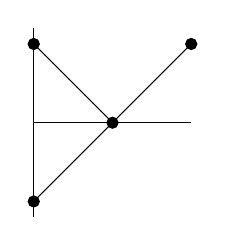
\begin{tikzpicture}
        \draw (0,1) -- (1,0) -- (2,1);
        \draw (0,-1) -- (1,0);
        \draw (0,-1.2) -- (0,1.2);
        \draw (0,0) -- (2,0);
        \foreach \x in {(0,1),(0,-1),(1,0),(2,1)}
            \filldraw \x circle (2pt);
    \end{tikzpicture}
\end{center}

Let $(S_n)$ be a symmetric simple random walk on $\Z$.
\begin{theorem}
    Let $n \in \N$. Then $P(S_1 \neq 0, \dots, S_{2n} \neq 0) = P(S_{2n} = 0)$.
\end{theorem}
\begin{proof}
    By symmetry, $P(S_1 > 0, \dots, S_{2n} > 0) = P(S_1 < 0, \dots, S_{2n} < 0)$. Now $(S_n)$ cannot change sign without passing through $0$. Hence $P(S_1 > 0, \dots, S_{2n} > 0) + P(S_1 < 0, \dots, S_{2n} < 0) = P(S_1 \neq 0, \dots, S_{2n} \neq 0)$. Now $P(S_1 > 0, \dots, S_{2n} > 0) = \sum_{r = 1}^n P(S_1 > 0, \dots, S_{2n-1} > 0, S_{2n} = 2r)$. The number of paths from $(0,0)$ to $(2n, 2r)$ that are never $0$ at times $\geq 1$ is equal to the number of paths from $(1,1)$ to $(2n,2_r)$ that are never 0, and this is equal to $K_r - J_r$ where $k_r$ is the number of paths from $(1,1)$ to $(2n, 2r)$ and $J_r$ is the number of such paths that are 0 at some time. By the reflection principle, $J_r$ is equal to the number of paths from $(1,-1)$ to $(2n,2r)$. Thus $J_r$ is the number of paths from $(1,1)$ to $(2n, 2(r+1))$. In other words, $J_r = K_{r+1}$. Thus the number of paths from $(0,0)$ to $(2n, 2r)$ that are never $0$ at times $\geq 1$ is equal to $K_r - K_{r+1}$. Hence $P(S_1 > 0, \dots, S_{2n-1} > 0, S_{2n} = 2r) = (K_r - K_{r+1})/2^{2n}$. So
    \[
        P(S_1 > 0, \dots, S_{2n} > 0) = \sum_{r=1}^n \frac{K_r - K_{r+1}}{2^{2n}} = \frac{K_1 - K_{n+1}}{2^{2n}}.
    \]
    But $K_{n+1} = 0$, because $2(n+1) - 1 > 2n - 1$. Also $K_1$ is the number of paths from $(1,1)$ to $(2n,2)$ and this is equal to the number of paths from $(0,0)$ to $(2n-1, 1)$, which is $\binom{2n-1}{n}$, since such paths have $n$ steps of $+1$ and $n-1$ steps of $-1$. Thus
    \[
        P(S_1 > 0, \dots, S_{2n > 0}) = \frac{1}{2}\binom{2n-1}{n}\frac{1}{2^{2n-1}} = \frac{1}{2}P(S_{2n-1} = 1).
    \]
    To finish, observe that $P(S_{2n} = 0) = P(S_{2n-1} = -1, X_{2n} = 1) + P(S_{2n-1} = 1, X_{2n} = -1) = (1/2)P(S_{2n - 1} = -1) + (1/2)P(S_{2n - 1} = 1)$.
\end{proof}

\begin{corollary}
    Let $R$ be the first time $(S_n)$ returns to 0. In other words, let $R = \inf\{m \geq 1 : S_m = 0\}$. Then $P(R > 2n) \sim 1/\sqrt{\pi n}$ as $n \to \infty$.
\end{corollary}
\begin{proof}
    \begin{align*}
        P(R = 2n) &= P(S_1 \neq 0, \dots, S_{2n} \neq 0) = P(S_{2n} = 0) \\
        \intertext{by the theorem}
        &= \binom{2n}{n}\frac{1}{2^{2n}} = \frac{(2n)!}{(n!)^2}\frac{1}{2^{2n}} \sim \frac{\sqrt{2\pi 2n}(2n)^{2n} e^{-2n}}{(\sqrt{2\pi n} n^n e^{-n})^2}\frac{1}{2^{2n}} \\
        \intertext{as $n \to \infty$, by Stirling's formula}
        &= \frac{\sqrt{2\pi 2n}}{2\pi n} \frac{n^{2n}}{n^{2n}} \frac{2^{2n}}{2^{2n}} \frac{e^{-2n}}{e^{-2n}} = \frac{1}{\sqrt{\pi n}}.
    \end{align*}
\end{proof}

\begin{remark}
In particular, $P(R > 2n) \to 0$ as $n \to \infty$, so $P(R = \infty) = 0$. But in fact,
\[
    E(|\{n : S_{2n} = 0\}|) = E\left(\sum_{n=0}^\infty 1_{\{0\}}(S_{2n}\right) = \sum_{n=0}^\infty E(1_{\{0\}}(S_{2n})) = \sum_{n=1}^\infty P(S_{2n} = 0) = \infty
\]
since $P(S_{2n} = 0) \sim 1/\sqrt{\pi n}$ as $n \to \infty$.
\end{remark}

\begin{notation}
Let $L_{2n} = \max\{m \leq 2n : S_m = 0\}$ (this set is nonempty, because 0 belongs to it). $L_{2n}$ is the last time the players are all square, if they play for $2n$ tosses.
\end{notation}

\begin{proposition}
    Let $k \in \{0, \dots, n\}$. Then $P(L_{2n} = 2k) = P(S_{2k} = 0) = P(S_{2n - 2k} = 0)$.
\end{proposition}
\begin{proof}
    \begin{align*}
        P(L_{2n} = 2k) &= P(S_{2k} = 0, S_{k+1} \neq 0, \dots, S_{2n} \neq 0) = P(S_{2k} = 0, \underbrace{S_{2k+1} - S_{2k} \neq 0, \dots, S_{2n} - S_{2k} \neq 0}_{\text{independent of } S_{2k}}) \\
        &= P(S_{2k = 0})P(S_{2k+1} - S_{2k} \neq 0, \dots, S_{2n} - S_{2k} \neq 0) \\
        &= P(S_{2k = 0})P(S_1 \neq 0, \dots, S_{2n-2k} \neq 0) = P(S_{2k} = 0)P(S_{2n-2k} = 0)
    \end{align*}
    by the theorem.
\end{proof}

\begin{remark}
It follows that the distribution of $L_{2n}$ in $\{0, 2, \dots, 2n\}$ is symmetric about $n$. Thus if two people were to bet $\$1$ on a coin flip each day for a year, then with probability at least $1/2$ one of them will be ahead from early July to the end of the year, which might cause the other to complain about his bad luck. (January - June is 181 or 182 days, July - December is 184 days).
\end{remark}

\begin{theorem}[The Arcsine Law for $L_{2n}$]
 Let $0 < b < 1$. Then as $n \to \infty$,
 \[
    P\left(a < \frac{L_{2n}}{2n} < b\right) \to \int_a^b \frac{1}{\pi\sqrt{x(1-x)}} \,dx = \frac{2}{\pi}(\operatorname{arcsin}\sqrt{b} - \operatorname{arcsin}\sqrt{a}).
 \]    
\end{theorem}
\begin{proof}
    Let $K_n = \P; : a \leq (2k)/(2n) \leq b\}$. As $n \to \infty$,
    \begin{align*}
        P(L_{2n} \leq 2k) &= P(S_{2k} = 0)P(S_{2n-2k} = 0) \sim \frac{1}{\sqrt{\pi}k}\frac{1}{\sqrt{\pi(n-k)}} \\
        \intertext{(This holds uniformly for $k \in K_n$, because for each $k$, we have $2k \geq 2na$ and $2n - 2k \geq 2n(1-b)$.) Let $x_{n,k} = k/n$.}
        &= \frac{1/n}{\pi\sqrt{k/n}(1-k/n)} = \frac{1}{\pi\sqrt{x_{n,k}(1-x_{n,k})}}(x_{n,k} - x_{n,k-1}).
    \end{align*}
    Therefore
    \begin{align*}
        P\left(a \leq \frac{L_{2n}}{2n} \leq b\right) &\sim \sum_{k \in K_n} \frac{1}{\pi\sqrt{x_{n,k}(1-x_{n,k})}} (x_{n,k} - x_{n,k-1}) \to \int_a^b \frac{1}{\pi\sqrt{x(1-x)}} \,dx \\
        \intertext{Let $y = \sqrt{x}$, so $y^2 = x$, $2y\,dy = dx$; $a \xrightarrow{x} b$, $\sqrt{a} \xrightarrow{y} \sqrt{b}$.}
        &= \int_{\sqrt{a}}^{\sqrt{b}} \frac{1}{\pi}\frac{1}{y} \frac{1}{\sqrt{1-y^2}}2y\,dy = \frac{2}{\pi} \int_{\sqrt{a}}^{\sqrt{b}} \frac{1}{1-y^2} \,dy = \frac{2}{\pi}(\operatorname{arcsin}\sqrt{b} - \operatorname{arcsin}\sqrt{a}).
    \end{align*}
\end{proof}

\section{4/21/21}
\subsection*{On Midterm 2.}

\textbf{Problem 1.}
\begin{enumerate}[(a)]
    \item \begin{align*}
        P(H = k) &= \sum_{n = k}^6 P(H = k, D = n) = \sum_{n = k}^6 P(H = k \mid D = n)P(D = n) \\
        &= \sum_{n = k}^6 \binom{n}{k}\left(\frac{1}{2}\right)^k \left(\frac{1}{2}\right)^{n-k} \frac{1}{6} = \sum_{n = k}^6 \binom{n}{k}\frac{1}{2^n}\frac{1}{6}
    \end{align*}
    \item If $3$ heads are obtained, what is the probability that the die showed $n$?
    \begin{align*}
        P(D = n \mid H = 3) &= \frac{P(D = n, H = 3)}{P(H = 3)} \\
        &= \frac{P(H = 3 \mid D = n)P(D = n)}{P(H = 3)}.
    \end{align*}
    $P(H = 3) = \sum_{n = 3}^6 \binom{n}{3}2^{-n}/6 = \dots = 1/6 = P(D = n)$. Hence $P(D = n \mid H = 3) = P(H = 3 \mid D = n) = \binom{n}{3}2^{-n}$.
\end{enumerate}

\begin{remark}[A False Generalization of the Monotone Convergence Theorem]
Let $(X, \mathscr{A}, \mu)$ be a measure space. Let $f$ be a nonnegative measurable function on $X$. Let $(f_n)$ be a sequence of nonnegative measurable functions on $X$. Suppose that for all $x \in X$, $f_n(x) \to f(x)$ as $n \to \infty$ there is an $n_0 \in \N$ such that for each $n \geq n_0$, $f_n(x) \leq f_{n+1}(x)$. Then $\int f_n \,d\mu \to \int f \,d\mu$.
\begin{center}
    \Huge{NO!!!}
\end{center}
\end{remark}
\begin{example}
Let $f_n = 1_{[n, \infty)}$. Then $f_n \to 0$ pointwise on $\R$. Let $x \in \R$. Let $n_0 = \lfloor x \rfloor + 1$. Then for all $n \geq n_0$, $f_n(x) = f_{n+1}(x)$ (because both are $0$).
\end{example}

\textbf{Problem 2.} Let $X$ be a random variable and let $\varphi(u) = E(e^{iuX})$.
\begin{align*}
    \frac{2 - \varphi(u) - \varphi(-u)}{u^2} &= E\left(\frac{2 - e^{iuX} - e^{-iuX}}{u^2}\right) = E\left(\frac{2 - 2\cos(uX)}{u^2}\right) \\
    &= E\left(\frac{4\sin^2(uX/2)}{u^2}\right) = E\left[\left(\frac{\sin(uX/2)}{u/2}\right)^2\right].
\end{align*}
If $v \neq 0$, then $\sin(uv)/u = v\sin(uv)/(uv) \to v \cdot 1 = v$ as $u \to 0$. If $f = 0$, then $\sin(uv)/u - 0 = v \to v$ as $u \to 0$. Thus
\[
    \left(\frac{\sin(uX/2)}{u/2}\right)^2 \to X^2 \text{ as } u \to 0.
\]
Now $|\sin\theta| \leq |\theta|$ for $\theta$ real. Thus
\[
    0 = \left(\frac{\sin(uX/2)}{u/2}\right)^2 \leq \left(\frac{uX/2}{u/2}\right) = X^2.
\]
Hence by a corollary of Fatou's lemma,
\[
    E\left[\left(\frac{\sin(uX/2)}{u/2}\right)^2\right] \to E(X^2).
\]
\begin{remark}
To be completely correct, one should replace $u$ with a sequence $u_n \to 0$, but the above analysis is necessary; it is not enough, for example, to consider $u$ along $1/n$.
\end{remark}
\begin{example}
Let
\[
    f(x) = \begin{cases}
        \frac{1}{n} &\text{if } x = \frac{1}{n} \text{ where } n \in \N \\
        1 &\text{otherwise}.
    \end{cases}
\]
Then $\lim_{n \to \infty} f(1/n) = 0$ but $\lim_{x \to 0} f(x)$ does not exist.
\end{example}
\begin{example}
Let $f = 1$ on $\R$. Let $f_A = 1_A$ for each finite $A \subseteq \R$. Then $f_A \to f$ pointwise as $A \uparrow \R$. But for all finite $A \subseteq \R$, $\int_\R f_A(x) \,dx = 0$ so $\int f_A \not\to \int f$ as $A \uparrow \R$.
\end{example}

\section*{4/23/21}
\begin{remark}[On Extra Problem 47]
Let $S_n' = (S_n)^\circ$. Then $S_n' = S_n - (p-q)n$, so $S_{T_b}' = S_{T_b} - (p-q)T_b = b - (p-q)T_b$. Also, by Wald's second equation, $E[(S_{T_b}')^2] = E[(X_1^\circ)^2]E(T_b)$ and $E[(X_1^\circ)^2] = E(X_1^2) - E(X_1)^2 = 1 - (p-q)^2$.

Note that $0 = (S_{T_b})^\circ \neq (S^\circ)_{T_b}= S_{T_b}'$.
\end{remark}

% This part does not translate well to typed notes
% Falkner is talking about how to handwrite script letters
\subsection*{On Handwriting Script Letters, Typeset Edition.}
Don't write $\mathscr{Q}$, $\mathscr{X}$, or $\mathscr{Z}$.

$\mathscr{A}, \mathscr{B}, \mathscr{C}, \mathscr{D}, \mathscr{E}, \mathscr{F}, \mathscr{G}, \mathscr{H}, \mathscr{I}, \mathscr{J}, \mathscr{K}, \mathscr{L}, \mathscr{M}, \mathscr{N}, \mathscr{O}, \mathscr{P}, ?, \mathscr{R}, \mathscr{S}, \mathscr{T}, \mathscr{U}, \mathscr{V}, \mathscr{W}, \mathscr{X}, \mathscr{Y}, ??$

\subsection*{Brownian Motion in $\R^d$.}
Let $\Omega = C([0,\infty), \R^d)$ (the set of continuous paths in $\R^d$), $B_t(\omega) = \omega(t)$ (the location of a path at $t$), $\F^\circ = \sigma(B_t : 0 \leq t < \infty)$. For each $x \in \R^d$, let $P^x$ be the probability distribution of paths starting at $x$, $P^x(B_0 = x) = 1$. For $t > 0$,
\[
    P^x(B_t \in dy) = P_t(x, dy) = p_t(x,y) = \left(\frac{1}{2\pi t}\right)^{d/2} e^{-|x-y|^2/(2t)} \,dy.
\]
\begin{remark}
For all $\varepsilon > 0$, $t^{-1} \sup_x P_t(x : \{y : \operatorname{dist}(x,y) \geq\varepsilon\}) \to 0$ as $t \downarrow 0$. This is why we can construct that $P^x$'s on $C([0, \infty), \R^d)$. Compare with the Cauchy process (for $d = 1$)
\[
    Q_t(x,dy) = \frac{t/\pi}{(x-y)^2 + t^2}\,dy.
\]
\end{remark}

\subsection*{Joint distributions for $(B_t)$.}
For $0 < t_1 < t_2 < \dots < t_n < \infty$, for $A_1, A_2, \dots, A_n \in \Borel(\R^d)$,
\[
    P^x(B_{T_1} \in A_1, B_{T_2} \in A_2, \dots, B_{T_n} \in A_n) = \int_{A_1} P^x(B_{t_1} \in dy)P^y(B_{t_2 - t_1} \in A_2, \dots, B_{T_n - t_{n-1}} \in A_n)
\]
(this is the \emph{Markov property}).
\[
    P^x(B_{t_1} \in dy_1, B_{t_2} \in y_2, \dots, B_{T_n} \in dy_n) = P_{t_1}(x, dy_1)P_{t_2 - t_1}(y_1, dy_2) \cdots P_{t_n - t_{n-1}}(y_{n-1}, dy_n).
\]
$(B_t)$ has stationary independent increments:
\[
    E^x[f_1(B_{t_1} - B_0)f_2(B_{t_2} - B_{t_1}) \cdots f_n(B_{t_n} - B_{t_{n-1}})] = E^0[f_1(B_{t_1})]E^0[f_2(B_{t_2})] \cdots E^0[f_n(B_{t_n - t_{n-1}})].
\]

\subsection*{Stochastic Integrals.} ($d = 1$ for now)
\[
    \int_0^1 C_t \,dB_t
\]
$C_t$ should be \emph{non-anticipating}: $C_t(\omega) = f(t, (B_s(\omega))_{0 \leq s \leq t})$. If not, bad things can happen Say $C_t^n(\omega) = \sum_{k=0}^{2^n - 1} Y_k^n(\omega)1_{(t_k^n < t \leq t_{k+1}^n)}$, where $t_k^n = k/2^n$. Then $\int_0^1 C_t^n \,dB_t$ should be
\[
    I_n = \sum_{k=0}^{2^n-1} Y_k^n \cdot \Delta_k^n
\]
where $\Delta_k^n = B_{t_{k+1}^n} - B_{t^n_k}$. Consider $Y_k^n = \sgn(\Delta_k^n)/n$. (Then $(C_t^n)$ is anticipating.) Note that $E^0(|B_t|^p) = \int_\R (|x|^p/\sqrt{2\pi t})e^{-x^2/(2t)} \,dx = \gamma_pt^{p/2}$ (for some $\gamma_p \in (0, \infty)$). Then
\[
    E(|\Delta^n_k|) = \gamma_1 2^{-n/2}
\]
\[
    \var(|\Delta^n_k|) = E(|\Delta^n_k|^2) - E(|\Delta^n_k|)^2 = 2^{-n} - (\gamma_1 2^{-n/2})^2 = c_22^{-n}.
\]
So,
\[
    E(I_n) = \frac{2^n}{n}\gamma_1 2^{-n/2} = \gamma_1\frac{2^{n/2}}{n}.
\]
\[
    \var(I_n) = \frac{1}{n^2}\sum_{k=0}^{2^n-1} \var(|\Delta^n_k|) = \frac{c_2}{n^2}.
\]
Thus
\[
    E\left[\sum_{n=1}^\infty (I_n - E(I_n))^2\right] = \sum_{n=1}^\infty \var(I_n) = \sum_{n=1}^\infty \frac{c_2}{n^2} < \infty
\]
so $\sum_{n=1}^\infty (I_n - E(I_n))^2 < \infty$ almost surely so $I_n - E(I_n) \to 0$ almost surely so $I_n \to \infty$ almost surely. Thus, even though $|C^n_t| \leq 1/n \to 0$, so $|C^n_t| \to 0$ uniformly on $\Omega \times [0,1]$, we have $\int C^n_t \,dB_t \to \infty$ almost surely.

Actually, $I_n = n^{-1}\sum_{k=0}^{2n-1} |\Delta^n_k|$. Thus $\sum_{k=0}^{2^n-1} |\Delta^n_k| \to \infty$ almost surely. Thus almost every Brownian path has infinite arc length.

A similar calculation shows that $\sum_{k=0}^{2^n-1} (B_{t^n_{k-1}} - B_{t^n_k})^2 \to 1$ almost surely. This is related to Taylor's formula: $\int_0^t f'(B_s)\,dB_0 = f(B_t) - f(B_0) + \int_0^t f''(B_s)/2 \,ds$.

\end{document}